\documentclass{cumcmthesis}
\usepackage{amsmath,amssymb,amsfonts,bm}
\usepackage{booktabs,array,longtable}
\usepackage{graphicx}
\usepackage{xcolor}
\usepackage{caption}
\usepackage{subcaption}
\usepackage{float}
\usepackage{enumitem}
\usepackage{hyperref}
\usepackage{listings}

\hypersetup{
    colorlinks=true,
    linkcolor=black,
    citecolor=black,
    urlcolor=black,
    pdftitle={基于离散刚体运动学的板凳龙路径规划与干涉分析}
}

% ============================================================
% 核心排版参数设置 
% ============================================================
\setlength{\parindent}{2em}
\setlength{\parskip}{0.4em} 
\linespread{1.35} 

% ============================================================
% 代码块高级格式设置 
% ============================================================
\lstset{
    language=Python,
    basicstyle=\ttfamily\small,
    breaklines=true,
    columns=fullflexible,
    frame=single,
    numbers=left,
    numberstyle=\tiny\color{gray},
    keywordstyle=\color{blue}\bfseries,
    commentstyle=\color{green!50!black},
    stringstyle=\color{purple},
    showstringspaces=false,
    extendedchars=false
}

% ============================================================
% 自定义数学命令
% ============================================================
\newcommand{\norm}[1]{\left\lVert #1 \right\rVert}

% ============================================================
% 图片占位命令 (为组长后续插图预留)
% ============================================================
\newcommand{\figureplaceholder}[3]{%
\begin{figure}[H]
    \centering
    \fbox{%
      \begin{minipage}[c][0.2\textheight][c]{0.8\textwidth}
        \centering
        \zihao{-4}
        \textcolor{gray}{[图表位置：#1]}\\[4pt]
        \texttt{（请在此处插入相关图片，建议使用 PDF 或高清 PNG 格式）}
      \end{minipage}}
    \caption{#2}
    \label{#3}
\end{figure}
}

% ============================================================
% 标题及队伍信息
% ============================================================
\title{基于离散刚体运动学的板凳龙路径规划与干涉分析}
\tihao{A}            
\baominghao{66666666}    
\schoolname{上海电机学院}
\membera{黄张}
\memberb{李雨树}
\memberc{张天毅}
\supervisor{武文佳}
\yearinput{2026}     
\monthinput{08}      
\dayinput{27}        

\begin{document}
\maketitle

% ============================================================
% 摘要
% ============================================================
\begin{abstract}
“板凳龙”由 $223$ 节刚性板凳经把手铰接而成，其盘入盘出是受螺线轨迹与刚性连接双重约束的离散多体运动学问题。本文以“几何逆推—干涉检测—参数优化—安全认证”为主线，建立覆盖五问的统一模型体系。

针对问题一，建立\textbf{基于弧长—极角积分与几何逆推的运动学模型}：由龙头匀速条件反解其极角，以相邻弦长约束逐节 Brent 逆推 224 个把手坐标，再以刚体链速度分解递推验证中心差分结果。算得全链各把手速度\textbf{均近似 $1\,\mathrm{m/s}$}，与刚性链无滑移的物理预期一致。

针对问题二，建立\textbf{SAT 与顶点包容相结合的混合干涉判据及连续碰撞检测（CCD）模型}：以旋转矩形建模板凳实体，AABB 宽相预筛控制复杂度，带符号间隙函数配合黄金分割消除固定步长的“隧道效应”，二分逼近临界时刻。算得盘入终止时刻 $\boldsymbol{t^{*}=412.47\,\text{s}}$，首次干涉发生于\textbf{龙头与第 9 节板凳之间}。

针对问题三，建立\textbf{以螺距为唯一决策变量的一维黑盒约束优化模型}：边界条件 $r(\theta_{\mathrm{end}})=4.5\,\mathrm{m}$ 锁定盘入终点，以“全程无非相邻板凳相交（SAT）”为非光滑碰撞约束，论证可行性关于螺距单调后二分求解。算得最小螺距 $\boldsymbol{p^{*}\approx 0.4503\,\mathrm{m}}$（区间宽 $10^{-4}\,\mathrm{m}$），临界干涉始终发生于龙头与相邻圈第 18~20 节之间。

针对问题四，建立\textbf{基于两弧相切解析几何与复合轨迹逆推的调头模型}：由中心对称性与外切条件解析确定 S 形曲线，$\boldsymbol{L_0=13.6212\,\mathrm{m}}$ 恰内切调头空间，逆推法推广至复合轨迹完成 $-100\sim100\,\text{s}$ 全链递推；证明\textbf{切点固定的两弧族长度不变性定理}——仅调半径比例不能变短；进而引入弧–线–弧结构最优化得 $\boldsymbol{L^{*}=10.0642\,\mathrm{m}}$（\textbf{缩短 26.11\%}），全程无碰撞。

针对问题五，建立\textbf{基于齐次性约化的速度比场全局优化模型}：运动学对龙头速度线性齐次，把“任意时刻、任意把手速度 $\le 2\,\text{m/s}$”的无穷族约束化为\textbf{一元全局最大化} $v^{*}=2/R_{\max}$；以\textbf{接缝事件分解把搜索轴切成有限个光滑段}，段内驻点求根精确最大化，辅以\textbf{Lipschitz 剪枝证书与事件子段穷举}完成全局最优性认证（宽度 $<10^{-9}$），并以弦切角公式与同弧段恒速引理解析峰值机理。算得 $R_{\max}=1.604793379$，\textbf{龙头最大行进速度 $v^{*}=1.246266\,\text{m/s}$}，$t^{*}_{5}=11.62\,\text{s}$ 时第 4--8 把手并列达 $2\,\text{m/s}$，峰值分解为\textbf{跨 $F$ 缝因子 $1.5542\times$ 跨 $T$ 缝因子 $1.0325$}；对问题四弧–线–弧缩短曲线复核发现临界半径处速度比无界、$v^{*}$ 骤降 $93\%$——\textbf{“盘得紧”与“跑得快”不可兼得}。

\keywords{离散运动学 \quad 几何逆推 \quad 分离轴定理(SAT) \quad 连续碰撞检测(CCD) \quad 二分搜索 \quad 不变性定理 \quad 齐次性约化 \quad 速度传递比 \quad 全局优化与认证}
\end{abstract}

% \tableofcontents % 电子版正式提交时通常不需要目录

\section{问题背景}

“板凳龙”，又称“盘龙”，是浙闽地区的传统地方民俗文化活动：少则几十条、多则上百条板凳首尾相连，龙头在前领头、龙身龙尾相随盘旋，整体呈圆盘状。在舞龙队能自如盘入盘出的前提下，盘龙所需面积越小、行进速度越快，观赏性越好。从运动学角度看，$223$ 节板凳经把手铰接构成受螺线轨迹约束与刚性连接约束的\textbf{离散多体系统}（广义 N 拖车铰接链）：随盘入半径减小、曲率增大，各节点速度差异加剧，不同圈层的非相邻板凳极易发生空间干涉。因此，精确计算各节点运动状态并评估避碰安全边界、进而在安全约束下优化路径与速度，是理解并优化这一传统表演的核心问题。

\section{问题重述}

\textbf{问题一}\quad 舞龙队沿螺距 $55\,\text{cm}$ 的等距螺线顺时针盘入，各把手中心均位于螺线上，龙头前把手恒速 $1\,\text{m/s}$，初始位于第 $16$ 圈 $A$ 点。求 $0\sim300\,\text{s}$ 每秒整条舞龙队（$224$ 个节点）的位置与速度，结果保留 6 位小数写入文件，并在论文中给出 $t=0,60,\dots,300\,\text{s}$ 时龙头前把手、第 $1/51/101/151/201$ 节龙身前把手及龙尾后把手的位置与速度。

\textbf{问题二}\quad 沿问题一螺线盘入，确定盘入的\textbf{终止时刻}——板凳间即将发生碰撞、不能再继续盘入的时刻，给出此时全龙位置与速度并写入文件，同时在论文中给出各关键把手的位置与速度。

\textbf{问题三}\quad 设调头空间为以螺线中心为圆心、直径 $9\,\text{m}$ 的圆形区域，确定\textbf{最小螺距}，使龙头前把手能沿相应螺线无碰撞地盘入调头空间边界。

\textbf{问题四}\quad 螺距取 $1.7\,\text{m}$，盘出螺线与盘入螺线中心对称，舞龙队在调头空间内经两段相切圆弧构成的 S 形曲线调头（$R_1=2R_2$，与两螺线均相切）。以调头开始为 $0$ 时刻给出 $-100\sim100\,\text{s}$ 每秒全龙位置与速度（写入文件并给出 5 个关键时刻的表格）；进一步分析：能否调整圆弧、仍保持各部分相切使调头曲线变短？

\textbf{问题五}\quad 沿问题四路径行进，龙头速度恒定但大小待定，确定龙头的\textbf{最大行进速度} $v^{*}$，使全程各把手速度均不超过 $2\,\text{m/s}$。

\section{问题分析}

\textbf{问题一的分析}\quad 本问属\textbf{刚体链在给定曲线上的逆运动学}：由弧长积分方程反解龙头极角，再以“相邻把手间距恒定”与“各把手均在螺线上”两大约束建立逐节非线性距离方程，取极角最接近前驱的交点逐节 Brent 逆推；速度以细步长中心差分求得，并用刚体铰接链速度分解递推独立验证。

\textbf{问题二的分析}\quad 本问是\textbf{动态旋转矩形的相交测试}与首次干涉时刻搜索，要点有三：常规边交点检测漏检“矩形完全包含”退化情形，须引入分离轴定理（SAT）与顶点包容检验；$223$ 节板凳两两检测计算量大，以外接包围盒（AABB）作宽相预筛；固定步长会产生“隧道效应”漏检，须定义带符号间隙函数在连续时间域上极值化以捕捉接触瞬间。

\textbf{问题三的分析}\quad 本问是“盘入可达性”约束下的\textbf{一维黑盒约束优化}：螺距 $p$ 给定后螺线族与盘入终点（$\theta_{\mathrm{end}}=9\pi/p$）随之确定，决策变量只有 $p$，目标线性而难点全在非光滑的碰撞约束——须逐构型调用问题二的干涉判据，无解析梯度。螺距增大时相邻螺圈径向间隙单调增大，可行性关于 $p$ 单调，故采用二分搜索收缩区间至 $10^{-4}\,\mathrm{m}$；入口处螺线与调头圆近乎曲率连续，为问题四的调头路径设计提供平滑衔接。

\textbf{问题四的分析}\quad 第一问仍是逆运动学，但龙头轨迹变为“盘入螺线—圆弧—圆弧—盘出螺线”复合曲线：须先由中心对称性与外切条件\textbf{解析解出} S 形几何，再把逆推法推广为复合轨迹上的弦长递推。“能否变短”须区分两种自由度：切点固定后两弧外切条件把 $R_1+R_2$ 与扫角均锁定为几何常量——两弧族内长度是\textbf{不变量}，仅调半径比例不能变短；打破结构约束、允许弧间引入公切线段（弧–线–弧）方可缩短，缩短后的曲线须再经全龙碰撞检测验证可行。

\textbf{问题五的分析}\quad 约束是“时间 $\times$ 把手”的二维无穷族。注意到构型仅由龙头弧长位置 $u_1$ 决定且运动学对速度\textbf{线性齐次}：$v_i(t)=v\,\rho_i(u_1)$，$\rho_i$ 为纯几何的速度传递比——约束化为 $v\le 2/R_{\max}$ 的\textbf{一元全局最大化}。难点在速度比场于曲率切换接缝附近呈尖峰（弦切角机制使放大集中于小半径弧段一侧），而网格采样会因漏峰系统性高估容许速度且无收敛证书，故建立“接缝事件分解—驻点求根—双层认证”模型，并给出峰值机理分解与“调头曲线长度—行进速度”的权衡分析。

\section{模型假设与符号说明}

\subsection{模型假设}
\begin{enumerate}[label=(\arabic*), itemsep=0.3em]
    \item 忽略相邻板凳在把手连接处的物理间隙与机械形变（孔径 $5.5\,\text{cm}$ 不影响链条构型），视前后孔距为绝对刚性约束。
    \item 系统运动处于理想水平二维平面内，忽略板凳在三维方向上的俯仰与侧倾。
    \item 龙头行进速度保持严格恒定，不考虑实际中因人力驱动产生的瞬时速度波动；问题五中龙头速度大小待定，但同样保持恒定。
    \item 各把手中心精确位于给定轨迹曲线（螺线或复合轨迹）上；板宽 $30\,\text{cm}$ 仅在碰撞检测中作为实体尺寸考虑，不影响运动学轨迹。
    \item 除题目要求检测的干涉情形外，行进全程板凳之间保持无碰撞；问题四、问题五所采用的路径与速度均已通过全龙碰撞检测验证可行。
\end{enumerate}

\subsection{符号说明}
\renewcommand{\arraystretch}{1.2}
\begin{table}[H]
\centering
\caption{主要变量与参数符号说明}
\begin{tabular}{clc}
\toprule
符号 & 物理含义 & 单位/量纲 \\
\midrule
$p$ & 等距螺线的螺距（本题取 $p=55$） & cm \\
$b$ & 极坐标螺线方程的极径系数 ($b = p / 2\pi$) & m/rad \\
$v_{0}$ & 龙头前把手的恒定行进线速度（$1\,\text{m/s}$） & m/s \\
$L_i$ & 第 $i$ 节板凳前后把手孔之间的有效间距 & m \\
$(x_i(t), y_i(t))$ & 任意 $t$ 时刻，第 $i$ 个把手节点的直角坐标 & m \\
$\theta_i(t)$ & 任意 $t$ 时刻，第 $i$ 个把手节点的极角 & rad \\
$S(t)$ & $t$ 时刻龙头沿等距螺线走过的总弧长 & m \\
$t^*$ & 系统盘入至发生首次实体干涉的终止时刻 & s \\
$R$ & 调头空间半径（直径 $9\,\text{m}$） & m \\
$\theta_{\mathrm{end}}$ & 龙头前把手到达调头空间边界时的极角 & rad \\
$p^{*}$ & 龙头可无碰撞盘入调头空间边界的最小螺距 & m \\
\midrule
$E,\,F$ & 调头路径与盘入、盘出螺线的切点 & m \\
$R_1,\,R_2$ & S 形曲线两段圆弧的半径（$R_1=2R_2$） & m \\
$\gamma$ & S 形曲线单段圆弧的扫角（两弧相等） & rad \\
$L_0$ & S 形调头曲线的总长 & m \\
$u$ & 复合轨迹沿行进方向的弧长参数（$u=0$ 在入口切点） & m \\
$\ell$ & 弧–线–弧结构中的公切线段长 & m \\
$L^{*}$ & 相切约束下最短的调头曲线长度 & m \\
\midrule
$v^{*}$ & 各把手速度 $\le 2\,\text{m/s}$ 约束下龙头的最大行进速度 & m/s \\
$\rho_i(u_1)$ & 龙头单位速度下第 $i$ 把手的速度传递比（纯几何量） & 无量纲 \\
$R_{\max}$ & 速度传递比场的全局最大值（$v^{*}=2/R_{\max}$） & 无量纲 \\
$u_1$ & 龙头前把手沿复合轨迹的弧长位置（$u_1=0$ 在切点 $E$） & m \\
$\alpha_j,\,\beta_j$ & 第 $j$ 根弦在前、后把手处的弦切角 & rad \\
$t^{*}_{5}$ & 以 $v^{*}$ 行进时速度比达到 $R_{\max}$ 的临界时刻 & s \\
\bottomrule
\end{tabular}
\end{table}
\renewcommand{\arraystretch}{1.0}

%% ========================================================
%% 第五、六章：问题一/问题二模型的建立与求解
%% ========================================================
\section{问题一模型的建立和求解}

\subsection{模型建立}

\subsubsection{螺线轨迹与龙头运动方程}
等距螺线（阿基米德螺线）的极坐标方程为
\begin{equation}
r(\theta) = b\theta, \qquad b = \frac{p}{2\pi} = \frac{0.55}{2\pi}\,\text{m/rad},
\end{equation}
其中螺距 $p=55\,\text{cm}$ 保证相邻两圈径向间距恰为一个螺距。该类等距螺线是路径规划中过渡曲线的基本形态之一，其曲率沿弧长连续变化，避免了圆弧—直线衔接处的曲率突变~\cite{lekkas}。初始时刻 $t=0$ 时龙头位于第 16 圈，即极角 $\theta_0 = 32\pi$、极径 $r_0=16p=8.8\,\text{m}$。龙头前把手以恒定线速度 $v_0 = 1\,\text{m/s}$ 沿螺线切向顺时针盘入，弧长微元满足
\begin{equation}
\mathrm{d}s=\sqrt{r^2(\alpha)+\left[r'(\alpha)\right]^2}\,\mathrm{d}\alpha
= b\sqrt{\alpha^2+1}\,\mathrm{d}\alpha .
\end{equation}
由 $S(t)=v_0 t$ 得弧长—极角积分方程
\begin{equation}
S(t) = \int_{\theta_1(t)}^{\theta_0} b\sqrt{\alpha^2+1}\,\mathrm{d}\alpha
= \frac{b}{2} \left[ \alpha \sqrt{\alpha^2+1} + \ln\!\left(\alpha + \sqrt{\alpha^2+1}\right) \right] \Bigg|_{\theta_1(t)}^{\theta_0} = t .
\end{equation}
该式左端关于 $\theta_1(t)$ 严格单调，故对任意 $t\in[0,300]$ 存在唯一根，可由二分法数值反解出龙头极角，进而得到龙头直角坐标 $(x_1,y_1)=\bigl(b\theta_1\cos\theta_1,\ b\theta_1\sin\theta_1\bigr)$。整条龙沿螺线盘入的整体几何关系如图~\ref{fig:spiral_overview} 所示，各把手中心均落在螺线上，其位置完全由极角确定，相邻把手的极角差 $\Delta\theta$ 由板长与所在圈半径共同决定。

\begin{figure}[H]
\centering
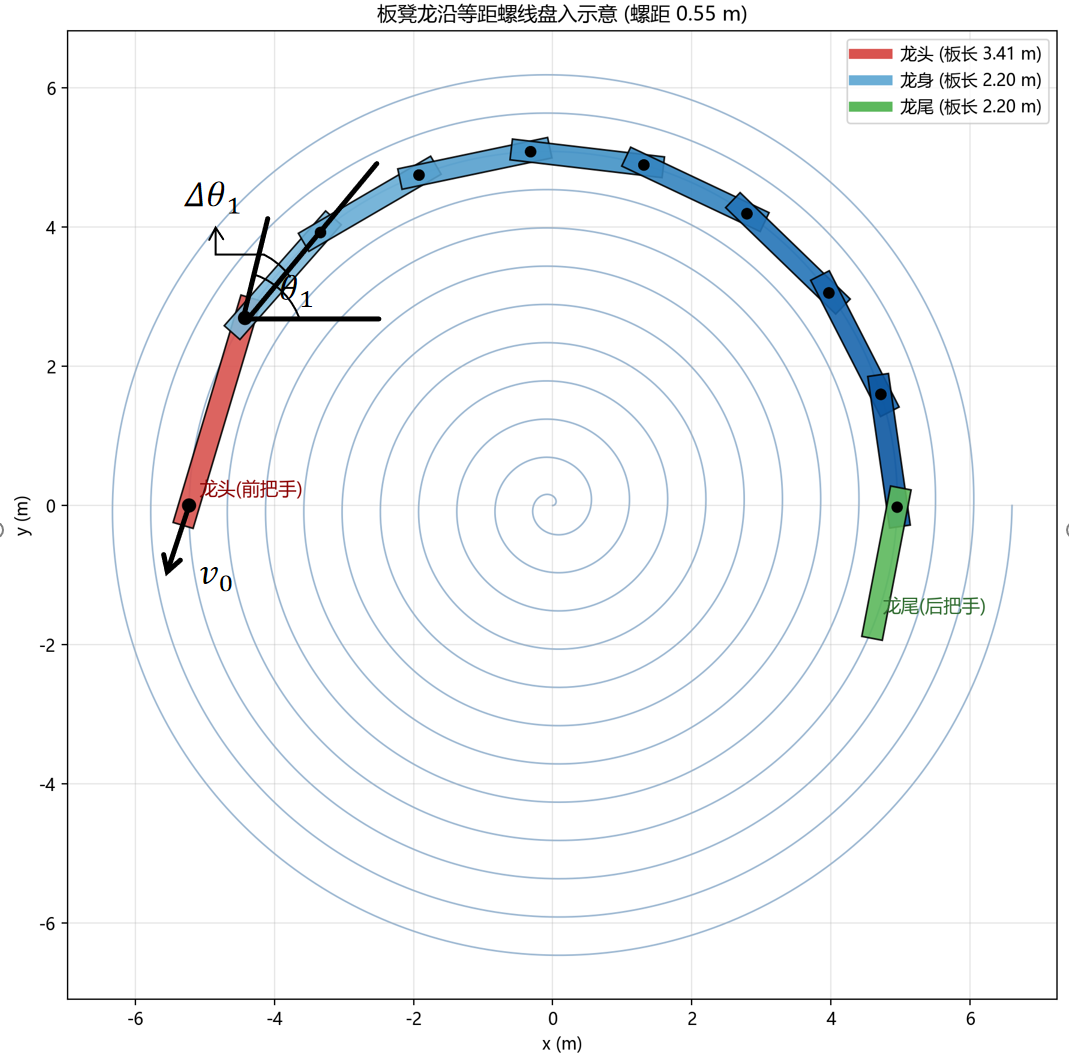
\includegraphics[width=0.49\textwidth]{figures/fig_盘入整体示意.png}
\caption{板凳龙沿等距螺线盘入整体示意（龙头＝红、龙身＝蓝、龙尾＝绿；$\theta_1$、$\Delta\theta_1$、$v_0$ 为关键几何量）}
\label{fig:spiral_overview}
\end{figure}

\subsubsection{板凳几何与相邻把手距离约束}
每节板凳前后各有一个孔径 $5.5\,\text{cm}$ 的把手孔，孔心距板端 $0.275\,\text{m}$（图~\ref{fig:bench_geo}）。相邻两节板凳通过把手在孔处铰接，故同一节板凳两孔中心的直线距离（有效杆长）为
\begin{equation}
L_1 = 3.41 - 2 \times 0.275 = 2.86\,\text{m}, \qquad
L_{body} = 2.20 - 2 \times 0.275 = 1.65\,\text{m},
\end{equation}
分别对应龙头与龙身、龙尾。这一刚体杆长不变约束与铰接车辆链条的相对运动规律一致~\cite{tanaka}：忽略把手间隙后，链条成为受螺线轨迹约束的刚性离散多体系统。

\begin{figure}[H]
\centering
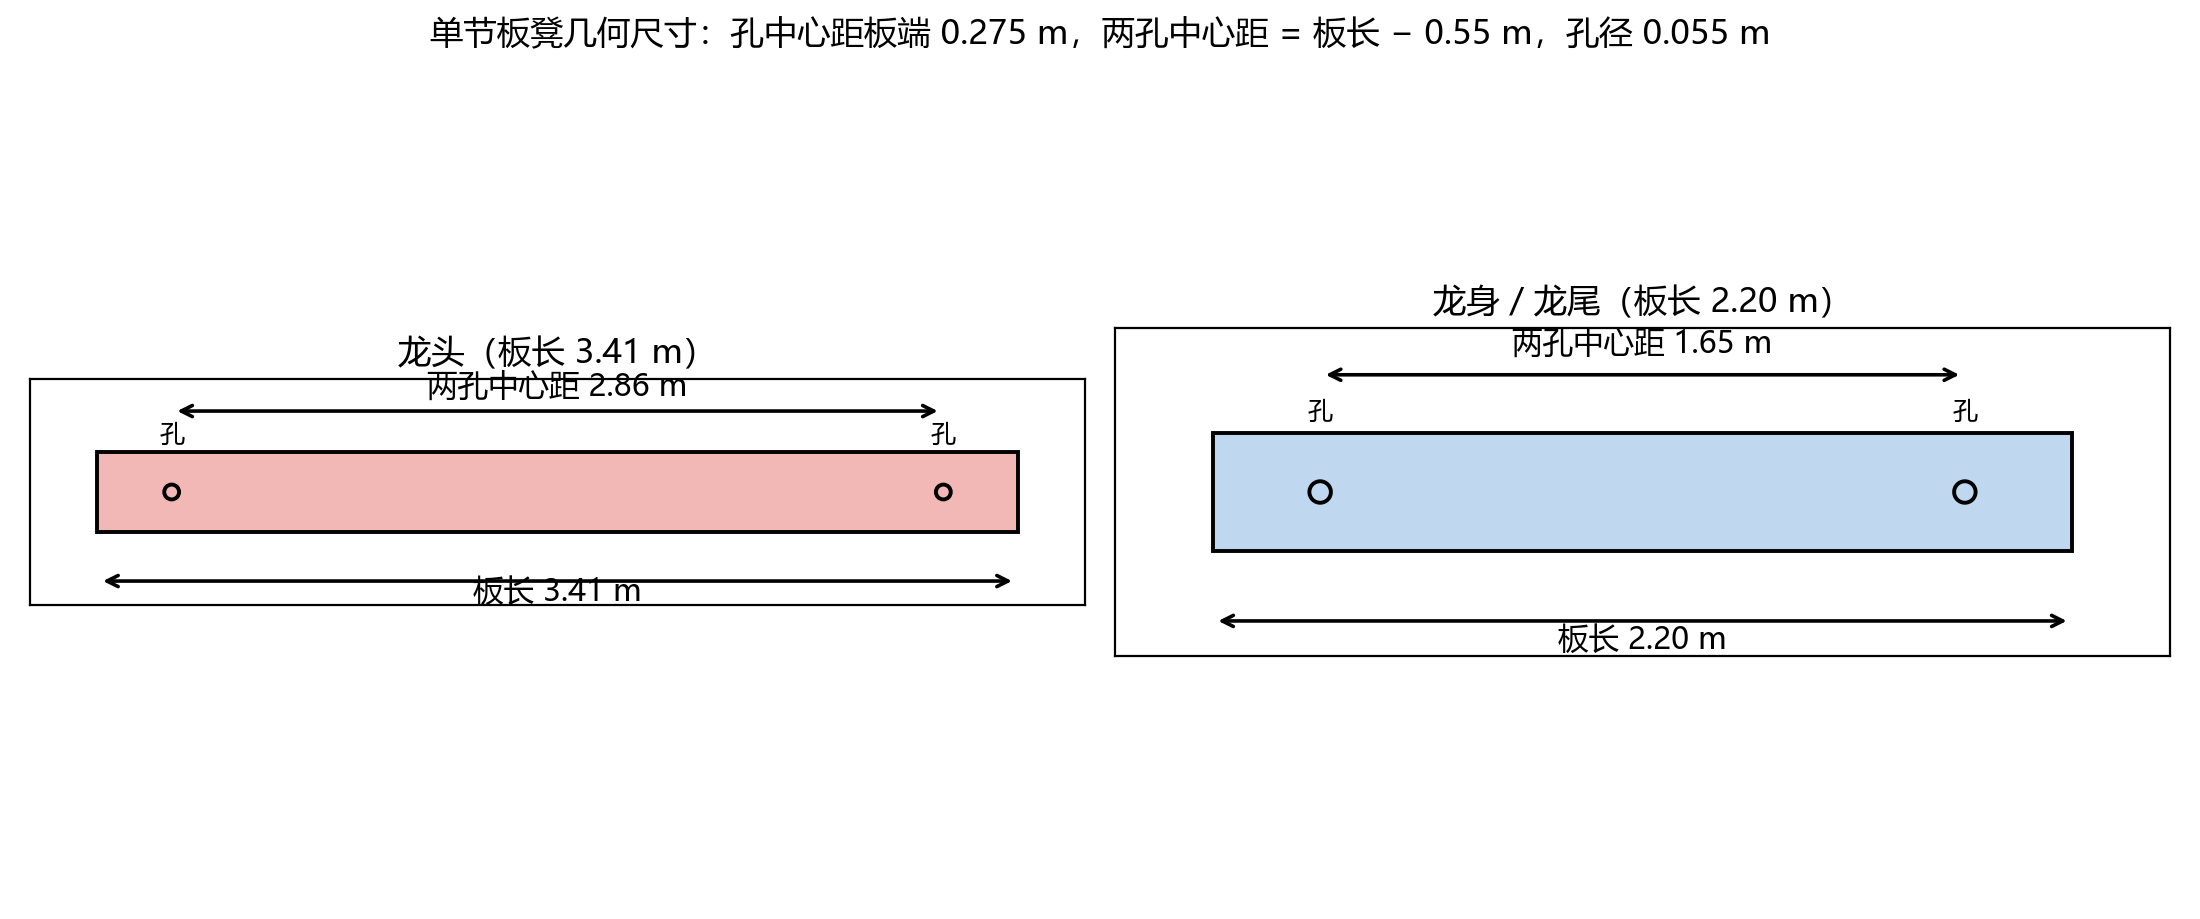
\includegraphics[width=0.64\textwidth]{figures/fig_板凳几何尺寸示意.png}
\caption{单节板凳几何尺寸示意（龙头板长 $3.41\,\text{m}$、龙身/龙尾板长 $2.20\,\text{m}$，两孔中心距分别为 $2.86\,\text{m}$ 与 $1.65\,\text{m}$）}
\label{fig:bench_geo}
\end{figure}

\subsubsection{几何逆推法求解各节点位置}
设把手沿链顺序编号 $P_1,P_2,\dots,P_{224}$（$P_1$ 为龙头前把手，$P_{224}$ 为龙尾后把手）。对任意节点 $i\ (i\ge 2)$，其位置须同时满足两个约束：一是该点落在螺线上，二是与前驱节点的直线距离等于有效杆长 $L_{i-1}$。联立得几何方程
\begin{equation}
\norm{\bm{P}_i(\theta_i) - \bm{P}_{i-1}(\theta_{i-1})}_2
= \sqrt{\left(b\theta_i\cos\theta_i - x_{i-1}\right)^2 + \left(b\theta_i\sin\theta_i - y_{i-1}\right)^2} = L_{i-1}.
\label{eq:recur}
\end{equation}
由于阿基米德螺线绕行多圈，以 $P_{i-1}$ 为圆心、$L_{i-1}$ 为半径的圆与螺线存在多个交点（图~\ref{fig:inversion}）。依据“龙头后方已盘过的螺线段上极角随半径增大而增大”的几何事实，取极角大于 $\theta_{i-1}$ 的交点中\textbf{极角最接近 $\theta_{i-1}$ 者}作为 $P_i$，即
\begin{equation}
\theta_i = \arg\min_{\theta\in\mathcal{S}}\ |\theta-\theta_{i-1}|,\qquad
\mathcal{S}=\{\theta>\theta_{i-1}:\ \norm{P(\theta)-P(\theta_{i-1})}=L_{i-1}\}.
\end{equation}
由于杆长（$1.65\sim2.86\,\text{m}$）远小于所在圈半径，方程~\eqref{eq:recur} 在 $\theta_{i-1}$ 的单侧邻域内恰有一根，用 Brent 求根算法可高效、稳定地逐节逆推出整条龙 224 个把手的空间坐标，相邻节点距离的数值误差不超过 $10^{-12}\,\text{m}$ 量级。

\begin{figure}[H]
\centering
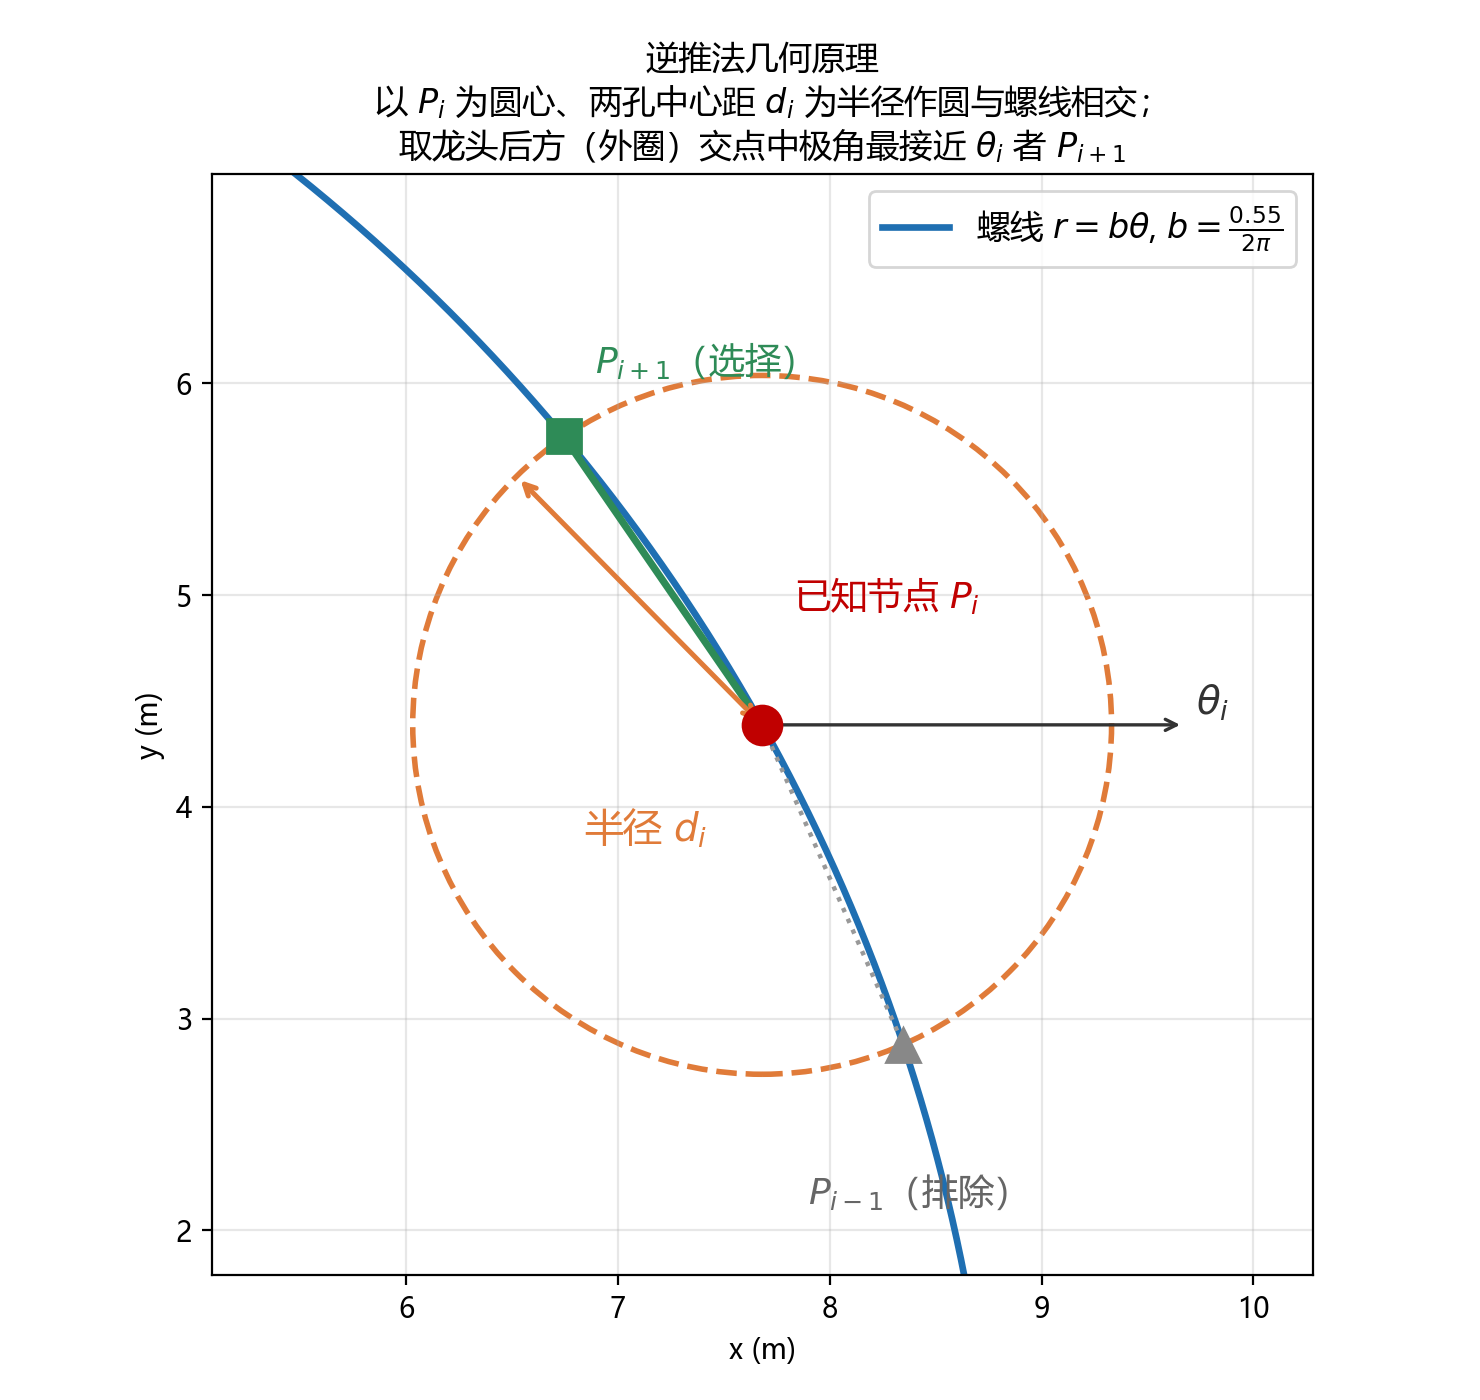
\includegraphics[width=0.47\textwidth]{figures/fig_逆推法几何示意.png}
\caption{几何逆推法原理：以已知把手为圆心、两孔中心距为半径作圆与已盘过螺线相交，取极角最接近的交点为下一节点}
\label{fig:inversion}
\end{figure}

\subsubsection{速度模型：中心差分与速度分解互验}
为求各节点瞬时速度，引入细步长时间微元 $\Delta t = 0.1\,\text{s}$，在离散位置序列上作二阶精度中心差分
\begin{equation}
v_i(t) \approx \frac{\norm{\bm{P}_i(t+\Delta t) - \bm{P}_i(t-\Delta t)}_2}{2\Delta t}.
\label{eq:diff}
\end{equation}
同时建立刚体铰接链的速度分解递推作为独立验证：各把手速度方向沿螺线单位切向量 $T(\theta)=\dfrac{\mathrm{d}P/\mathrm{d}\theta}{\norm{\mathrm{d}P/\mathrm{d}\theta}}$，杆两端沿杆方向的速度投影相等 $v_i\cdot e_i=v_{i+1}\cdot e_i$（$e_i$ 为杆方向单位向量），故
\begin{equation}
v_{i+1} = v_i\,\frac{T(\theta_i)\cdot e_i}{T(\theta_{i+1})\cdot e_i},
\qquad v_1 = 1\,\text{m/s}.
\end{equation}
两法结果最大相差约 $0.002\,\text{m/s}$，互相验证。这一“各把手弧长速率近似相同”的特征，与路径坐标参数化方法中沿给定路径传播速度的思想一致~\cite{verscheure,artunedo}。

\subsection{模型求解}

\subsubsection{求解算法流程}
问题一的求解流程为：对每个采样时刻，先二分求解弧长方程得龙头极角，再逐节 Brent 逆推全部把手位置，最后以细步长中心差分结合速度分解求出速度场，并对 $0\sim300\,\text{s}$ 全程执行实体碰撞检测（详见问题二判据）确认几何安全。

\subsubsection{求解结果}
按上述算法求得 $0\sim300\,\text{s}$ 每秒整条舞龙队 224 个把手的位置与速度（保留 6 位小数）并存入 \texttt{result1.xlsx}。论文要求的关键时刻位置与速度如表~\ref{tab:pos}、表~\ref{tab:vel} 所示。

\begin{table}[H]
\centering
\caption{各关键时刻全部指定把手的位置（单位：m）}
\label{tab:pos}
\scriptsize\setlength{\tabcolsep}{3.6pt}
\renewcommand{\arraystretch}{1.08}
\begin{tabular}{lrrrrrr}
\toprule
 & 0 s & 60 s & 120 s & 180 s & 240 s & 300 s \\
\midrule
龙头 $x$ & 8.800000 & 5.799209 & $-4.084887$ & $-2.963609$ & 2.594494 & 4.420274 \\
龙头 $y$ & 0.000000 & $-5.771092$ & $-6.304479$ & 6.094780 & $-5.356743$ & 2.320429 \\
第 1 节龙身 $x$ & 8.363824 & 7.456758 & $-1.445473$ & $-5.237118$ & 4.821221 & 2.459489 \\
第 1 节龙身 $y$ & 2.826544 & $-3.440399$ & $-7.405883$ & 4.359627 & $-3.561949$ & 4.402476 \\
第 51 节龙身 $x$ & $-9.518732$ & $-8.686317$ & $-5.543150$ & 2.890455 & 5.980011 & $-6.301346$ \\
第 51 节龙身 $y$ & 1.341137 & 2.540108 & 6.377946 & 7.249289 & $-3.827758$ & 0.465829 \\
第 101 节龙身 $x$ & 2.913983 & 5.687116 & 5.361939 & 1.898794 & $-4.917371$ & $-6.237722$ \\
第 101 节龙身 $y$ & $-9.918311$ & $-8.001384$ & $-7.557638$ & $-8.471614$ & $-6.379874$ & 3.936008 \\
第 151 节龙身 $x$ & 10.861726 & 6.682311 & 2.388757 & 1.005154 & 2.965378 & 7.040740 \\
第 151 节龙身 $y$ & 1.828753 & 8.134544 & 9.727411 & 9.424751 & 8.399721 & 4.393013 \\
第 201 节龙身 $x$ & 4.555102 & $-6.619664$ & $-10.627211$ & $-9.287720$ & $-7.457151$ & $-7.458662$ \\
第 201 节龙身 $y$ & 10.725118 & 9.025570 & 1.359847 & $-4.246673$ & $-6.180726$ & $-5.263384$ \\
龙尾（后）$x$ & $-5.305444$ & 7.364557 & 10.974348 & 7.383896 & 3.241051 & 1.785033 \\
龙尾（后）$y$ & $-10.676584$ & $-8.797992$ & 0.843473 & 7.492370 & 9.469336 & 9.301164 \\
\bottomrule
\end{tabular}
\end{table}

\begin{table}[H]
\centering
\caption{各关键时刻全部指定把手的速度（单位：m/s）}
\label{tab:vel}
\scriptsize\setlength{\tabcolsep}{3.6pt}
\renewcommand{\arraystretch}{1.08}
\begin{tabular}{lrrrrrr}
\toprule
 & 0 s & 60 s & 120 s & 180 s & 240 s & 300 s \\
\midrule
龙头 & 0.999995 & 0.999975 & 0.999970 & 0.999964 & 0.999953 & 0.999983 \\
第 1 节龙身 & 0.999966 & 0.999936 & 0.999916 & 0.999881 & 0.999812 & 0.999693 \\
第 51 节龙身 & 0.999737 & 0.999642 & 0.999515 & 0.999303 & 0.998908 & 0.998055 \\
第 101 节龙身 & 0.999571 & 0.999436 & 0.999250 & 0.998949 & 0.998410 & 0.997296 \\
第 151 节龙身 & 0.999444 & 0.999284 & 0.999061 & 0.998709 & 0.998094 & 0.996857 \\
第 201 节龙身 & 0.999345 & 0.999167 & 0.998920 & 0.998535 & 0.997876 & 0.996571 \\
龙尾（后） & 0.999308 & 0.999124 & 0.998869 & 0.998474 & 0.997800 & 0.996475 \\
\bottomrule
\end{tabular}
\end{table}

图~\ref{fig:traj} 给出 $t=0,60,\dots,300\,\text{s}$ 六个时刻整条龙在螺线上的形态叠加：龙头自第 16 圈起点 $(8.8,0)$ 顺时针持续盘入，全链 224 个把手严格落于螺线。图~\ref{fig:head_rtheta} 显示龙头极径 $r(t)$ 单调递减、极角 $\theta(t)$ 单调递减，符合顺时针盘入的运动方向，直角坐标分量则呈现螺线运动的周期特征。图~\ref{fig:vel} 表明全链各把手速度稳定在 $1\,\text{m/s}$ 附近（$0.996\sim1.000\,\text{m/s}$），龙尾后把手极径随盘入同步收拢，与“刚性链沿固定螺线无伸长滑移”的物理预期一致。整条盘入过程的动态仿真见电子附件动画。

\begin{figure}[H]
\centering
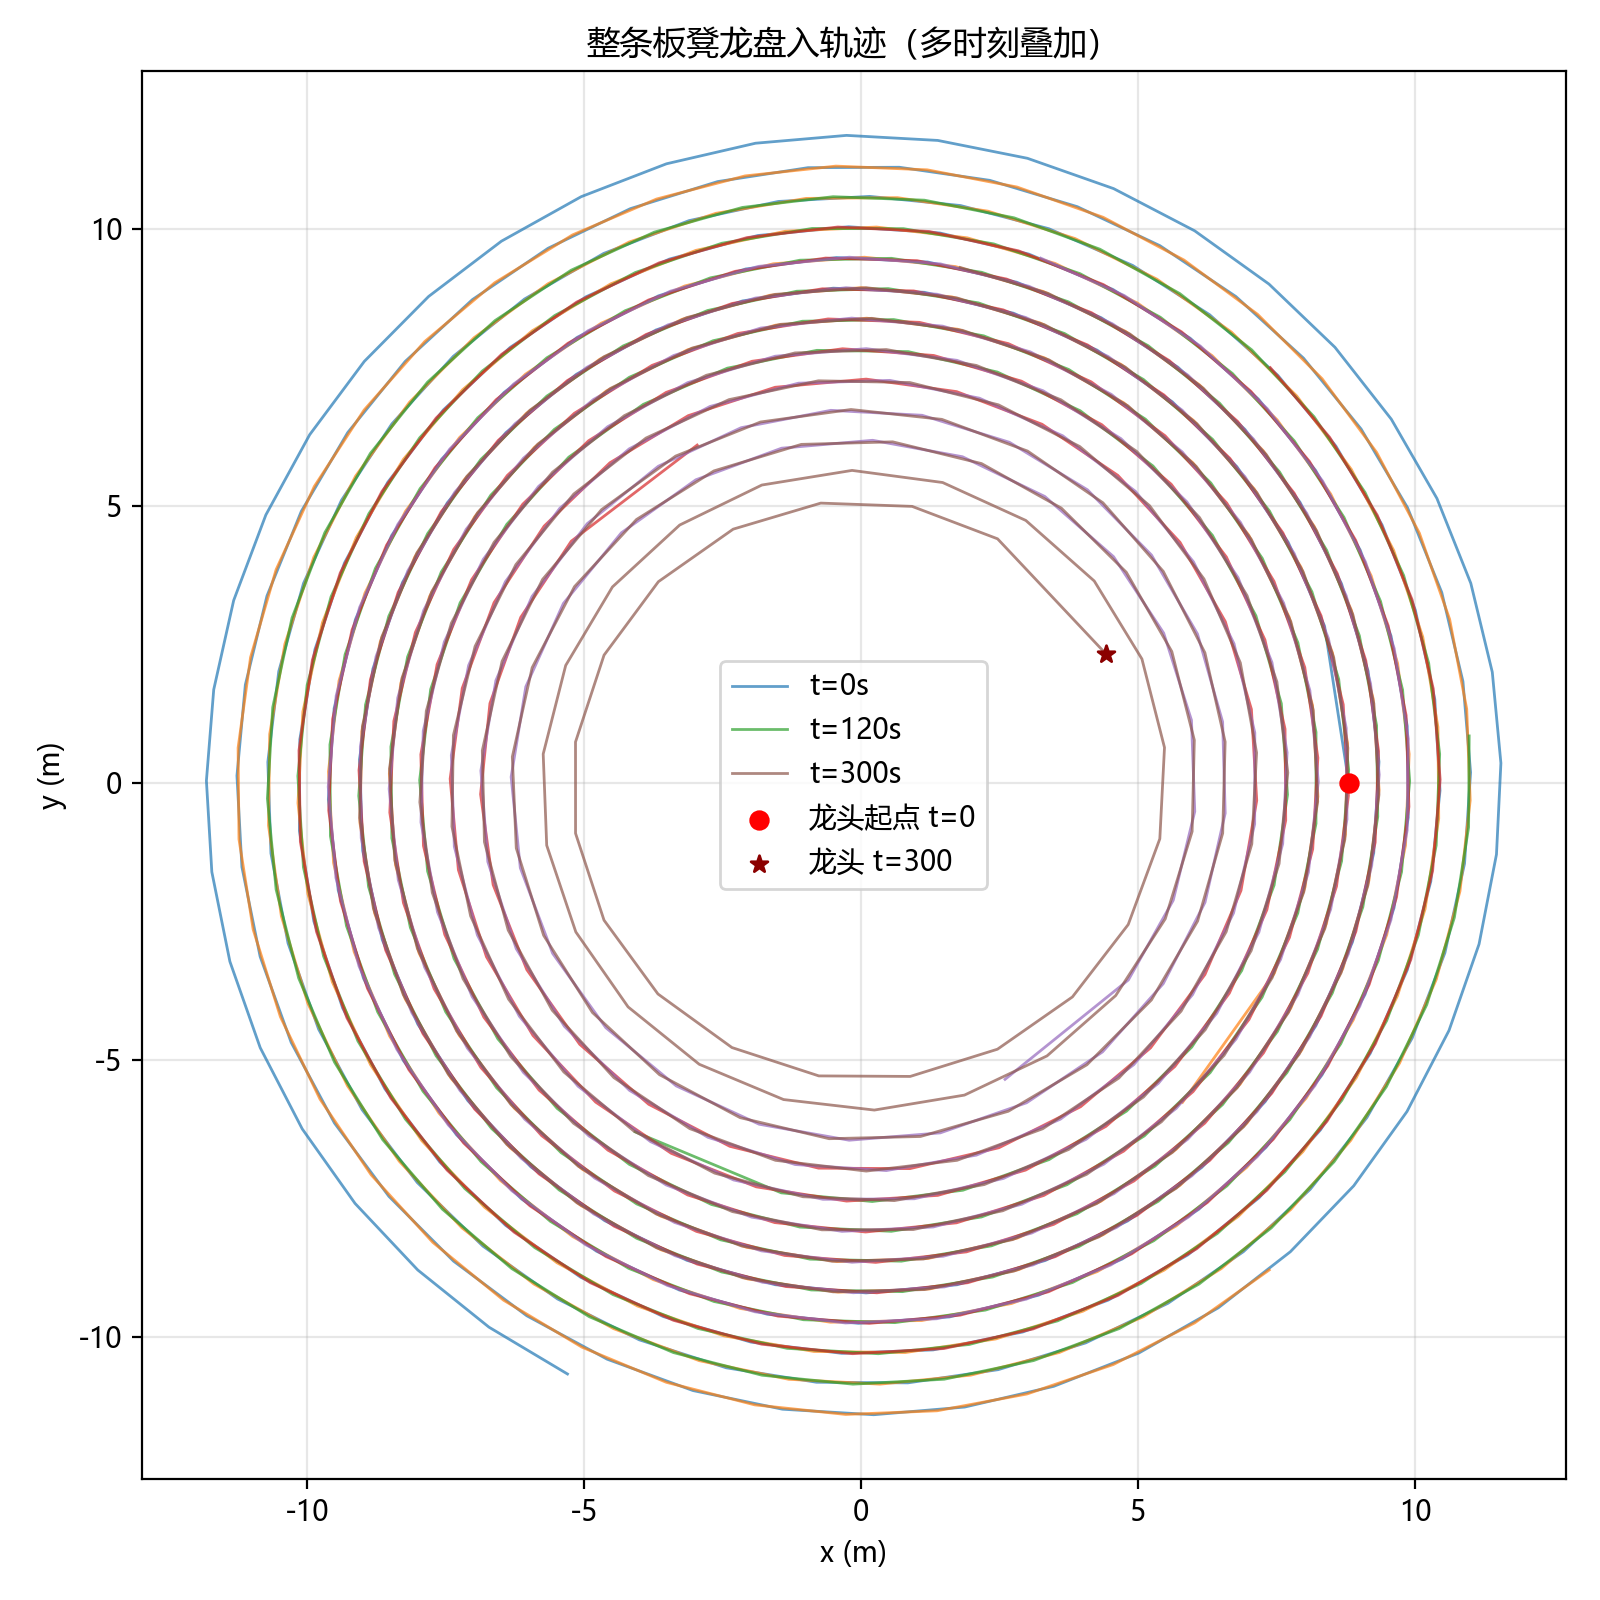
\includegraphics[width=0.455\textwidth]{figures/fig_整龙盘入轨迹.png}
\caption{$t=0,60,\dots,300\,\text{s}$ 整条板凳龙盘入轨迹叠加图}
\label{fig:traj}
\end{figure}

\begin{figure}[H]
\centering
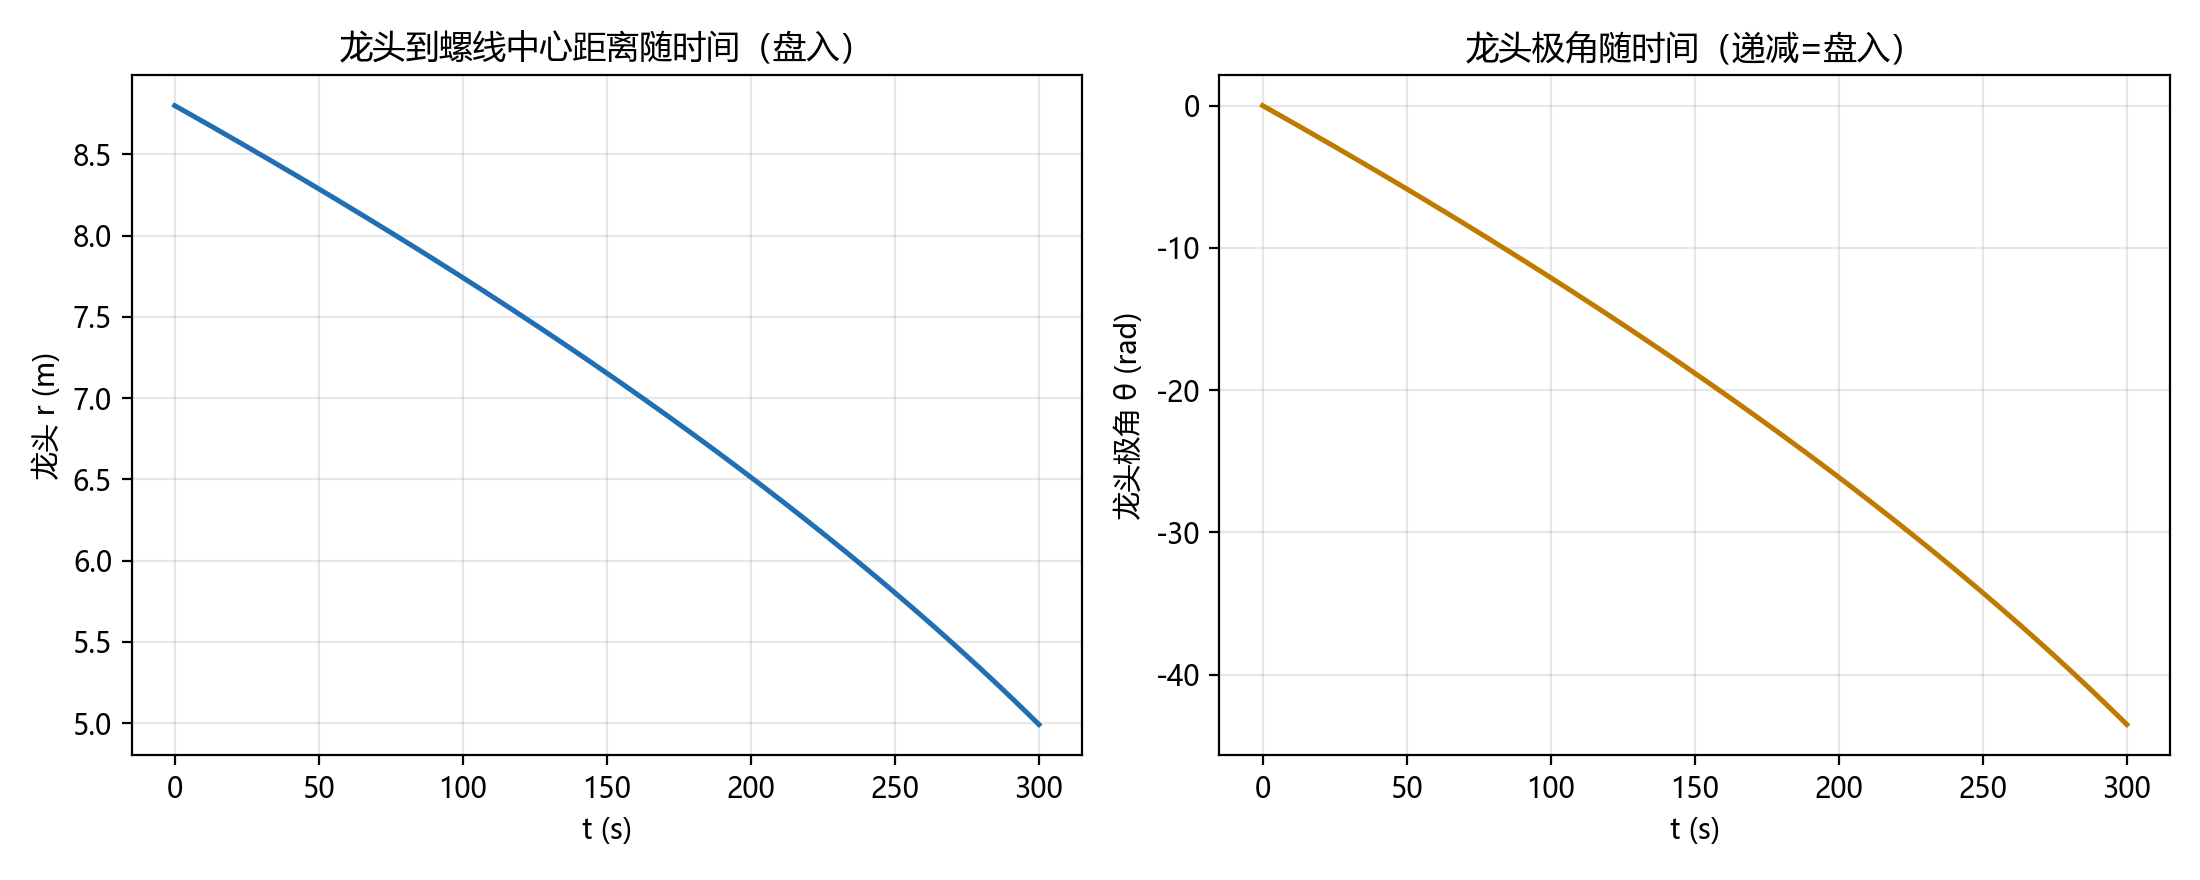
\includegraphics[width=0.61\textwidth]{figures/fig_龙头半径角度随时间.png}
\caption{龙头到螺线中心的距离（左）与极角（右）随时间变化}
\label{fig:head_rtheta}
\end{figure}

\begin{figure}[H]
\centering
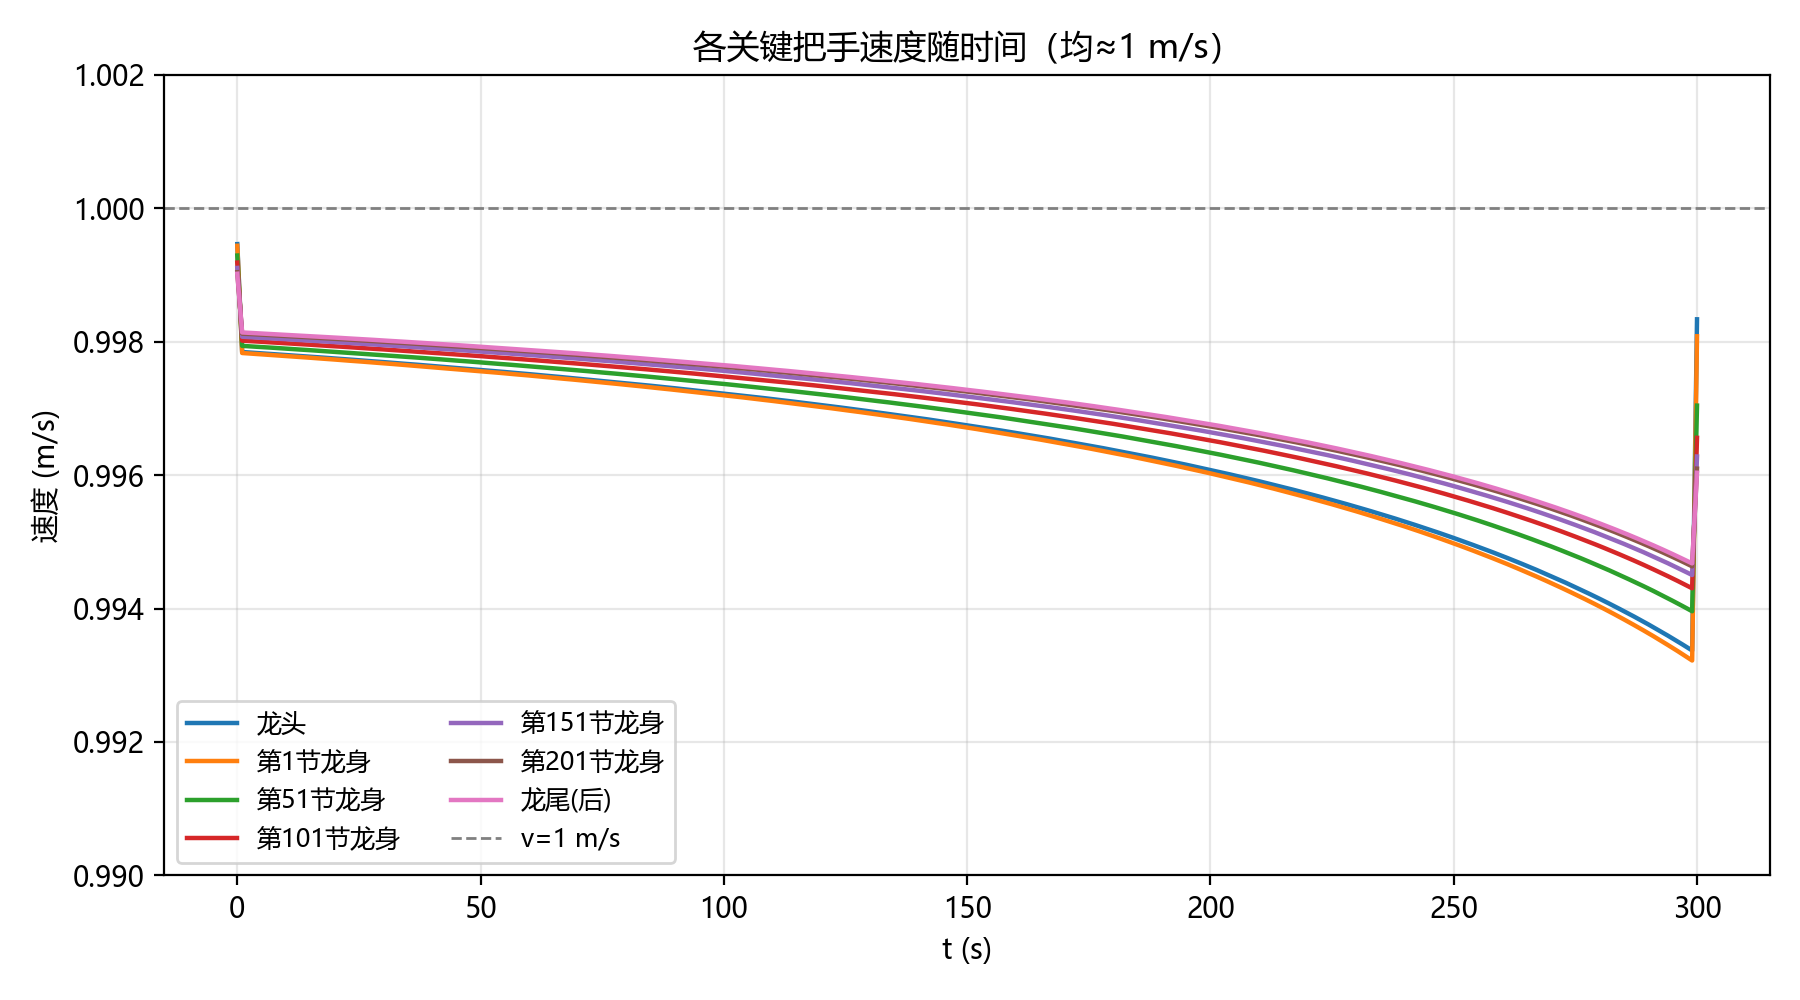
\includegraphics[width=0.612\textwidth]{figures/fig_把手速度随时间.png}
\caption{龙头及第 $1/51/101/151/201$ 节龙身、龙尾后把手速度随时间变化（均 $\approx 1\,\text{m/s}$）}
\label{fig:vel}
\end{figure}

\subsubsection{实体碰撞检测与合理性验证}
以板宽 $0.30\,\text{m}$ 将每节板凳实体化为旋转矩形，对全部非相邻板凳对执行分离轴检测（判据见第六章），得 $0\sim300\,\text{s}$ 全程最小间隙为 $1.95\times10^{-7}\,\text{m}>0$，即问题一时间域内盘入全程无碰撞；该最小间隙出现在第 73 节与第 166 节之间，系相邻螺线圈板体斜向逼近所致，说明该螺距下系统已处于“紧致但安全”的临界状态。相邻把手距离全量校验误差不超过 $5\times10^{-7}\,\text{m}$（6 位小数舍入），与问题二的碰撞终止时刻 $t^{*}$ 相互印证。

\section{问题二模型的建立和求解}

\subsection{模型建立}

\subsubsection{板凳实体的旋转矩形建模}
碰撞的物理本质是板体的几何干涉，而非把手点的重合。将第 $i$ 节板凳建模为平面旋转矩形：以两把手中心 $P_i,P_{i+1}$ 的中点 $C_i$ 为中心、沿杆方向单位向量 $u_i$ 为长轴，半长为 $L_i/2$（$L_i$ 为板长）、半宽为板宽之半 $w/2=0.15\,\text{m}$，其四顶点为 $C_i\pm \frac{L_i}{2}u_i\pm\frac{w}{2}n_i$（$n_i$ 为单位法向）。值得注意的是，铰接链条中相邻节相对转角过大同样会导致板体重叠（“折刀”现象）~\cite{tanaka}；后文数值结果表明本问题盘入全程相邻板凳夹角最小约 $7.9^\circ$、无折刀风险，故碰撞判据针对非相邻板凳建立。

\subsubsection{混合干涉判据：分离轴定理与顶点包容}
碰撞判定即两旋转矩形是否相交。仅检测边—边交点存在退化漏检：当一狭长矩形完全落入另一矩形内部时，两边界无任何交点，但实际已发生干涉（图~\ref{fig:rect_cases} 中）。为此建立混合判据：
\begin{enumerate}
    \item \textbf{分离轴定理（SAT）}：将两矩形分别向共计 4 个法向轴投影。若存在某一轴使投影区间分离，则两矩形必不相交；若 4 轴投影全部重叠，则判定相交。SAT 对凸多边形成立，天然覆盖“完全包含”情形；
    \item \textbf{顶点包容检验}：检验矩形 $A$ 的 4 个顶点是否落入矩形 $B$ 内部（反之亦然），作为退化包含情形的双重防线。
\end{enumerate}
两判据取并，任一成立即判碰撞，保证判定的完备性。

\begin{figure}[H]
\centering
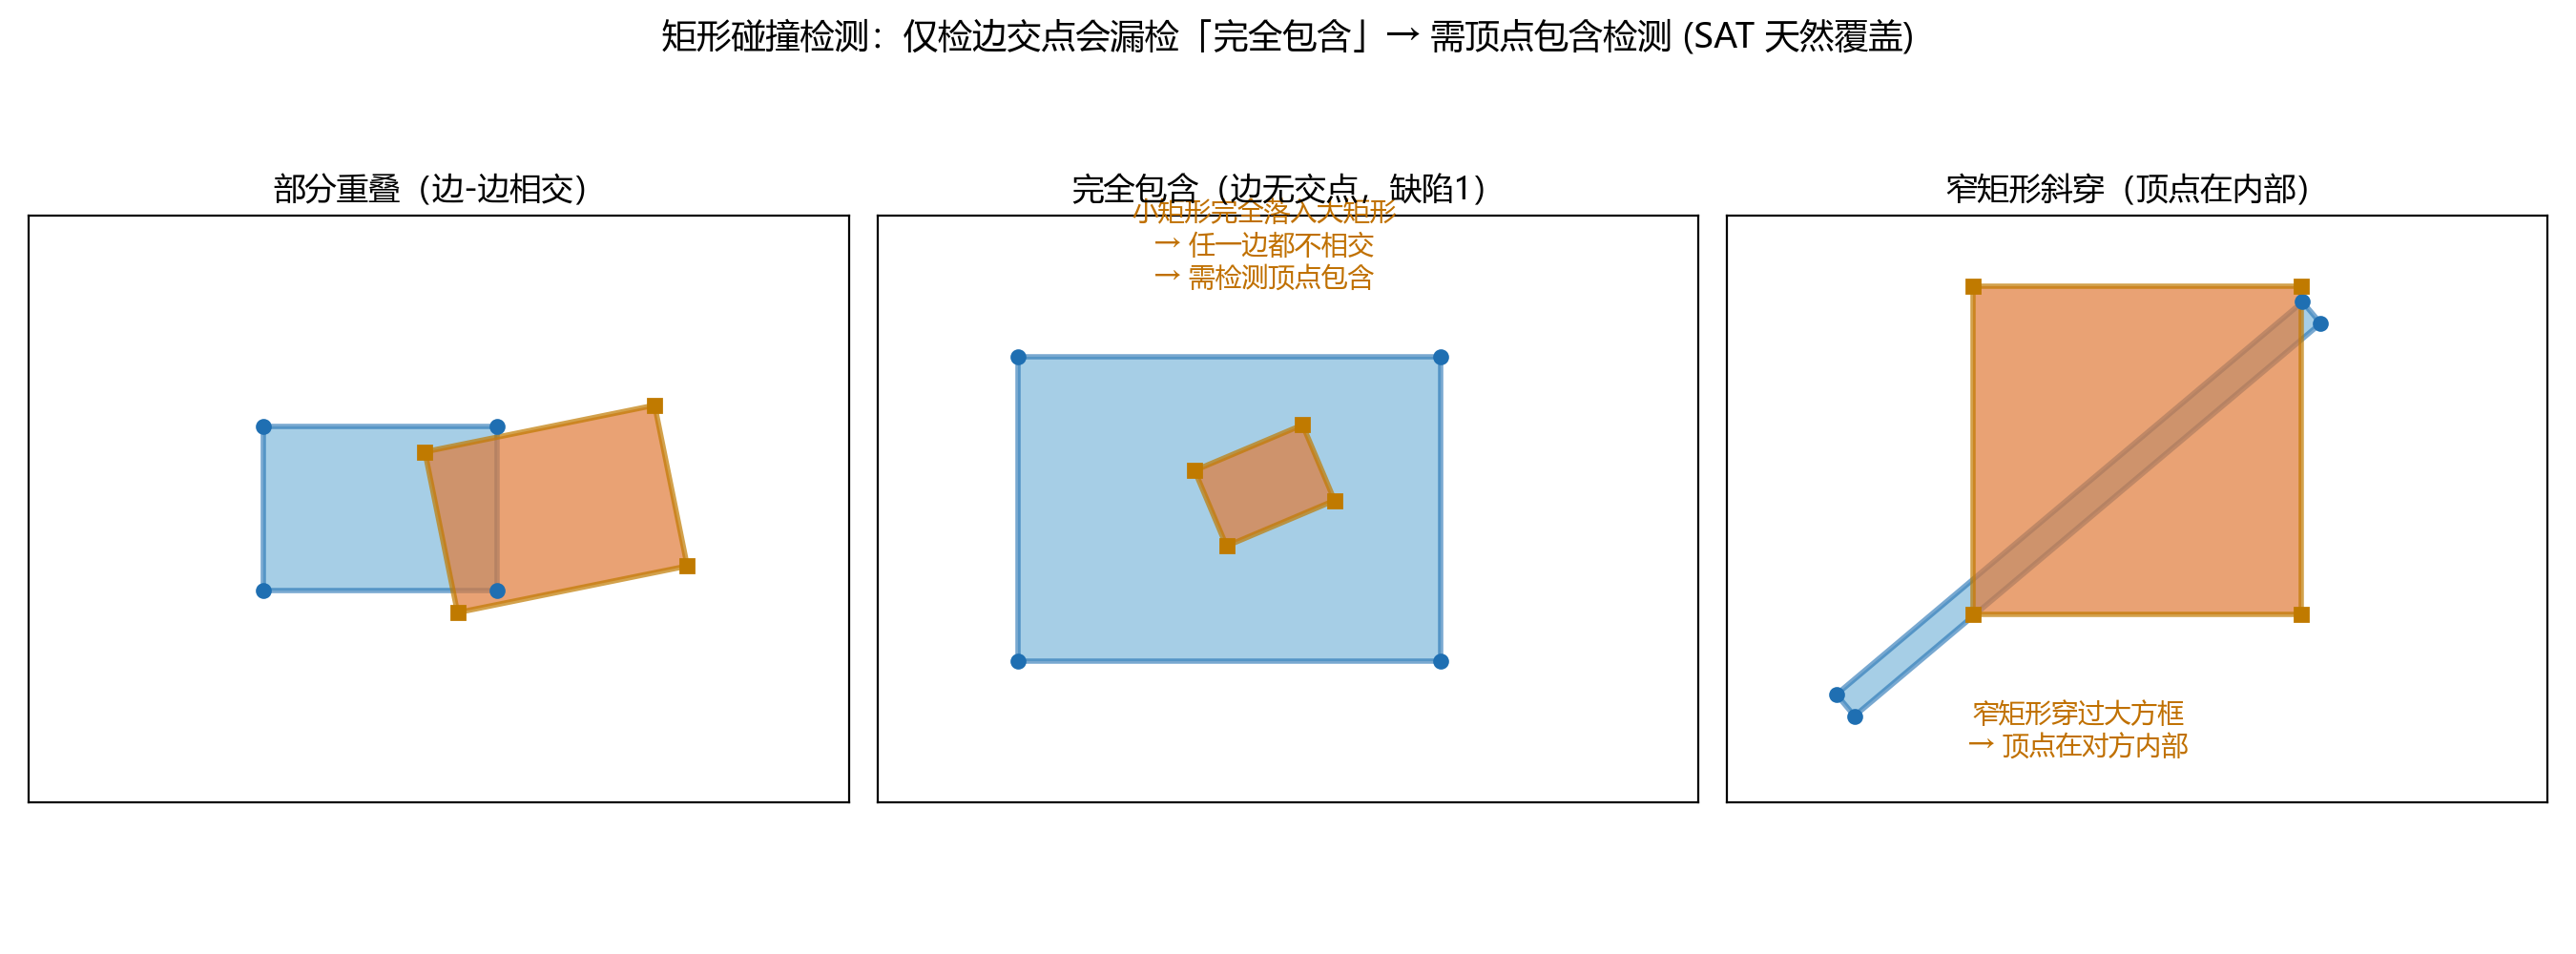
\includegraphics[width=0.70\textwidth]{figures/fig_矩形碰撞示意.png}
\caption{矩形碰撞的三种典型情形：部分重叠（左）、完全包含（中，仅检边交点将漏检）、窄矩形斜穿（右，顶点落入对方内部）}
\label{fig:rect_cases}
\end{figure}

\subsubsection{宽相预筛与计算复杂度控制}
$223$ 节板凳两两组合共 $\binom{223}{2}=24753$ 对，若对每对均作精判则开销较大。为此先作宽相筛选：对每节板凳计算其外接轴向包围盒（AABB），半宽为
\begin{equation}
e_x=\tfrac{L}{2}|u_x|+\tfrac{w}{2}|n_x|,\qquad
e_y=\tfrac{L}{2}|u_y|+\tfrac{w}{2}|n_y|.
\end{equation}
若两 AABB 在 $x$ 或 $y$ 方向投影区间分离，则对应板凳对必然不相交，直接跳过精判；仅对 AABB 可能重叠的候选对执行“顶点包容 $\cup$ SAT”精判。该两阶段策略使单时刻检测的开销大幅下降。

\subsection{模型求解}

\subsubsection{带符号间隙函数与连续碰撞检测}
固定时间步长的离散扫描存在“隧道效应”：两矩形在区间端点均分离、却在区间中途短暂重叠时将被漏检。为消除该误差，定义两节板凳间的\textbf{带符号间隙函数}
\begin{equation}
g(t)=
\begin{cases}
\displaystyle\min_{\text{分离轴}}\bigl(\text{投影分离量}\bigr), & \text{不相交（分离）},\\[4pt]
-\displaystyle\max_{\text{重叠轴}}\bigl(\text{投影重叠深度}\bigr), & \text{相交（碰撞）}.
\end{cases}
\end{equation}
$g(t)>0$ 表示分离、$g(t)\le 0$ 表示碰撞，且与精相判定完全一致。在可疑时间子区间 $[t_a,t_b]$ 内，用黄金分割法搜索 $g(t)$ 的最小值：
\begin{equation}
\min_{t \in [t_a, t_b]} g(t).
\end{equation}
若该极小值小于零，则证明区间内发生过碰撞，从而在机制上保证不因步长离散而漏检（图~\ref{fig:ccd}）。

\begin{figure}[H]
\centering
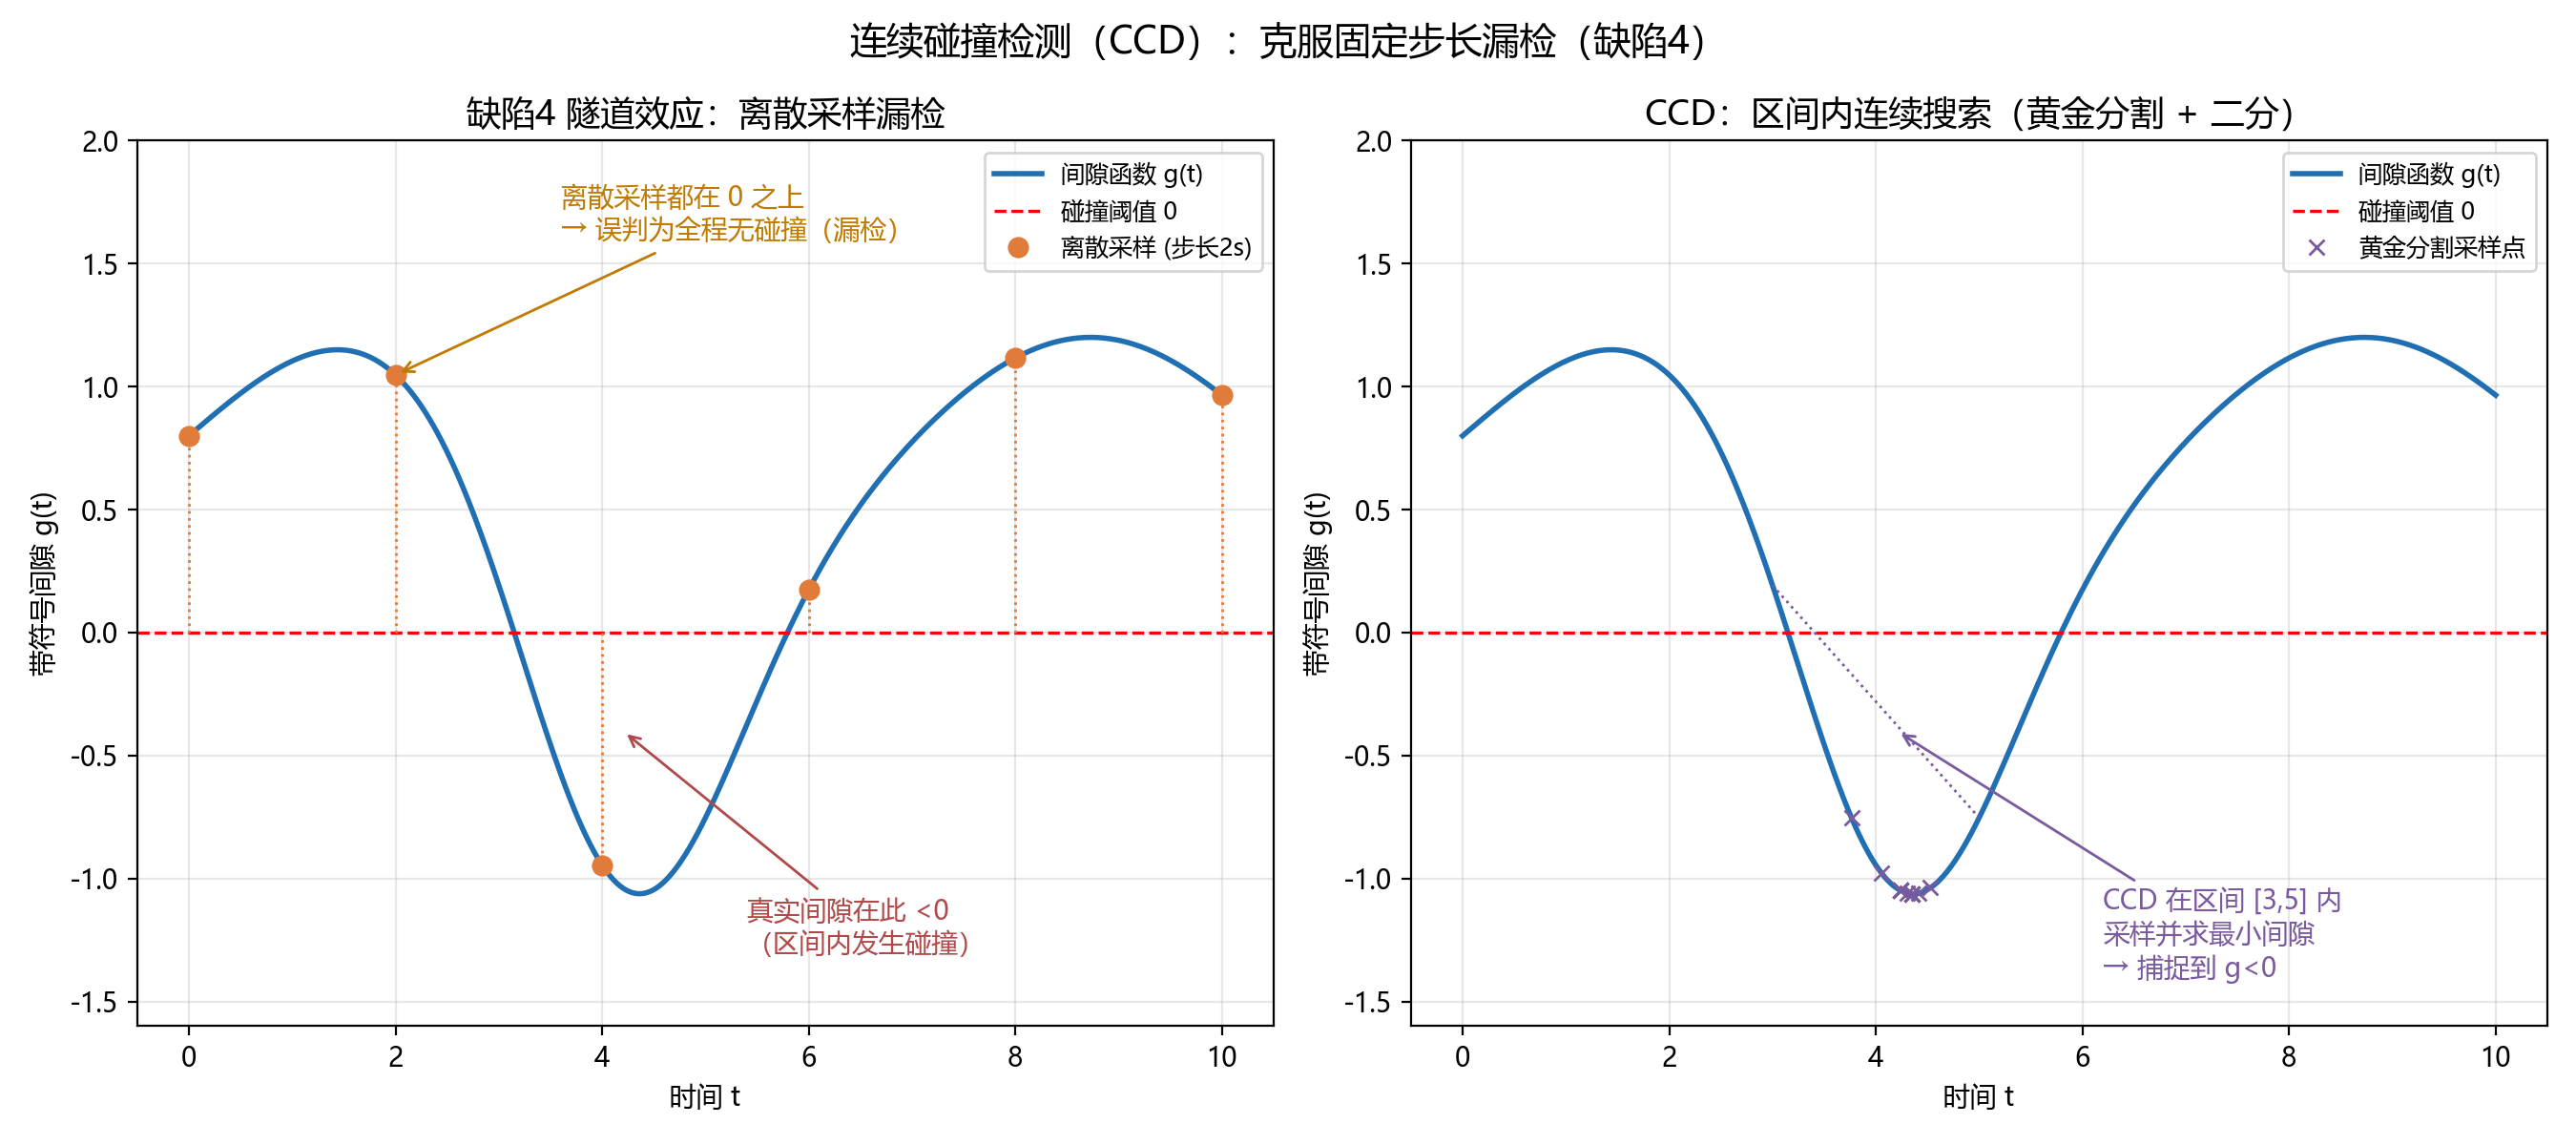
\includegraphics[width=0.70\textwidth]{figures/fig_CCD连续碰撞示意.png}
\caption{连续碰撞检测（CCD）：左为隧道效应导致离散采样漏检，右为 CCD 在区间内以黄金分割捕捉 $g<0$}
\label{fig:ccd}
\end{figure}

\subsubsection{二分法逼近终止时刻}
整体求解流程为：外层先以大步长扫描定位首个碰撞区间 $[t_{lo},t_{hi}]$（$t_{lo}$ 无碰撞、$t_{hi}$ 有碰撞），再以二分法收缩区间
\begin{equation}
t_{mid}=\frac{t_{lo}+t_{hi}}{2},\qquad
\text{若 } g(t_{mid})\le 0 \text{ 则 } t_{hi}=t_{mid},\ \text{否则 } t_{lo}=t_{mid},
\end{equation}
直至区间宽度小于 $10^{-3}\,\text{s}$，并以 CCD 黄金分割在临界区间内连续精化，得到“恰发生碰撞”的终止时刻 $t^{*}$。

\subsubsection{求解结果}
经计算，盘入的安全终止时刻为
\begin{equation}
t^{*} = 412.47\,\text{s},
\end{equation}
首次发生干涉的板凳对为\textbf{第 1 节（龙头）}与\textbf{第 9 节}板身。其力学成因是：临界时刻龙头位于内圈（极径 $r\approx 2.26\,\text{m}$，约第 4 圈），而第 9 节板凳位于相邻外圈（极径约 $2.80\,\text{m}$，约第 5 圈），两板中心相距仅约 $1.25\,\text{m}$，小于板长量级，板体在相邻螺线圈间发生径向干涉。数值验证显示重叠深度在 $t=412.47\,\text{s}$ 附近由负单调过零，二分与 CCD 给出的接触时刻一致到毫秒级。

终止时刻 $t^{*}$ 整条舞龙队的位置与速度已存入 \texttt{result2.xlsx}，关键把手状态如表~\ref{tab:tstar} 所示；临界时刻全龙形态见图~\ref{fig:collision_view}，可见碰撞对位于螺线内圈、其余部分仍沿外圈规则展开。

\begin{table}[H]
    \centering
    \caption{终止时刻 $t^* = 412.47\,\text{s}$ 各关键把手的空间状态表}
    \label{tab:tstar}
    \begin{tabular}{lccc}
        \toprule
        节点名称 & X 坐标 (m) & Y 坐标 (m) & 瞬时速度 (m/s) \\
        \midrule
        龙头 (前把手) & 1.206828 & 1.944881 & 1.000000 \\
        第 1 节龙身 (前把手) & $-1.646589$ & 1.750958 & 0.991553 \\
        第 51 节龙身 (前把手) & 1.277714 & 4.327693 & 0.976863 \\
        第 101 节龙身 (前把手) & $-0.532617$ & $-5.880522$ & 0.974555 \\
        第 151 节龙身 (前把手) & 0.972457 & $-6.957020$ & 0.973613 \\
        第 201 节龙身 (前把手) & $-7.892638$ & $-1.234370$ & 0.973101 \\
        龙尾 (后把手) & 0.952602 & 8.323189 & 0.972943 \\
        \bottomrule
    \end{tabular}
\end{table}

\begin{figure}[H]
\centering
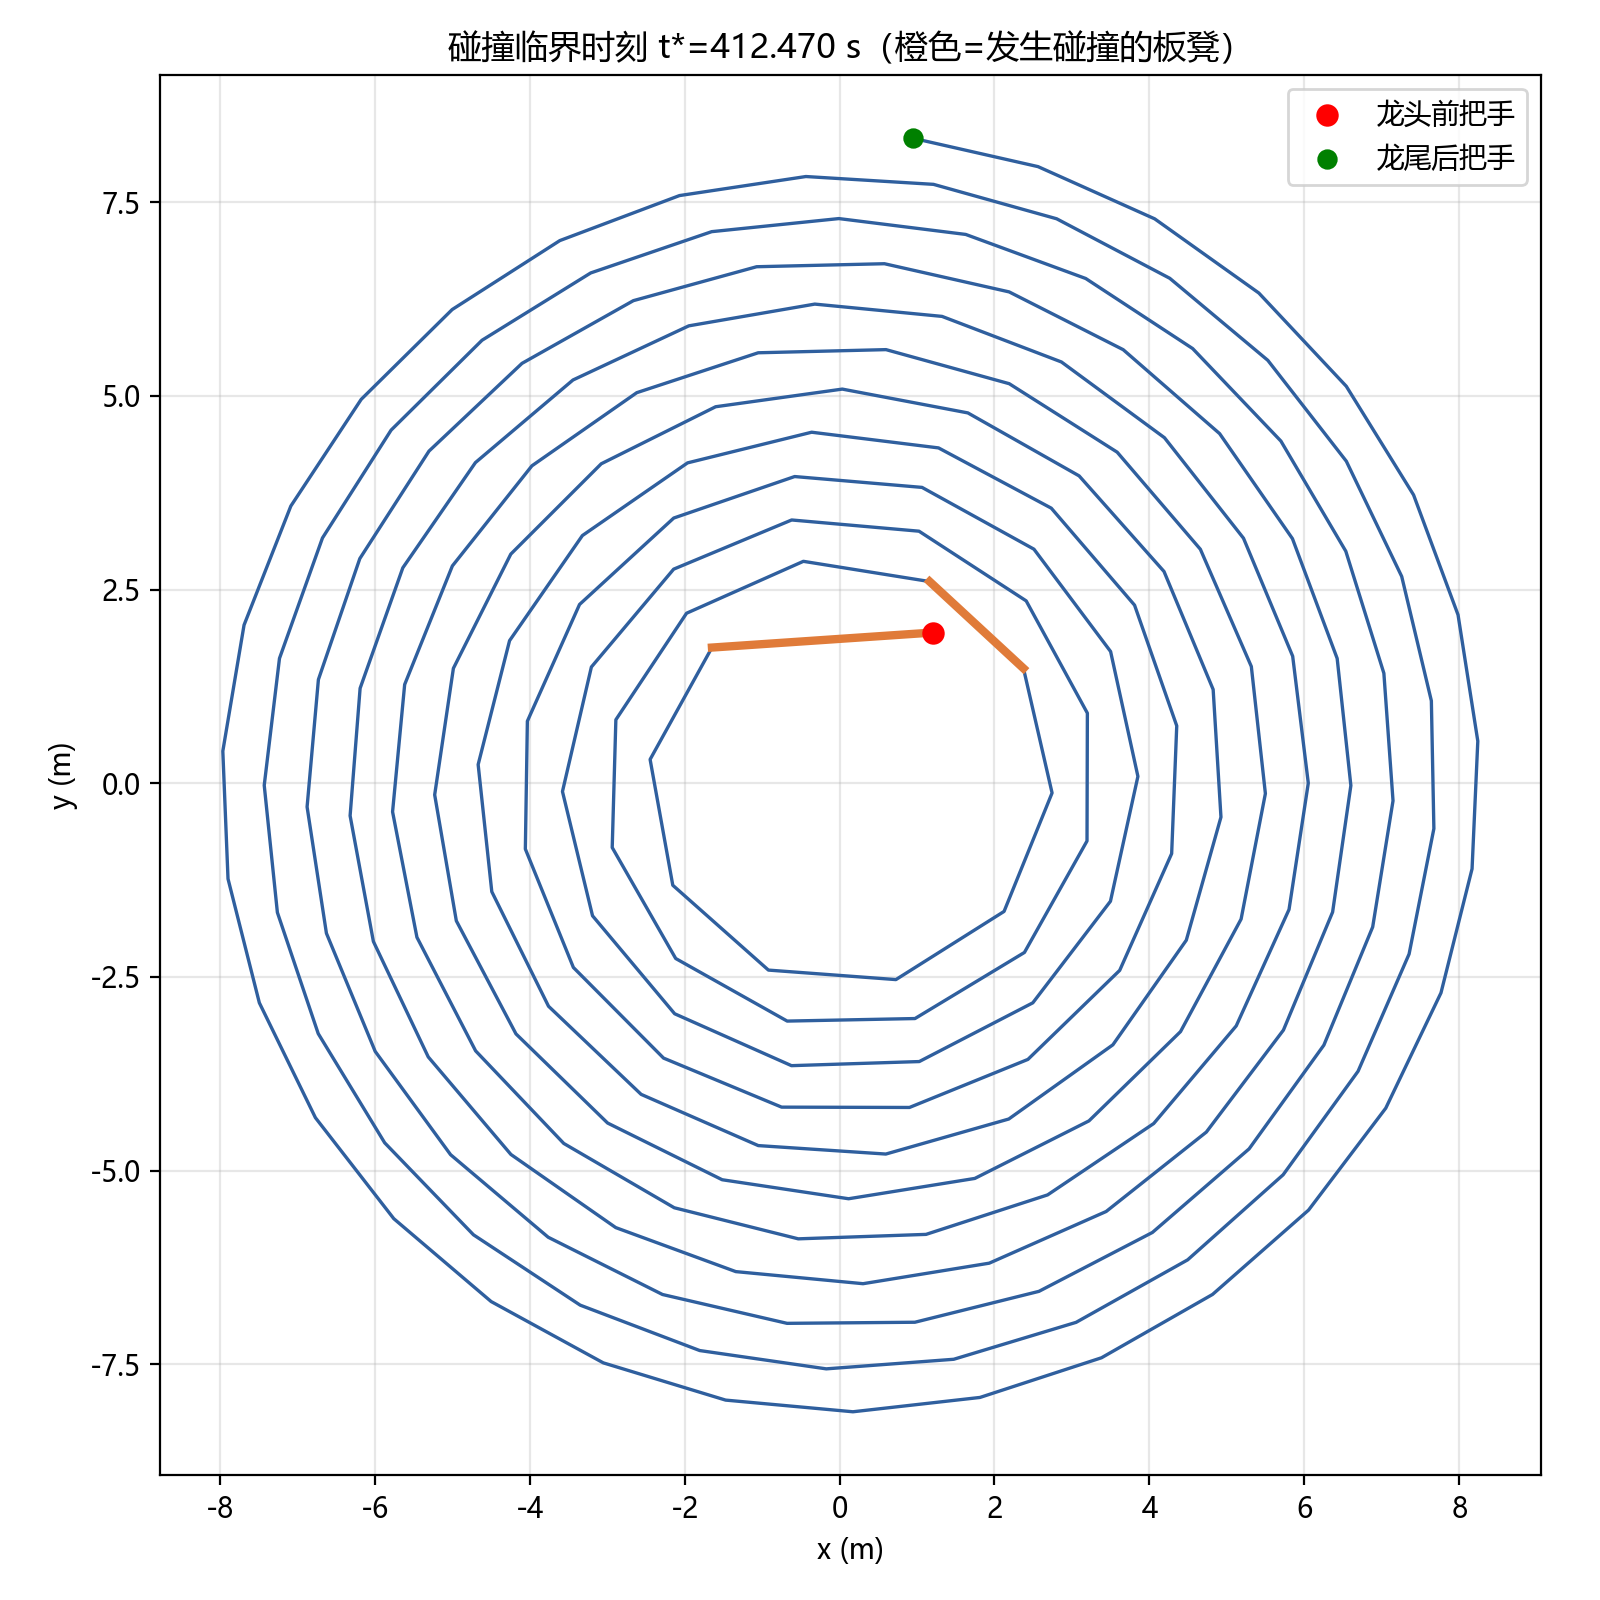
\includegraphics[width=0.52\textwidth]{figures/fig_碰撞临界时刻.png}
\caption{干涉临界时刻（$t^{*}=412.47\,\text{s}$）全龙形态（橙色为发生干涉的板凳对：龙头与第 9 节）}
\label{fig:collision_view}
\end{figure}

\section{问题三模型的建立和求解}

\subsection{模型建立}

\subsubsection{螺距参数化的螺线族与决策变量}
与问题一、二不同，问题三中螺线本身待定：每给定一个螺距 $p$，即确定一条螺线 $r(\theta)=b\theta$（$b=p/2\pi$）以及沿该螺线的一整族盘入构型。初始条件与问题一一致：龙头前把手位于第 16 圈，$\theta_0=32\pi$、$r_0=16p$，并以 $v_0=1\,\text{m/s}$ 顺时针盘入。决策变量取
\begin{equation}
p \in [\,0.30,\ 1.70\,]\,\text{m},
\end{equation}
下界取板宽 $0.30\,\text{m}$（更小的螺距下相邻圈间隙不足以容纳一块板凳，必然碰撞），上界取题设参考螺距 $1.7\,\text{m}$。由于任意时刻全部把手位置由“龙头已走过的弧长”唯一决定，碰撞可行性与行进速度大小无关，$p^{*}$ 是纯几何量，优化模型为
\begin{equation}
\min_{p}\ p \qquad
\text{s.t.}\quad
\begin{cases}
\text{（几何）} & \norm{P(\theta_{i+1})-P(\theta_i)}=L_i,\ \ \theta_i\ \text{逐节递推},\\
\text{（边界）} & r(\theta_{\mathrm{end}})=4.5\,\text{m},\\
\text{（碰撞）} & \min_{s\in[0,\,S(p)]} g(s;p)>0,
\end{cases}
\label{eq:p3opt}
\end{equation}
其中 $g(s;p)$ 为弧长 $s$ 处构型下全部非相邻板凳对 SAT 带符号间隙的最小值。

\subsubsection{边界约束与入口曲率}
龙头前把手恰好盘入到调头空间边界给出
\begin{equation}
r(\theta_{\mathrm{end}}) = b\,\theta_{\mathrm{end}} = 4.5
\quad\Longleftrightarrow\quad
\theta_{\mathrm{end}} = \frac{9\pi}{p},
\label{eq:p3bound}
\end{equation}
即边界约束把盘入过程的自变量区间锁定为 $\theta\in[\theta_{\mathrm{end}},\theta_0]$，对应盘入总弧长
\begin{equation}
S(p)=\int_{\theta_{\mathrm{end}}}^{\theta_0} b\sqrt{\alpha^2+1}\,\mathrm{d}\alpha
= \frac{b}{2}\left[\alpha\sqrt{\alpha^2+1}+\operatorname{arsinh}\alpha\right]_{\theta_{\mathrm{end}}}^{\theta_0}.
\end{equation}
螺线在入口处的曲率半径为 $\rho(\theta)=\dfrac{(r^2+b^2)^{3/2}}{r^2+2b^2}\xrightarrow{b\ll r} r-\dfrac{b^2}{2r}$。在 $r=4.5\,\text{m}$、$p=p^{*}\approx0.45\,\text{m}$（$b\approx0.072\,\text{m}$）处，$\rho(\theta_{\mathrm{end}})=4.4994\,\text{m}$，与 $4.5\,\text{m}$ 仅差 $5.7\times10^{-4}\,\text{m}$：龙头到达边界处螺线与调头圆几乎曲率连续，方向过渡平滑。由于 $b\ll r$ 恒成立，该条件在边界约束附近自动满足到 $10^{-4}\,\text{m}$ 量级，\textbf{不构成对 $\theta_{\mathrm{end}}$ 的额外独立锁定}（若严格要求 $\rho=4.5\,\text{m}$，入口半径也只移动 $b^2/9\approx6\times10^{-4}\,\text{m}$，对 $p^{*}$ 无影响）。

\subsubsection{碰撞约束的检测}
碰撞检测沿用问题二完善后的方案：板凳实体化为旋转矩形，AABB 宽相预筛后作“顶点包含 $\cup$ SAT”精相判定，相邻板凳（$|i-j|=1$）经把手铰接不判碰撞。螺线盘绕下，可能碰撞的板凳对在空间上相隔约一圈（编号差约 $2\pi r/D\approx17\sim25$）；数值验证表明临界对始终是\textbf{龙头与相邻螺圈的龙身（第 18~24 节）}，与“只需检测空间相邻板凳对”的分析一致，实现中仍保留全对宽相预筛以保证完备性（单时刻检测开销为毫秒级）。

\subsubsection{可行性单调性与二分模型}
螺距增大时，相邻螺圈径向间隙增大、板凳角点的外伸相对量减小，全程最小间隙单调增大：
\begin{equation}
p_1<p_2\ \Rightarrow\ \mathrm{feasible}(p_1)\leq \mathrm{feasible}(p_2),
\end{equation}
故 $p^{*}=\inf\{p:\mathrm{feasible}(p)\}$ 存在且唯一，可用二分法逼近。端点检验：$p=0.30\,\text{m}$ 时初始构型即碰撞（第 116 节与第 141 节干涉），$p=1.70\,\text{m}$ 时全程无碰撞，单调假设成立。

\subsection{模型求解}

\subsubsection{求解算法流程}
求解流程为：对区间中点螺距 $mid$，令龙头自 $\theta_0$ 盘入至 $\theta_{\mathrm{end}}=9\pi/mid$，每走 $ds$ 米采样一次（先粗 $0.5\,\text{m}$、区间收窄后细 $0.1\,\text{m}$），每步以牛顿迭代逆推 224 个把手位置（上一步角增量作 warm start，弦长残差 $\sim10^{-13}\,\text{m}$）并执行干涉判定；发生首碰即判不可行并提前退出，龙头恰达边界的终点构型必检。据可行性收缩区间直至宽度小于 $10^{-4}\,\text{m}$。

\subsubsection{二分过程与结果}
二分共 14 次迭代，全程与单调性一致、无一处矛盾，如表~\ref{tab:p3bis} 所示。

\begin{table}[H]
\centering
\caption{最小螺距的二分搜索过程（$\checkmark$ 可行 / $\times$ 碰撞）}
\label{tab:p3bis}
\footnotesize\setlength{\tabcolsep}{5pt}
\renewcommand{\arraystretch}{1.12}
\begin{tabular}{crclcrcl}
\toprule
\# & 中点 $p$ (m) & 判定 & 首碰位置/板凳对 & \# & 中点 $p$ (m) & 判定 & 首碰位置/板凳对 \\
\midrule
1 & 1.000000 & $\checkmark$ & — & 8 & 0.447656 & $\times$ & $208.4$ m / (1,18) \\
2 & 0.650000 & $\checkmark$ & — & 9 & 0.450391 & $\checkmark$ & — \\
3 & 0.475000 & $\checkmark$ & — & 10 & 0.449023 & $\times$ & $210.6$ m / (1,18) \\
4 & 0.387500 & $\times$ & $0$ m / (1,24) & 11 & 0.449707 & $\times$ & $212.0$ m / (1,18) \\
5 & 0.431250 & $\times$ & $150.5$ m / (1,20) & 12 & 0.450049 & $\times$ & $215.5$ m / (1,20) \\
6 & 0.453125 & $\checkmark$ & — & 13 & 0.450220 & $\times$ & $215.9$ m / (1,20) \\
7 & 0.442187 & $\times$ & $185.0$ m / (1,19) & 14 & 0.450305 & $\times$ & $216.2$ m / (1,20) \\
\bottomrule
\end{tabular}
\end{table}

可行域最终被夹逼到 $(0.450305,\ 0.450391)\,\text{m}$，故
\begin{equation}
\boxed{\,p^{*}\approx 0.4503\,\text{m}\,}
\end{equation}
$p=p^{*}$ 时龙头恰达调头空间边界，衍生几何量如表~\ref{tab:p3derived} 所示。

\begin{table}[H]
\centering
\caption{$p=p^{*}$ 时龙头到达调头空间边界的衍生量}
\label{tab:p3derived}
\begin{tabular}{lc}
\toprule
量 & 数值 \\
\midrule
入口极角 $\theta_{\mathrm{end}}=9\pi/p^{*}$ & $62.7833\,\text{rad}$（第 9.9923 圈） \\
盘入经历圈数 $16-4.5/p^{*}$ & $6.0077$ 圈 \\
盘入总弧长 $S(p^{*})$ & $220.95\,\text{m}$（约 $221\,\text{s}$） \\
入口曲率半径 $\rho(\theta_{\mathrm{end}})$ & $4.4994\,\text{m}$（偏差 $5.7\times10^{-4}\,\text{m}$） \\
终点构型全程板凳最小间距 & $0.0200\,\text{m}$（龙头与第 20 节） \\
\bottomrule
\end{tabular}
\end{table}

\subsubsection{可行域边界验证与临界行为}
在 $p^{*}$ 两侧取点作细采样（$ds=0.1\,\text{m}$）验证，并以 Shapely 精确欧氏距离独立复核 SAT 判定，结果如表~\ref{tab:p3verify} 所示。

\begin{table}[H]
\centering
\caption{可行域边界两侧的螺距验证（首碰对均为龙头与相邻圈龙身）}
\label{tab:p3verify}
\footnotesize
\begin{tabular}{cclcc}
\toprule
螺距 $p$ (m) & 判定 & 首碰位置 $s$ / 总弧长 (m) & 首碰时龙头半径 (m) & 全程真实最小间距 (m) \\
\midrule
0.430348 & $\times$ & $134.70$ / $198.29$ & 5.381 & — \\
0.445348 & $\times$ & $205.00$ / $215.34$ & 4.660 & — \\
0.449348 & $\times$ & $211.20$ / $219.83$ & 4.635 & — \\
$\bm{0.450348}$ & $\checkmark$ 恰可行 & — & 4.500（边界） & $0.0200$（终点构型） \\
0.451348 & $\checkmark$ & — & — & $0.0012$ \\
0.455348 & $\checkmark$ & — & — & $0.0050$ \\
0.470348 & $\checkmark$ & — & — & $0.0201$ \\
\bottomrule
\end{tabular}
\end{table}

更宽螺距下全程最小间距依次为：$p=0.46\,\text{m}$ 时 $0.0098\,\text{m}$、$0.48\,\text{m}$ 时 $0.0297\,\text{m}$、$0.60\,\text{m}$ 时 $0.1501\,\text{m}$、$1.70\,\text{m}$ 时 $1.2631\,\text{m}$，即可行侧全程最小间距 $\approx p-p^{*}$（拟合斜率 $1.00$）：板凳间的径向余量几乎一对一地转化为净间距，说明 $p^{*}$ 对几何参数的敏感性为 $O(1)$、结果稳健。间距—螺距曲线与临界形态分别如图~\ref{fig:p3curve}、图~\ref{fig:p3crit} 所示。

\begin{figure}[H]
\centering
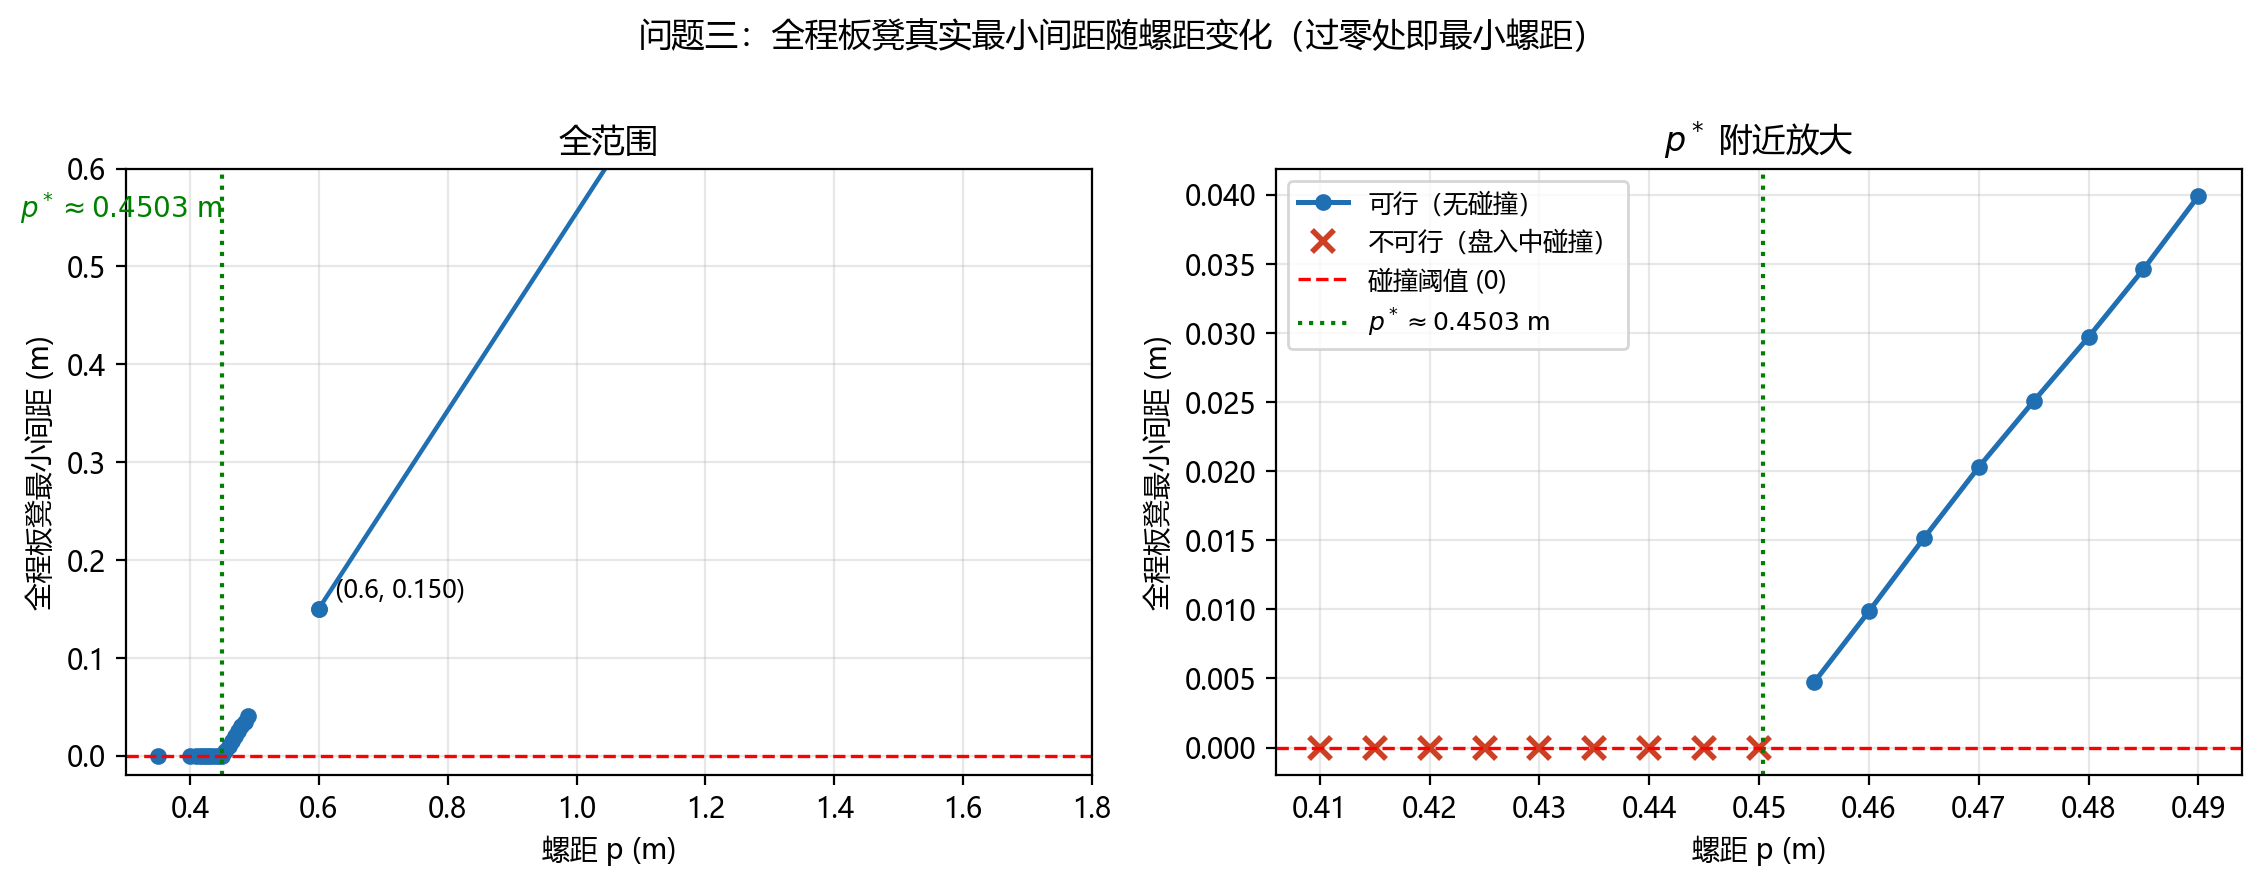
\includegraphics[width=0.68\textwidth]{figures/fig_问题三螺距搜索.png}
\caption{全程板凳真实最小间距随螺距变化（左：全范围；右：$p^{*}$ 附近放大，过零处即最小螺距）}
\label{fig:p3curve}
\end{figure}

\begin{figure}[H]
\centering
\begin{minipage}[t]{0.48\textwidth}
\centering
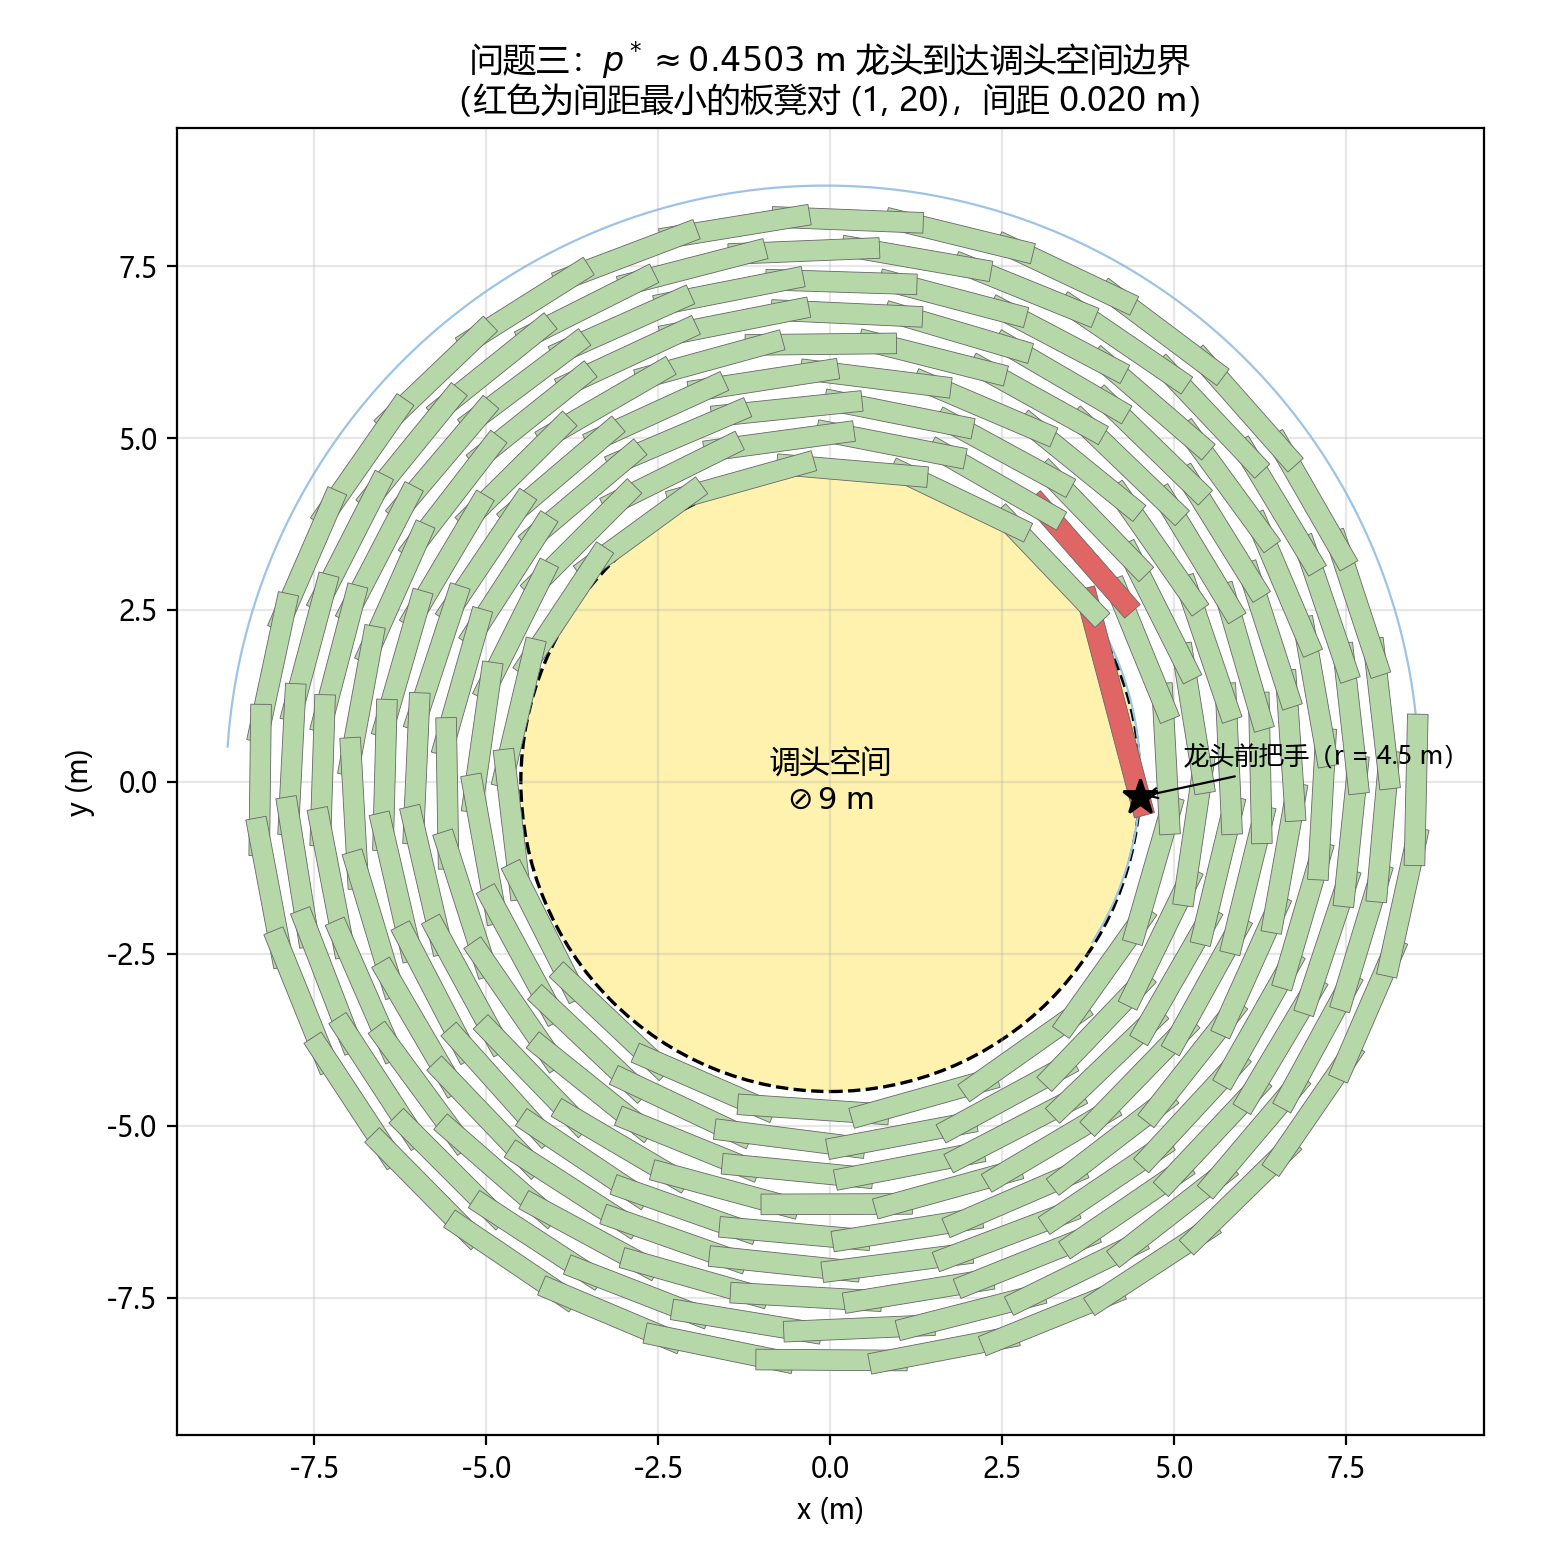
\includegraphics[width=0.97\textwidth]{figures/fig_问题三临界形态.png}
\caption{$p^{*}\approx0.4503\,\text{m}$ 时龙头恰好到达调头空间边界（$r=4.5\,\text{m}$）的整条龙形态（红色为间距最小的板凳对：龙头与第 20 节，间距 $0.020\,\text{m}$）}
\label{fig:p3crit}
\end{minipage}\hfill
\begin{minipage}[t]{0.48\textwidth}
\centering
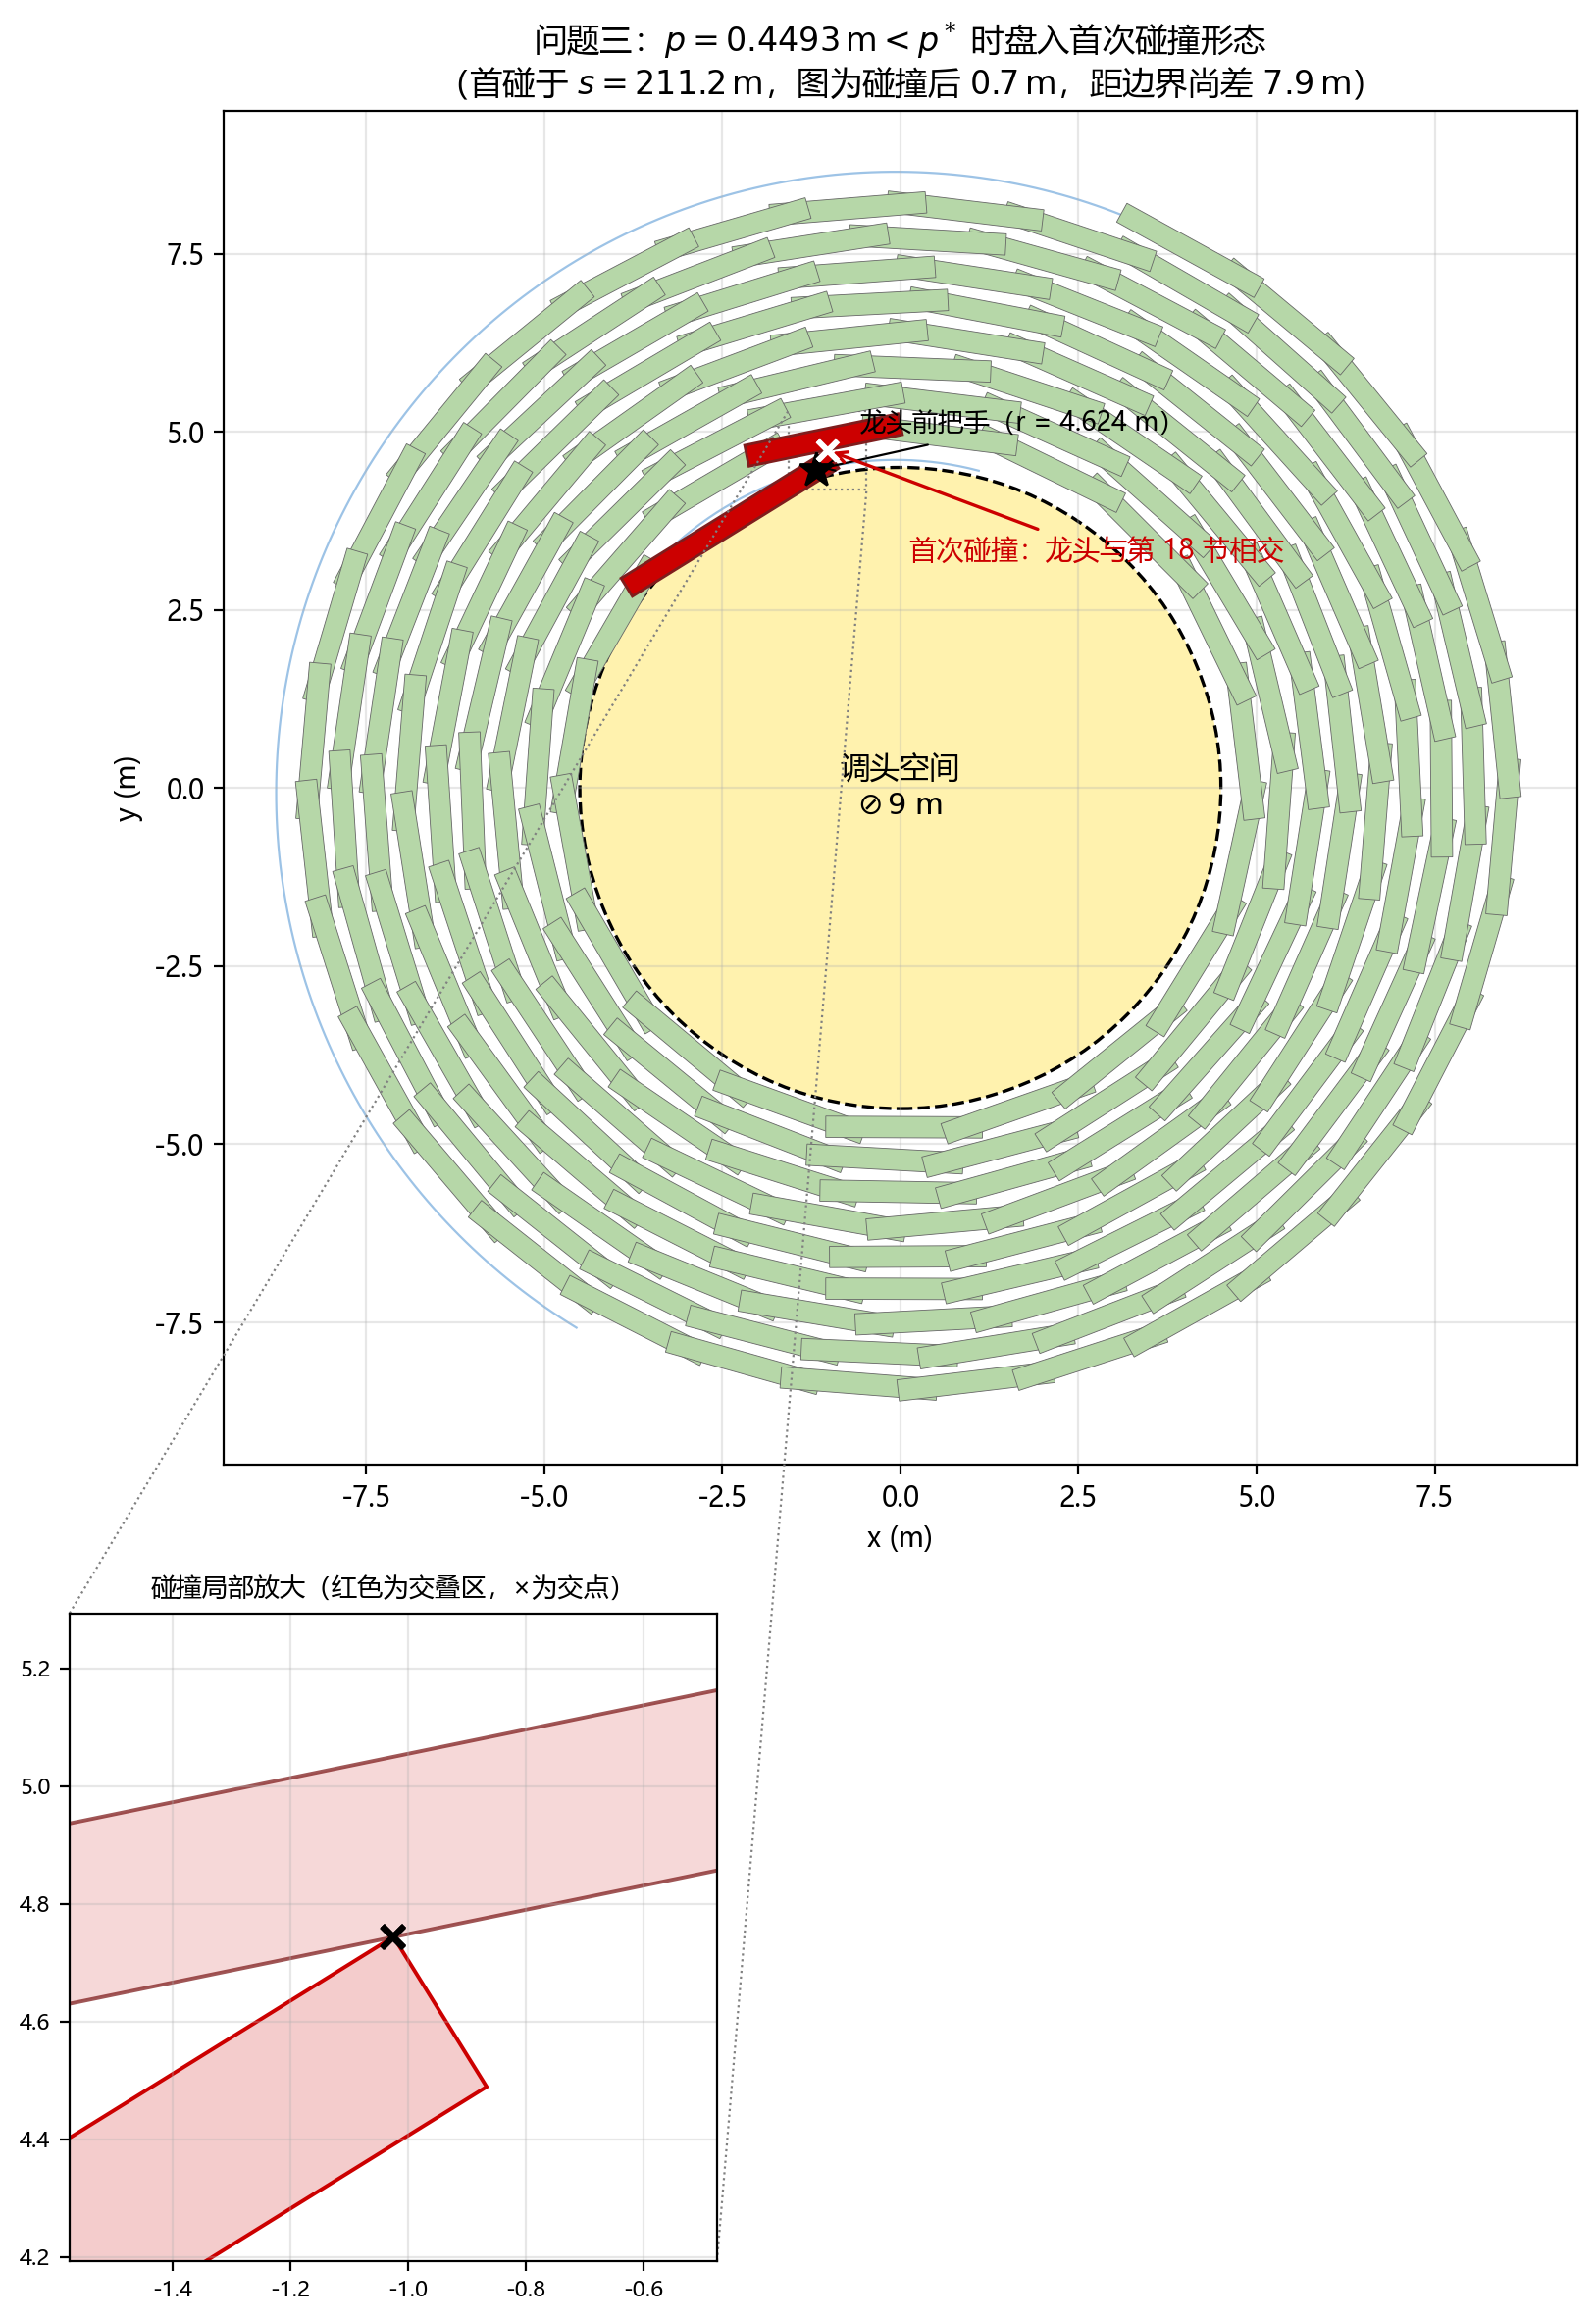
\includegraphics[width=0.97\textwidth]{figures/fig_问题三首碰形态.png}
\caption{$p=0.4493\,\text{m}<p^{*}$ 时盘入首次碰撞形态：龙头与相邻螺圈第 18 节板凳实体相交（红色，交点以 $\times$ 标注；左下插图为碰撞局部放大）。交叠呈切向滑过形成的瞬态细缝，首碰后约 $0.7\,\text{m}$ 交叠最深。}
\label{fig:p3collide}
\end{minipage}
\end{figure}

临界干涉结构在整个搜索过程中保持稳定：首碰板凳对恒为\textbf{龙头与相邻螺圈的龙身（第 18~24 节）}，空间上恰好相差约一圈；首碰位置随螺距减小而提前——$p=0.43\,\text{m}$ 时龙头在 $r=5.38\,\text{m}$ 处即碰，$p\to p^{*}$ 时首碰位置收敛到距边界约 $4.7\,\text{m}$ 处（龙头 $r\approx4.57\,\text{m}$），即最紧位置出现在龙头即将到达边界之前。图~\ref{fig:p3crit}（$p=p^{*}$ 时恰可达边界、最小间距 $0.020\,\text{m}$）与图~\ref{fig:p3collide}（$p<p^{*}$ 即发生实体相交，龙头距边界尚差约 $8.6\,\text{m}$ 弧长）互为对照，直观验证了 $p^{*}$ 的临界性：螺距再减 $10^{-3}\,\text{m}$ 量级，龙头便无法到达调头空间边界。

\subsubsection{结果合理性验证}
\begin{table}[H]
\centering
\caption{问题三结果合理性检验}
\label{tab:p3check}
\footnotesize
\begin{tabular}{llc}
\toprule
检验项 & 结果 & 判定 \\
\midrule
把手链几何精度（牛顿 vs Brent 逆推） & 最大极角差 $<2\times10^{-13}\,\text{rad}$ & $\checkmark$ 机器精度 \\
SAT 判定 vs Shapely 精确几何 & 无碰/相碰三构型逐一一致（相碰距离 $3\times10^{-17}\,\text{m}$） & $\checkmark$ \\
端点单调性 & $p=0.30$ 初始即碰；$p=1.70$ 全程无碰 & $\checkmark$ \\
二分一致性 & 14 次迭代无一违背单调结构 & $\checkmark$ \\
采样精度 & 临界区间隙—弧长斜率 $\sim10^{-3}\,\text{m/m}$，$ds=0.1\,\text{m}$ 采样影响 $\sim10^{-4}\,\text{m}$ & $\checkmark$ \\
物理标度 & $p^{*}\approx0.45\,\text{m}=$ 板宽 $0.30\,\text{m}$ + 约 $0.15\,\text{m}$ 弦/角点效应 & $\checkmark$ \\
速度无关性 & 构型序列仅由龙头弧长决定，$p^{*}$ 为纯几何量 & $\checkmark$ \\
\bottomrule
\end{tabular}
\end{table}

综上，最小螺距 $p^{*}\approx0.4503\,\text{m}$：以该螺距盘绕，龙头前把手可沿螺线无碰撞地到达直径 $9\,\text{m}$ 调头空间的边界，盘入总弧长约 $221\,\text{m}$（$221\,\text{s}$）、盘绕 6 圈；临界约束由龙头与相邻圈龙身的实体干涉给出，且入口处螺线与调头圆几乎曲率连续（$\rho=4.4994\,\text{m}$），为问题四在该调头空间内设计 S 形调头曲线、问题五分析调头段速度约束提供了几何基础。

\section{问题四模型的建立和求解}

\subsection{模型建立}

\subsubsection{调头场景设定与切点位置}
问题四中盘入螺线的螺距为 $p=1.7\,\text{m}$，即 $b=p/2\pi=0.270563\,\text{m}$；盘出螺线是盘入螺线关于螺线中心的\textbf{中心对称像} $\{-P(\theta)\}$。舞龙队沿盘入螺线顺时针盘入（$\theta$ 减小），到达调头空间边界后进入 S 形调头段，再逆时针盘出（$\theta$ 增大）。由问题三的设定，龙头前把手盘入至边界圆 $r=4.5\,\text{m}$ 处开始调头，故入口切点为盘入螺线与边界圆的交点
\begin{equation}
E=P(\theta_A),\qquad \theta_A=\frac{4.5}{b}=\frac{9\pi}{1.7}=16.631961\ \text{rad},
\end{equation}
行进方向沿螺线切向 $\mathbf{t}_E=-P'(\theta_A)/\|P'(\theta_A)\|$；出口切点为盘出螺线与边界圆的交点，由中心对称性 $F=-E$。注意到盘入（$\theta$ 减小）与盘出（$\theta$ 增大）在 $E$、$F$ 处的切向均为 $-P'(\theta_A)$ 方向，即 $\mathbf{t}_F=\mathbf{t}_E$——调头的实质是把整条龙横向平移约 $9\,\text{m}$，而非反向掉头，这一几何事实决定了 S 形曲线的结构。

\subsubsection{S 形曲线的相切几何}
S 形曲线由两段相切圆弧构成，要求 $R_1=2R_2$ 且与盘入、盘出螺线均相切。取弧 1 右转、弧 2 左转（曲率符号相反），则圆心由切点与左法向量 $\mathbf{n}=\mathrm{rot}_{90^\circ}(\mathbf{t}_E)$ 唯一确定：
\begin{equation}
O_1=E-R_1\mathbf{n},\qquad O_2=F+R_2\mathbf{n},
\end{equation}
两圆外切条件 $\|O_1-O_2\|=R_1+R_2$ 给出
\begin{equation}
\bigl\|\Delta+(R_1+R_2)\mathbf{n}\bigr\|=R_1+R_2,\qquad \Delta=F-E,
\end{equation}
解得半径之和为几何不变量
\begin{equation}
\boxed{\ S^*=R_1+R_2=-\frac{\|\Delta\|^2}{2\,\Delta\cdot\mathbf{n}}\ },
\end{equation}
代入数值 $\|\Delta\|=9\,\text{m}$、$\Delta\cdot\mathbf{n}=-8.9836\,\text{m}$，得 $S^*=4.508127\,\text{m}$，故
\begin{equation}
R_1=\tfrac{2}{3}S^*=3.005418\ \text{m},\qquad R_2=\tfrac{1}{3}S^*=1.502709\ \text{m}.
\end{equation}
弧间切点 $T$ 在连心线 $O_1O_2$ 上，$T=O_1+R_1\,\dfrac{O_2-O_1}{\|O_2-O_1\|}$。由位移 $\Delta$ 沿行进方向与横向的投影
\begin{equation}
\Delta\cdot\mathbf{t}_E = S\sin\gamma,\qquad \bigl|\Delta\cdot\mathbf{n}\bigr|=S(1-\cos\gamma),
\end{equation}
可得单段圆弧的扫角（两弧相等，合航向变化为零）
\begin{equation}
\tan\frac{\gamma}{2}=\frac{1-\cos\gamma}{\sin\gamma}=\frac{|\Delta\cdot\mathbf{n}|}{\Delta\cdot\mathbf{t}_E}
\quad\Longrightarrow\quad \gamma=3.021487\ \text{rad}=173.1184^\circ,
\end{equation}
调头曲线总长
\begin{equation}
L_0=R_1\gamma+R_2\gamma=S^*\gamma=13.621245\ \text{m}.
\end{equation}
数值验证（密采样弧上各点）表明该曲线最大极径恰为 $4.500000\,\text{m}$，即两端点触及边界圆、全程位于调头空间内。S 形调头曲线几何示意如图~\ref{fig:q4schem} 所示。

\begin{figure}[H]
\centering
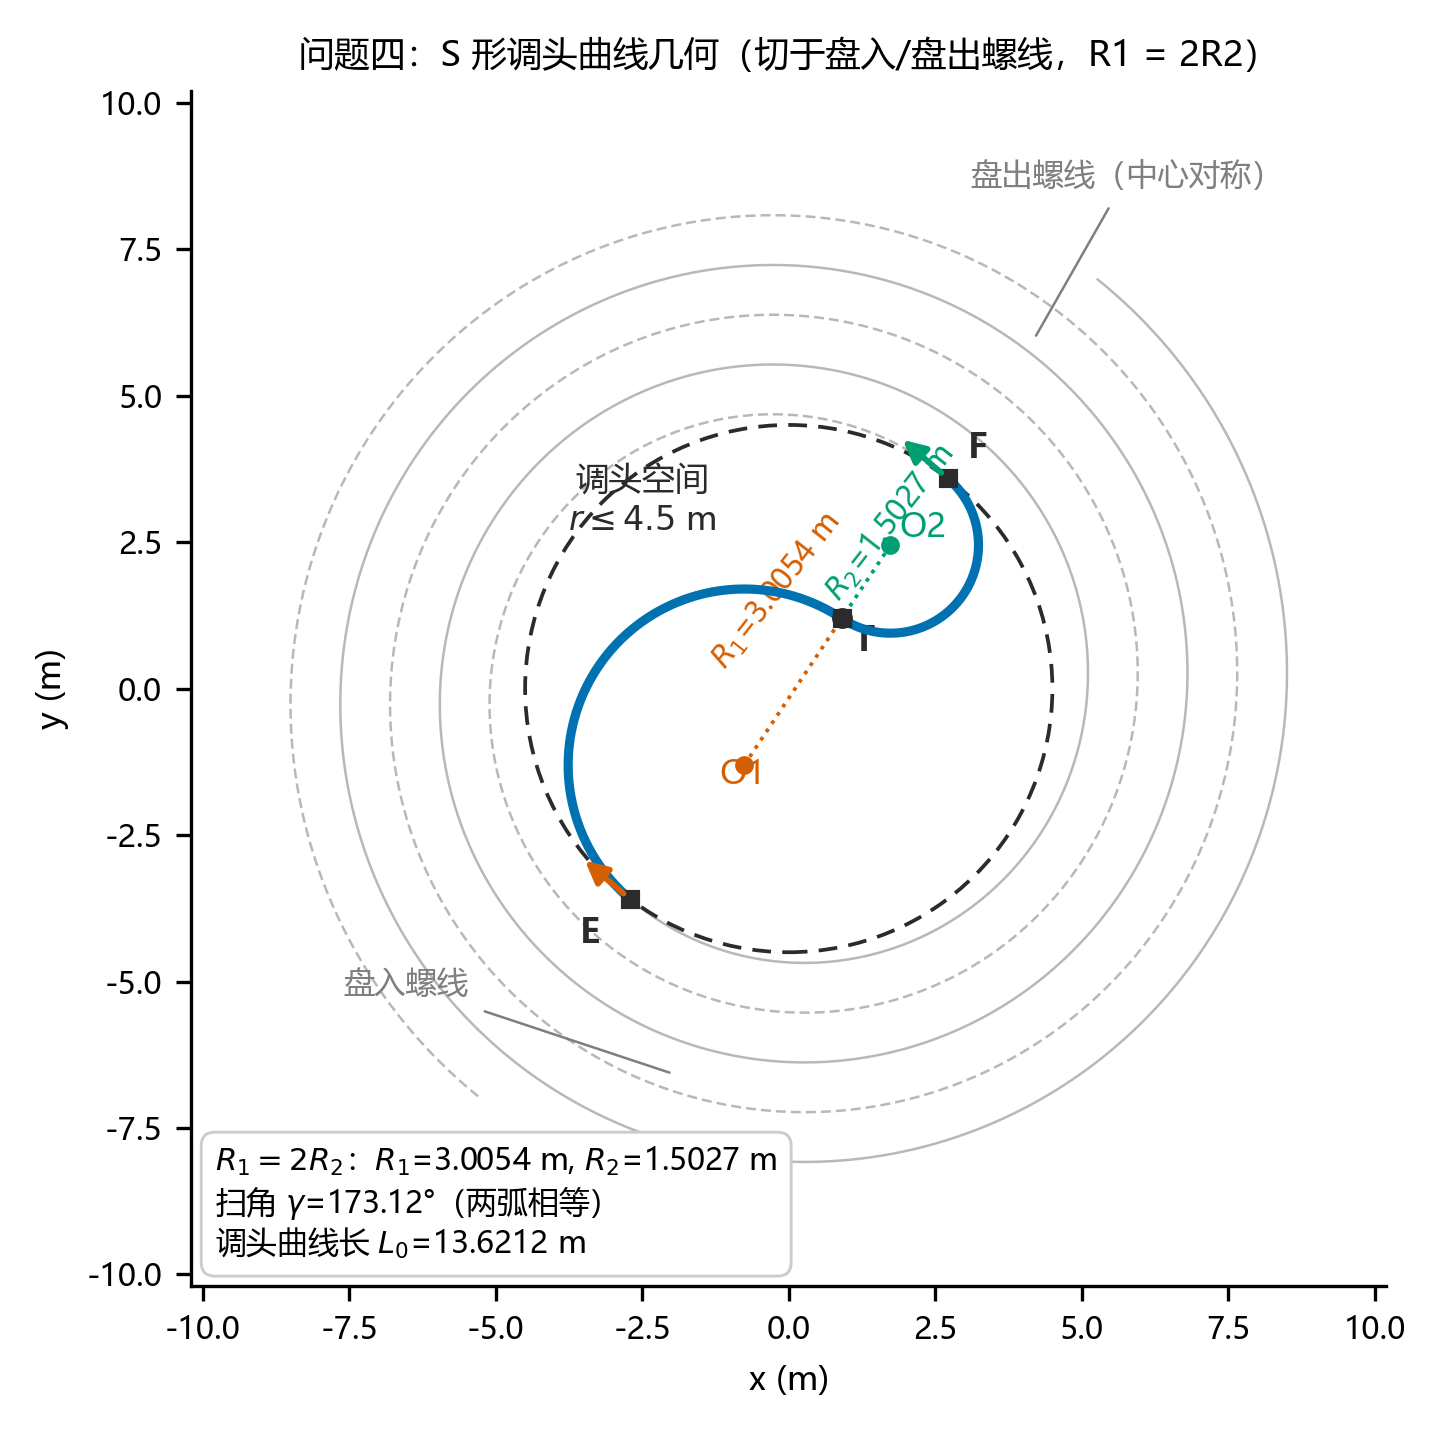
\includegraphics[width=0.51\textwidth]{figures/fig_问题四S形调头示意.png}
\caption{问题四 S 形调头曲线几何示意：实线为盘入螺线、虚线为中心对称的盘出螺线、蓝色为 S 形调头曲线；$E$、$F$ 为与两螺线的切点，$T$ 为弧间切点，$O_1$、$O_2$ 为两弧圆心，箭头为行进方向}
\label{fig:q4schem}
\end{figure}

\subsubsection{复合轨迹曲线与逆推法的推广}
定义龙头前把手的轨迹 $C$，以弧长 $u$ 为参数（$u=0$ 在入口切点 $E$，沿行进方向递增）：
\begin{equation}
C(u)=
\begin{cases}
P\bigl(\theta(s)\bigr), & u<0\ \ (\text{盘入螺线},\ \theta\ \text{递减}),\\[2pt]
O_1+R_1\bigl(\cos\phi_1(u),\,\sin\phi_1(u)\bigr), & 0\le u\le R_1\gamma\ \ (\text{弧 1},\ \text{顺时针}),\\[2pt]
O_2+R_2\bigl(\cos\phi_2(u),\,\sin\phi_2(u)\bigr), & R_1\gamma<u\le L_0\ \ (\text{弧 2},\ \text{逆时针}),\\[2pt]
-P\bigl(\theta(s)\bigr), & u>L_0\ \ (\text{盘出螺线},\ \theta\ \text{递增}),
\end{cases}
\end{equation}
其中 $s(\theta)=\tfrac{b}{2}\bigl[\theta\sqrt{1+\theta^2}+\operatorname{arsinh}\theta\bigr]$ 为螺线弧长（半解析式），$\theta(s)$ 由牛顿迭代反解（双精度收敛）。四段在接缝 $u=0$、$R_1\gamma$、$L_0$ 处切向连续（$C^1$），数值校验通过。

将问题一“各把手中心均位于螺线上”的逆推法\textbf{推广为“各把手均位于复合轨迹 $C$ 上”}：相邻把手沿 $C$ 的弦长恒为孔距，
\begin{equation}
\bigl\|C(u_{i+1})-C(u_i)\bigr\|=D_i,\qquad D_1=2.86\ \text{m},\quad D_{2\sim223}=1.65\ \text{m},
\end{equation}
龙头位置 $u_1=t$（恒速 $1\,\text{m/s}$，$t=0$ 开始调头），对每个 $i$ 在 $u_i$ 后方区间 $[\,u_i-2.6D_i,\ u_i-0.4D_i\,]$ 内用 Brent 法解弦长方程取唯一根（相邻把手弦长远小于局部单调解，根唯一）。速度仍沿用刚体铰接链速度分解递推：
\begin{equation}
v_{i+1}=v_i\,\frac{\boldsymbol{\tau}(u_i)\cdot\mathbf{e}_i}{\boldsymbol{\tau}(u_{i+1})\cdot\mathbf{e}_i},\qquad \mathbf{e}_i=\frac{C(u_{i+1})-C(u_i)}{\|C(u_{i+1})-C(u_i)\|},
\end{equation}
其中 $\boldsymbol{\tau}(u)$ 为 $C$ 的单位切向（分段解析），$v_1\equiv1$；与二阶中心差分交叉验证偏差 $<10^{-6}\,\text{m/s}$。

\subsubsection{第二问的优化模型}
“能否调整圆弧，仍是各部分相切，使调头曲线变短”按结构调整自由度分为两个层次。

\textbf{(a) 仅调整半径比例（两弧族）：长度不变性定理。}对任意分配 $R_1+R_2=S$，由 $O_1=E-R_1\mathbf{n}$、$O_2=F+R_2\mathbf{n}$ 得 $O_1-O_2=-\Delta-S\mathbf{n}$，故外切条件 $\|O_1-O_2\|=S$ \textbf{与分配无关地唯一确定} $S=S^*$；又切点 $T$ 虽随分配移动，但由弦长几何可知两弧扫角恒为
\begin{equation}
\gamma=2\arcsin\frac{\|\mathbf{n}+\hat{m}\|}{2}=\text{常量}\quad(\hat{m}=\tfrac{O_2-O_1}{\|O_2-O_1\|}),
\end{equation}
因此调头曲线长度
\begin{equation}
\boxed{\ L=R_1\gamma+R_2\gamma=S^{*}\gamma=13.621245\ \text{m}\ }
\end{equation}
\textbf{在切点固定的两弧族内为不变量}——无论 $R_1:R_2$ 取何比例，调头曲线长度均不变。故仅调整半径比例不能变短。

\textbf{(b) 调整曲线结构（弧–线–弧）：可显著缩短。}允许在弧 1 与弧 2 之间加入公切线段（长 $\ell\ge0$，仍与两螺线及彼此相切）。以弧 1 半径 $R_1$ 与扫角 $\alpha$ 为自由参数，其余量由相切条件解析确定：
\begin{equation}
T_1=E+R_1\sin\alpha\,\mathbf{t}_E-R_1(1-\cos\alpha)\,\mathbf{n},\qquad \mathbf{m}=\mathrm{rot}(\mathbf{t}_E,-\alpha),
\end{equation}
\begin{equation}
R_2=\frac{(F-T_1)\cdot\mathbf{n}_m}{1-\cos\alpha},\qquad \ell=(F-T_1)\cdot\mathbf{m}-R_2\sin\alpha\ \ (\ge0),
\end{equation}
$\mathbf{n}_m=\mathrm{rot}_{90^\circ}(\mathbf{m})$。目标与约束为
\begin{equation}
\min_{R_1,\alpha}\ L=(R_1+R_2)\alpha+\ell
\quad\text{s.t.}\quad \ell\ge0,\ R_1,R_2\ge\tfrac{D_{\text{body}}}{2}=0.825\ \text{m},\ r\le4.5\ \text{m},
\end{equation}
其中半径下界 $D_{\text{body}}/2$ 来自\textbf{可跟随性}：孔距 $1.65\,\text{m}$ 的板凳弦须能落在圆弧上，弧半径不得小于弦长之半，否则相邻把手无法同时位于同一圆弧上、链条几何失效。采用网格粗搜 $+$ Nelder–Mead 局部精修求解。

\subsection{模型求解}

\subsubsection{全龙仿真与关键时刻结果}
对 $t\in[-100,100]$ 每秒递推全部 224 个把手位置与速度（保留 6 位小数）并存入 \texttt{result4.xlsx}。论文要求的 $-100,-50,0,50,100\,\text{s}$ 五个关键时刻指定把手的位置与速度如表~\ref{tab:q4pos}、表~\ref{tab:q4vel} 所示。

\begin{table}[H]
\centering
\caption{问题四各关键时刻指定把手的位置（单位：m）}
\label{tab:q4pos}
\footnotesize\setlength{\tabcolsep}{3.6pt}
\renewcommand{\arraystretch}{1.15}
\begin{tabular}{lrrrrr}
\toprule
 & $-100$ s & $-50$ s & $0$ s & $50$ s & $100$ s \\
\midrule
龙头 $x$ & 7.778034 & 6.608301 & $-2.711856$ & 1.332696 & $-3.157229$ \\
龙头 $y$ & 3.717164 & 1.898865 & $-3.591078$ & 6.175324 & 7.548511 \\
第 1 节龙身 $x$ & 6.209273 & 5.366911 & $-0.063534$ & 3.862265 & $-0.346890$ \\
第 1 节龙身 $y$ & 6.108521 & 4.475403 & $-4.670888$ & 4.840828 & 8.079166 \\
第 51 节龙身 $x$ & $-10.608038$ & $-3.629945$ & 2.459962 & $-1.671385$ & 2.095033 \\
第 51 节龙身 $y$ & 2.831491 & $-8.963800$ & $-7.778145$ & $-6.076713$ & 4.033787 \\
第 101 节龙身 $x$ & $-11.922761$ & 10.125787 & 3.008493 & $-7.591816$ & $-7.288774$ \\
第 101 节龙身 $y$ & $-4.802378$ & $-5.972247$ & 10.108539 & 5.175487 & 2.063875 \\
第 151 节龙身 $x$ & $-14.351032$ & 12.974784 & $-7.002789$ & $-4.605165$ & 9.462513 \\
第 151 节龙身 $y$ & $-1.980993$ & $-3.810357$ & 10.337482 & $-10.386988$ & $-3.540357$ \\
第 201 节龙身 $x$ & $-11.952942$ & 10.522509 & $-6.872842$ & 0.336952 & 8.524374 \\
第 201 节龙身 $y$ & 10.566998 & $-10.807425$ & 12.382609 & $-13.177610$ & 8.606933 \\
龙尾（后）$x$ & $-1.011059$ & 0.189809 & $-1.933627$ & 5.859094 & $-10.980157$ \\
龙尾（后）$y$ & $-16.527573$ & 15.720588 & $-14.713128$ & 12.612894 & $-6.770006$ \\
\bottomrule
\end{tabular}
\end{table}

\begin{table}[H]
\centering
\caption{问题四各关键时刻指定把手的速度（单位：m/s）}
\label{tab:q4vel}
\footnotesize\setlength{\tabcolsep}{3.6pt}
\renewcommand{\arraystretch}{1.15}
\begin{tabular}{lrrrrr}
\toprule
 & $-100$ s & $-50$ s & $0$ s & $50$ s & $100$ s \\
\midrule
龙头 & 1.000000 & 1.000000 & 1.000000 & 1.000000 & 1.000000 \\
第 1 节龙身 & 0.999904 & 0.999762 & 0.998687 & 1.000363 & 1.000124 \\
第 51 节龙身 & 0.999346 & 0.998642 & 0.995134 & 0.949935 & 1.003966 \\
第 101 节龙身 & 0.999091 & 0.998248 & 0.994448 & 0.948482 & 1.096263 \\
第 151 节龙身 & 0.998944 & 0.998047 & 0.994156 & 0.948038 & 1.095306 \\
第 201 节龙身 & 0.998849 & 0.997925 & 0.993994 & 0.947823 & 1.094933 \\
龙尾（后） & 0.998817 & 0.997885 & 0.993944 & 0.947760 & 1.094833 \\
\bottomrule
\end{tabular}
\end{table}

几何与物理校验：把手链弦长残差 $\max\bigl|\|P_{i+1}-P_i\|-D_i\bigr|=1.3\times10^{-13}\,\text{m}$；复合轨迹在 $u=0,\ R_1\gamma,\ L_0$ 三处切向连续（偏差 $<10^{-5}$）；速度递推与中心差分交叉验证偏差 $<10^{-6}\,\text{m/s}$。全龙形态如图~\ref{fig:q4shots} 所示；速度场的完整特征为：整数秒采样内最大把手速度 $1.4222\,\text{m/s}$（$t=14\,\text{s}$，第 2 把手），连续峰值出现于龙头穿越弧 2 曲率切换区前后——这正是问题五提速瓶颈之所在。

\begin{figure}[H]
\centering
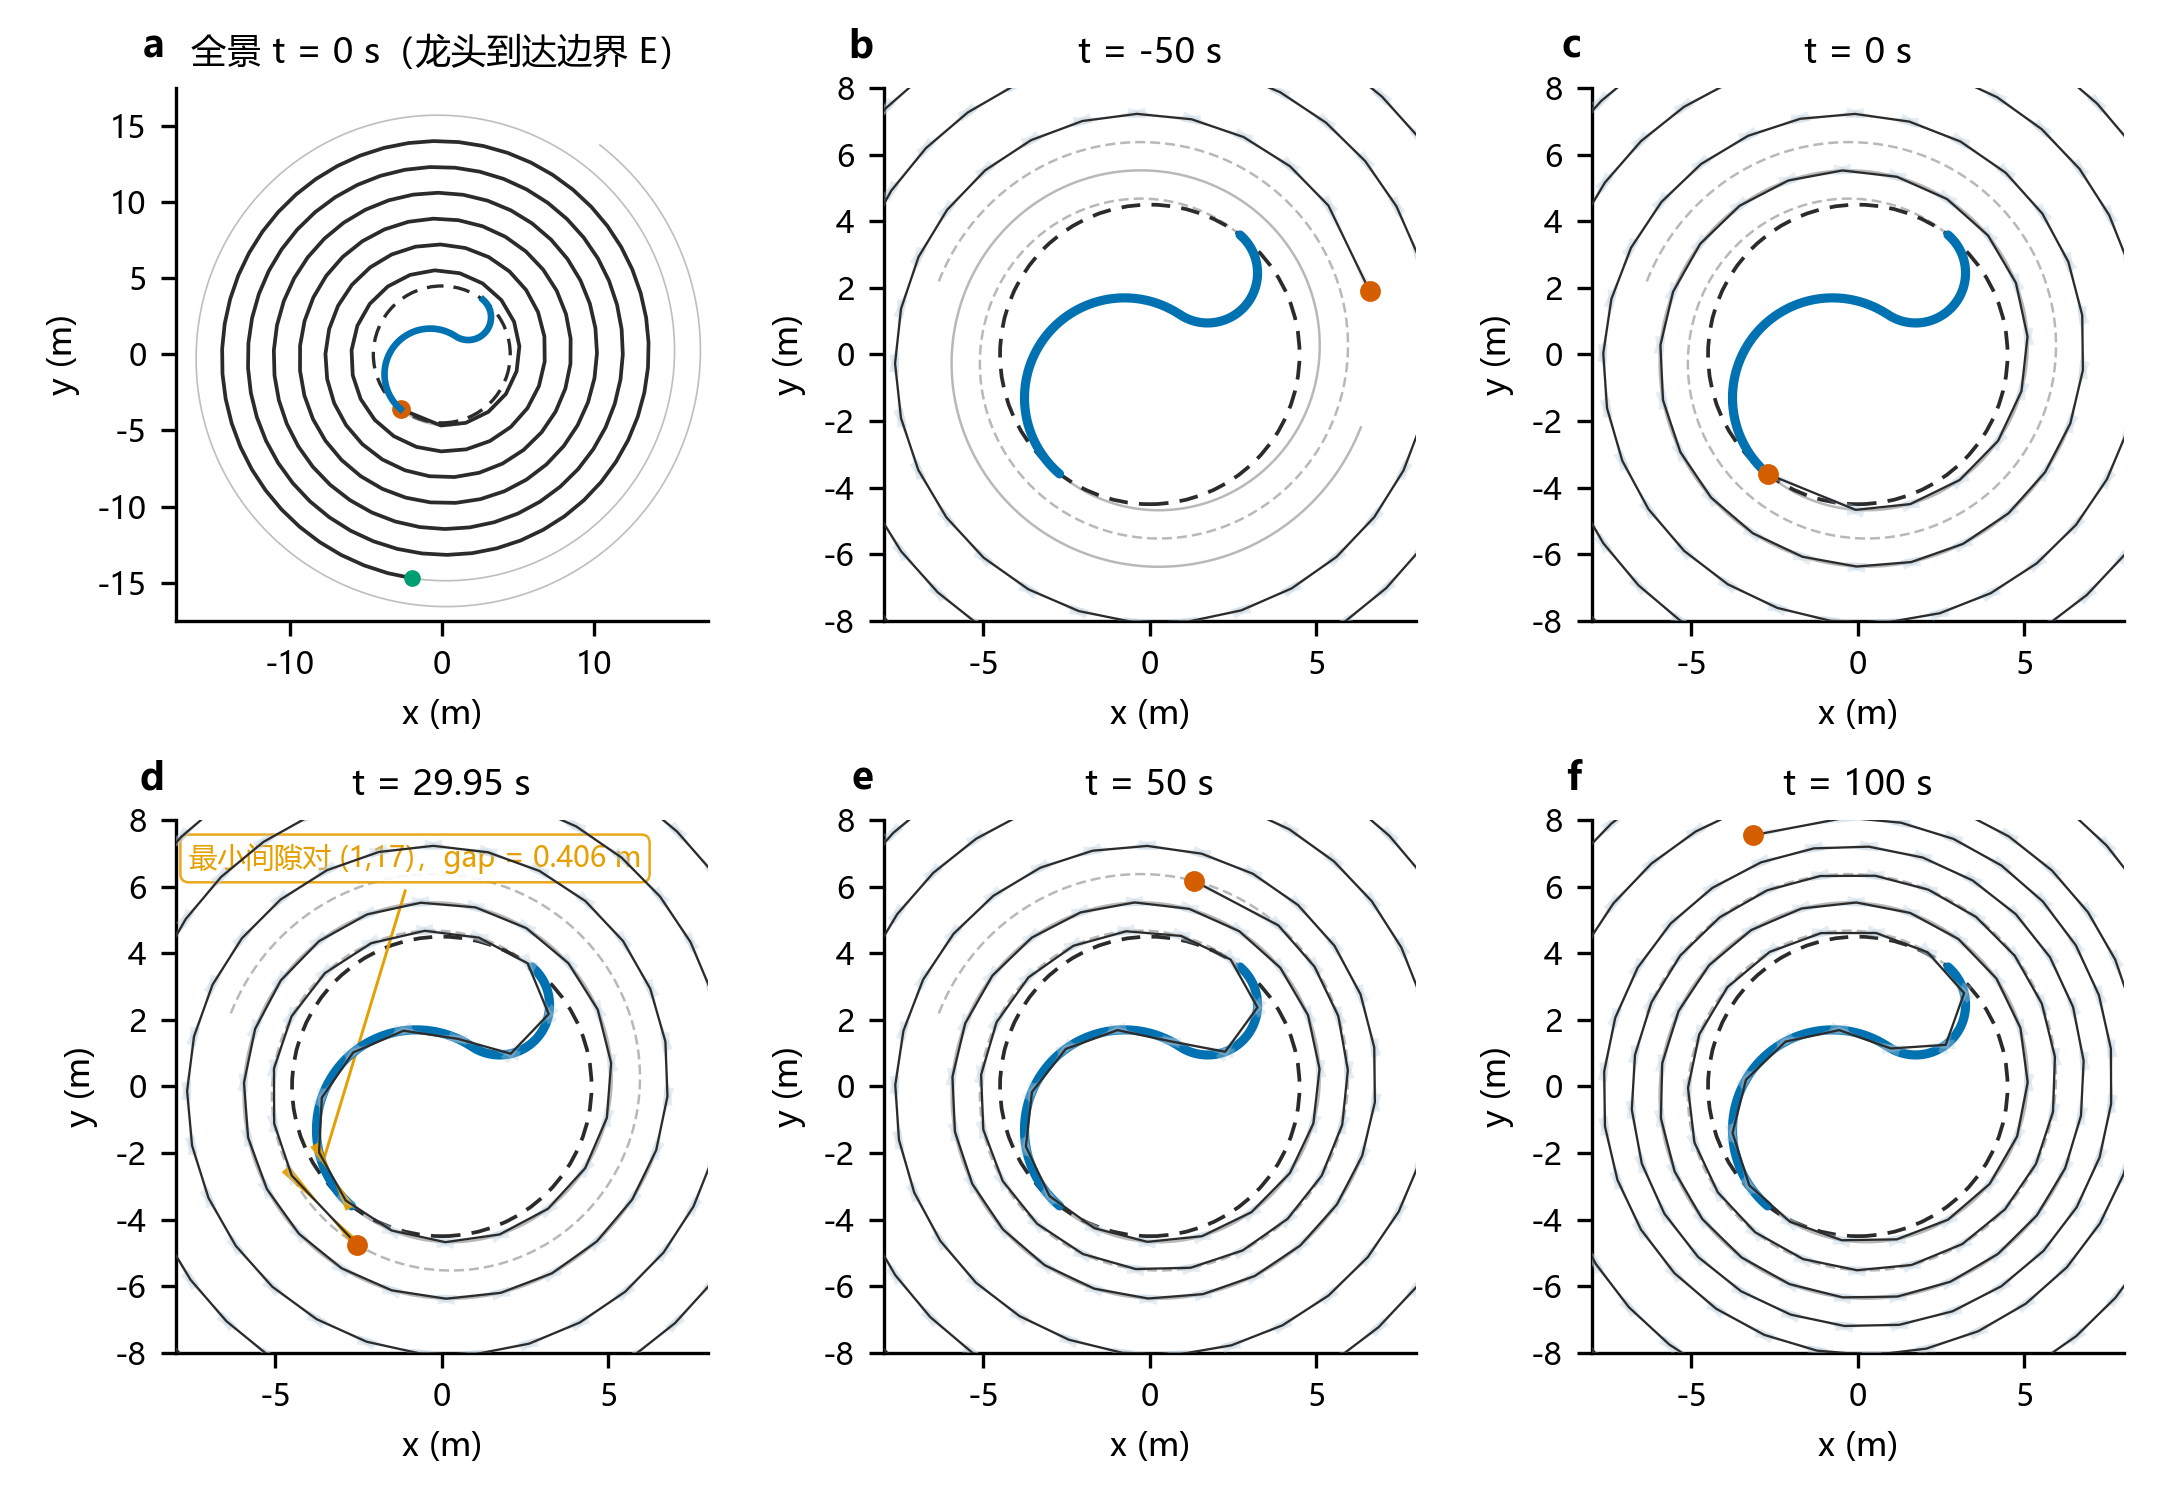
\includegraphics[width=0.61\textwidth]{figures/fig_问题四全龙构型.png}
\caption{问题四全龙构型：（a）$t=0$ 全景（龙头到达边界 $E$）；（b--f）$t=-50,0,29.95,50,100$ s 调头区放大快照，红/绿为龙头与龙尾，橙色高亮为最小间隙对 $(1,17)$}
\label{fig:q4shots}
\end{figure}

速度特征与物理机理：$t\le0$ 全龙在盘入螺线上，各把手速度略低于并趋近 $1\,\text{m/s}$；$t\approx50\,\text{s}$ 龙身中段穿越 S 弯时速度压降至 $\approx0.948\,\text{m/s}$（S 弯总弧长 $13.62\,\text{m}$ 大于其弦向跨度，链条在弯内“拥挤”减速）；$t\approx100\,\text{s}$ 龙身进入盘出螺线内侧圈时回升至 $\approx1.095\,\text{m/s}$（内圈曲率大、后把手被迫加速）。速度峰值位于龙头穿越弧 1 至弧 2 的曲率反向切换点 $T$ 前后：整数秒采样最大 $1.422195\,\text{m/s}$（$t=14\,\text{s}$，第 2 把手），$0.1\,\text{s}$ 加密采样连续峰值 $\approx1.604\,\text{m/s}$（$t\approx14.5\,\text{s}$，第 5 把手附近）。

\subsubsection{碰撞可行性验证}
沿用问题二的旋转矩形干涉判据（AABB 宽相预筛 + SAT/顶点包容精相，以 Shapely 精确欧氏距离复核），对 $t\in[-100,100]$ 全程扫描（$|t|\le25$ 内加密至 $\Delta t=0.25\,\text{s}$，最小值邻域加密至 $0.05\,\text{s}$）：基线调头曲线全程最小板凳间隙为 $0.406088\,\text{m}$（板凳对 $(1,17)$，$t=29.95\,\text{s}$），全程无碰撞。

\subsubsection{可否变短：(a) 两弧族内不变性验证}
固定切点 $E,F$，对比例 $k=R_1/R_2$ 求解外切配置并数值积分弧长，结果见表~\ref{tab:q4invar}。

\begin{table}[H]
\centering
\caption{两弧族内调头曲线长度不变性验证（切点固定于 $E,F$）}
\label{tab:q4invar}
\footnotesize\setlength{\tabcolsep}{5pt}
\renewcommand{\arraystretch}{1.12}
\begin{tabular}{crrrcrr}
\toprule
$k=R_1/R_2$ & $R_1$ (m) & $R_2$ (m) & $R_1+R_2$ (m) & $\gamma$ (rad) & $L$ (m) & 在调头空间内 \\
\midrule
0.25 & 0.901625 & 3.606501 & 4.508127 & 3.021487 & \textbf{13.621245} & $\checkmark$ \\
2.00（题目） & 3.005418 & 1.502709 & 4.508127 & 3.021487 & \textbf{13.621245} & $\checkmark$ \\
5.00 & 3.756772 & 0.751354 & 4.508127 & 3.021487 & \textbf{13.621245} & $\checkmark$ \\
\bottomrule
\end{tabular}
\end{table}

全部六种受测比例（$k\in\{0.25,0.5,1,2,3,5\}$）下 $R_1+R_2$、扫角 $\gamma$、长度 $L$ 逐一相等（小数点后 6 位一致），与不变性定理完全吻合。\textbf{因此：仅调整两弧的半径比例，调头曲线长度不变，不能变短。}

\subsubsection{可否变短：(b) 弧–线–弧结构优化}
在 $(R_1,\alpha)$ 平面网格粗搜（$R_1\in[0.825,3.2]$ 共 30 点、$\alpha\in[0.3,3.0]$ 共 80 点）$+$ Nelder–Mead 局部精修，约束为 $\ell\ge0$、$R_1,R_2\ge D_{\text{body}}/2$、曲线位于调头空间内。$R_1$ 敏感性见表~\ref{tab:q4sens}。

\begin{table}[H]
\centering
\caption{弧–线–弧结构 $R_1$ 敏感性（每档取该 $R_1$ 下最优 $\alpha$）}
\label{tab:q4sens}
\footnotesize\setlength{\tabcolsep}{5pt}
\renewcommand{\arraystretch}{1.12}
\begin{tabular}{crrrr}
\toprule
$R_1$ (m) & $\alpha$ ($^\circ$) & $R_2$ (m) & $\ell$ (m) & $L^{*}$ (m) \\
\midrule
\textbf{0.825（下界）} & \textbf{99.43} & \textbf{0.897827} & \textbf{7.074123} & \textbf{10.064165} \\
1.00 & 101.94 & 0.9762 & 6.7447 & 10.26029 \\
1.20 & 103.49 & 0.9241 & 6.5449 & 10.38103 \\
1.50 & 107.36 & 0.9620 & 6.0633 & 10.67679 \\
2.00 & 113.60 & 0.9208 & 5.3405 & 11.13067 \\
2.50 & 122.13 & 0.9180 & 4.4258 & 11.71171 \\
\bottomrule
\end{tabular}
\end{table}

$L^{*}$ 随 $R_1$ 单调增大，最优解落在可跟随性下界 $R_1=D_{\text{body}}/2$ 处；若继续减小半径，则相邻把手无法同时位于同一圆弧上，链条几何失效。最优解几何参数如表~\ref{tab:q4opt} 所示。

\begin{table}[H]
\centering
\caption{弧–线–弧最优解几何参数}
\label{tab:q4opt}
\footnotesize
\begin{tabular}{lc}
\toprule
量 & 数值 \\
\midrule
弧 1 半径 $R_1$ / 弧 2 半径 $R_2$ & $0.825100$ / $0.897827$ m \\
两弧扫角 $\alpha$ & $1.735443$ rad（$99.4336^\circ$） \\
公切线段长 $\ell$ & $7.074123$ m \\
弧 1 圆心 $O_1$ / 弧 2 圆心 $O_2$ & $(-2.176001,\,-2.963663)$ / $(2.128768,\,2.908360)$ \\
弧–线切点 $T_1$ / 线–弧切点 $T_2$ & $(-2.707102,\,-2.332219)$ / $(2.706683,\,2.221258)$ \\
\textbf{调头曲线长度 $L^{*}$} & \textbf{10.064165 m} \\
相对基线 $L_0=13.621245$ & 缩短 $3.557080$ m（$-26.11\%$） \\
曲线最大极径 & $4.500000$ m（仍在调头空间内） \\
\bottomrule
\end{tabular}
\end{table}

对最优弧–线–弧曲线重复全程碰撞扫描：最小板凳间隙为 $0.273425\,\text{m}$（$t=13.75\,\text{s}$），全程无碰撞。两弧族不变性与弧–线–弧优化曲线如图~\ref{fig:q4opt} 所示。

\begin{figure}[H]
\centering
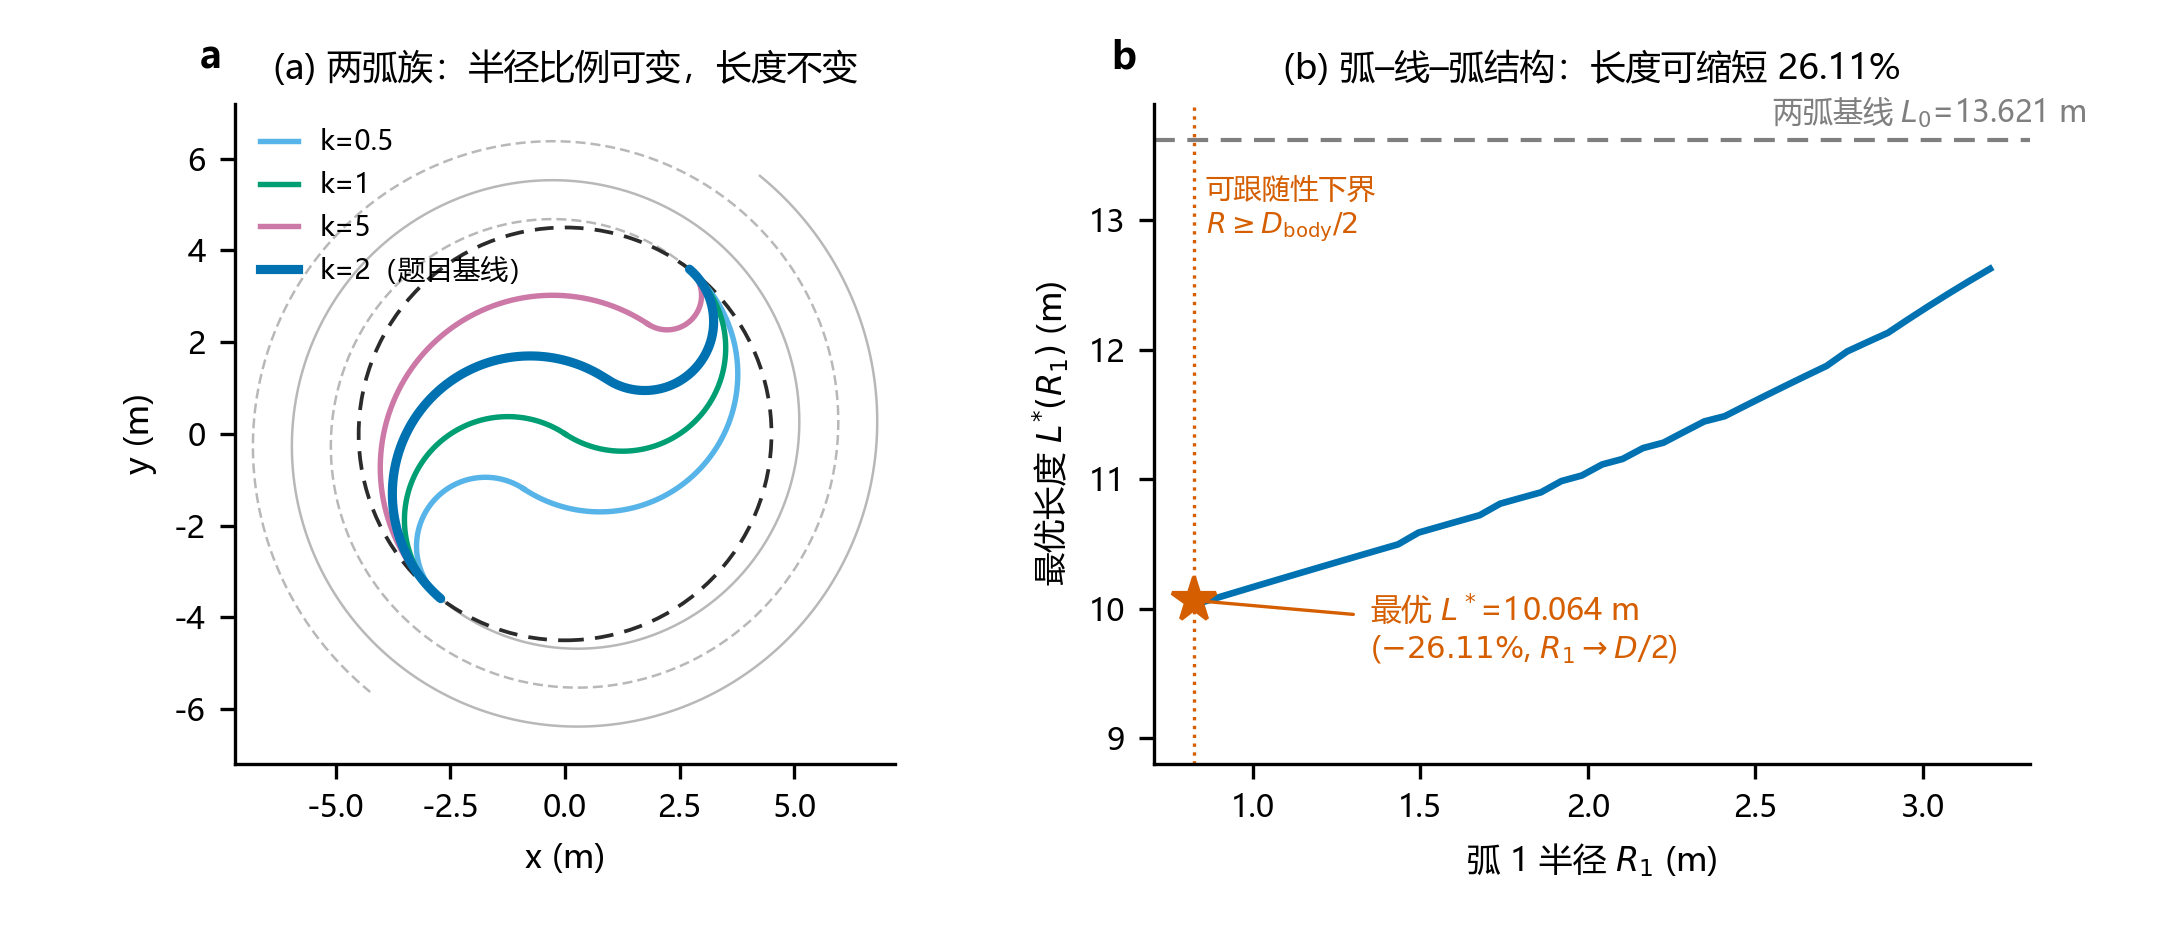
\includegraphics[width=0.61\textwidth]{figures/fig_问题四曲线族与优化.png}
\caption{问题四“能否变短”分析：（a）切点固定的两弧族，半径比例（$k=0.5,1,2,5$）可变但长度不变（均为 $13.621\,\text{m}$）；（b）弧–线–弧结构的最优长度 $L^{*}(R_1)$ 曲线，最短 $L^{*}=10.064\,\text{m}$（$-26.11\%$），虚线为两弧基线 $L_0$}
\label{fig:q4opt}
\end{figure}

\subsubsection{问题四小结}
综上：第一问求得 S 形调头曲线 $R_1=3.005418\,\text{m}$、$R_2=1.502709\,\text{m}$、扫角 $\gamma=173.1184^\circ$、总长 $L_0=13.621245\,\text{m}$（内切于直径 $9\,\text{m}$ 调头空间），并完成 $-100\sim100\,\text{s}$ 全龙 224 节点位置与速度递推；第二问结论为：(a) 仅调整两弧半径比例不能变短（不变性定理）；(b) 弧–线–弧结构可将调头曲线缩至 $L^{*}=10.064165\,\text{m}$（\textbf{缩短 26.11\%}），且全程位于调头空间内、全龙无碰撞。缩短的本质是用直线替代部分高曲率弧段；理论下界为横向位移量 $8.9836\,\text{m}$，受板凳可跟随性（$R\ge D_{\text{body}}/2$）约束，实际最优在 $R_1\to0.825\,\text{m}$ 处取得。

%% ========================================================
%% 问题五模型的建立与求解
%% ========================================================
\section{问题五模型的建立和求解}

\subsection{模型建立}

\subsubsection{齐次性约化：从“时间—把手”无穷族约束到一元全局最大化}
设龙头以恒定速度 $v$ 沿问题四的复合轨迹 $C$（弧长参数 $u$）行进，龙头弧长位置 $u_1(t)=v\,t$（$t=0$ 为调头开始）。各把手位于 $C$ 上、相邻弦长恒为孔距，故全部把手位置由弦长方程组唯一确定，可写为 $u_i=U_i(u_1)$（$U_i$ 除接缝事件点外为光滑隐函数）。由链式法则，第 $i$ 把手速度
\begin{equation}
\bigl\|\dot{X}_i(t)\bigr\|=\bigl\|C'\!\bigl(U_i(u_1)\bigr)\bigr\|\cdot\bigl|U_i'(u_1)\bigr|\cdot v
= v\,\rho_i(u_1),
\label{eq:q5_homo}
\end{equation}
其中 $C'$ 为单位切向量，$\rho_i(u_1)=|U_i'(u_1)|$ 为\textbf{速度传递比}——它只依赖几何构型，与 $v$、$t$ 均无关（\textbf{齐次性引理}）。于是“任意时刻、任意把手速度 $\le 2\,\text{m/s}$”的二维无穷族约束等价于
\begin{equation}
v\,\max_{u_1,\,i}\rho_i(u_1)\le 2
\quad\Longleftrightarrow\quad
v\le v^{*}=\frac{2}{R_{\max}},\qquad
R_{\max}=\max_{u_1\in\mathbb{R},\,1\le i\le224}\rho_i(u_1).
\label{eq:q5_reduce}
\end{equation}
问题化为\textbf{一元全局最大化}：以 $v=1\,\text{m/s}$ 虚拟行进（复用问题四速度场），求速度比场的全局峰值。

\subsubsection{弦切角速度传递与同弧段恒速引理}
对弦长约束 $\|C(u_{i+1})-C(u_i)\|^2=D_i^2$ 关于 $u_1$ 求导，得速度传递的弦切角形式
\begin{equation}
\rho_{i+1}=\rho_i\,\frac{\cos\alpha_j}{\cos\beta_j}
=\rho_i\,\frac{\boldsymbol{\tau}(u_i)\cdot\mathbf{e}_i}{\boldsymbol{\tau}(u_{i+1})\cdot\mathbf{e}_i},
\qquad
\rho_i=\prod_{j<i}\frac{\cos\alpha_j}{\cos\beta_j},
\label{eq:q5_transfer}
\end{equation}
其中 $\mathbf{e}_i$ 为弦方向单位向量，$\alpha_j$、$\beta_j$ 为弦在前、后把手处的弦切角。$\rho_{i+1}>\rho_i\iff\beta_j>\alpha_j$，即弦与\textbf{后把手}切向更“横”——这发生在后把手一侧曲率更大时：曲率半径 $R$ 上的弦切角约 $\psi(D,R)=\arcsin\frac{D}{2R}$。本路径各段特征弦切角为：弧 2（$R_2=1.5027\,\text{m}$）$33.3^\circ$、弧 1（$R_1=3.0054\,\text{m}$）$16.0^\circ$、螺线缝邻域（$\rho_c=4.49\,\text{m}$）$10.6^\circ$——弧 2 曲率最大，峰值必出现在把手链穿越弧 2 及其两侧接缝（$T$、$F$）的窗口。

\noindent\textbf{引理（同弧段恒速）}\quad 若把手 $i,i+1$ 同在一段圆弧上，则同一圆上等弦的弦切角相等（$\alpha_j=\beta_j$），代入式~\eqref{eq:q5_transfer} 得 $\rho_{i+1}=\rho_i$。即速度比沿把手编号在每段圆弧内部为常值，放大只发生在接缝跨越处，且同弧段内各把手\textbf{并列}取得该值。

搜索域可截断为 $u_1\in[-70,410]$：链条总长 $369.2\,\text{m}$，当龙头远离 S 弯（$|u_1-$ 缝$|$ 充分大）时全部把手处于单一螺线段上，螺线曲率半径随 $\theta$ 单调增大，比场单调回落至 $1$；数值复核 $u_1\le-70$ 时 $\max_i\rho_i=1.000000$，$u_1\in[395,460]$ 时 $\max_i\rho_i\le1.0038$ 且单调递减，均远小于候选峰值。

\subsubsection{求解模型：事件分解—驻点求根—双层认证}
在约化式~\eqref{eq:q5_homo}--\eqref{eq:q5_reduce} 上建立结构化的严格求解框架。直观做法是均匀网格采样取最大再缩放，但该做法恒低估峰值、从而\textbf{系统性高估} $v^{*}$（偏危险侧）：数值对照表明，按“每秒”尺度采样（$\Delta=1\,\mathrm{m}$）将高估 $12.9\%$，即使加密至 $\Delta=0.05\,\mathrm{m}$ 仍停滞于假平台（三种网格均恰好只采到 $u_1=14.50$，而真峰在 $14.4800$）——采样类方法没有先验收敛证书。为此本文采用\textbf{“事件分解—驻点求根—双层认证”}模型：

\textbf{(i) 接缝事件分解}。定义事件集
\begin{equation}
\mathcal{E}=\bigcup_{i}\bigcup_{c\in\{0,\,L_1,\,L_0\}}\{u_1:\ U_i(u_1)=c\},\qquad |\mathcal{E}|\le 672,
\label{eq:q5_event}
\end{equation}
即“某把手跨越某接缝”的龙头位置。$\mathcal{E}$ 把搜索轴切成至多 $673$ 个区间，每个区间内各把手所在曲线段固定，$\rho_i(u_1)$ 为解析函数的复合，连续且分段光滑，故
\begin{equation}
R_{\max}=\max\Bigl\{\max_{\text{光滑段}}\ \max_{u_1}\ R(u_1),\ \ R(c),\ c\in\mathcal{E}\Bigr\},
\label{eq:q5_decomp}
\end{equation}
全局峰的搜索化归为\textbf{有限个光滑段上的精确最大化}——从结构上排除“漏峰”可能。

\textbf{(ii) 分层搜索与驻点求根}。以 $\Delta=0.25$ 全域粗扫剪枝，仅 $R>1.25$ 的连通域进入精确搜索；段内用 Brent（bounded）法精确最大化（仅依赖单峰性，不依赖光滑性），峰段内再以中心差分配合符号扫描解驻点方程 $R'(u_1)=0$，峰位精确至 $10^{-10}\,\text{m}$。

\textbf{(iii) 双层认证}。外层以全局 Lipschitz 常数 $L\ge\sup_{[a,b]}|R'|$（数值导数上界 $\times1.3$，步长减半复核）给出剪枝证书 $R\le\hat R+L\Delta/2$，严格排除峰窗外区域；内层把含峰候选区间按事件切成光滑子段，\textbf{逐段精确最大化并计入事件端点值}，要求全局峰的归属子段支配其余子段。两层合成的认证宽度 $<10^{-9}$。

\subsection{模型求解}

\subsubsection{全局求解与严格认证}
事件结构：前 12 把手 $\times$ 3 缝共 36 个事件时刻，峰窗 $u_1\in[5,25]$ 内 25 个，最近事件距峰顶 $0.50\,\text{m}$（峰顶处于无事件光滑段内）。粗扫剪枝后候选区间仅一个 $[13.0,16.25]$（次级峰区 $u_1\in[260,390]$ 以黄金分割复核 $R=1.1184\ll R_{\max}$）。黄金分割与驻点求根两条独立路径收敛到同一点：
\begin{equation}
u_1^{*}=14.479970\,\text{m},\qquad
R_{\max}=1.604793379,\qquad
|R_{\text{gold}}-R_{\text{root}}|=5\times10^{-15}.
\end{equation}
峰窗候选区间按事件切成 6 个光滑子段（表~\ref{tab:q5_subseg}），全局峰唯一地落在无事件子段 $[14.3460,14.9751]$ 内，对其余子段支配裕度 $\ge0.049$；峰窗外区域由剪枝证书严格排除：粗扫最大值 $1.118427$（@ $u_1=352.75$）$+\tfrac12 L\Delta=1.282170<R_{\max}$（$L=1.31$，裕度 $0.32$）；峰窗边界外加密复核（$R(12.9)=1.010$、$R(16.3)=1.040$）无遗漏尖峰。结合搜索域端部检查，\textbf{全局最优性论证完整}。

\begin{table}[H]
\centering
\caption{峰窗候选区间 $[13.0,16.25]$ 的事件子段穷举认证（模型 C）}
\label{tab:q5_subseg}
\footnotesize
\renewcommand{\arraystretch}{1.15}
\begin{tabular}{ccc}
\toprule
光滑子段 (m) & 段内 $\max R$ & 峰位 (m) \\
\midrule
$[13.0000,\,13.6212]$（$F$ 缝前） & 1.033269 & 13.1111 \\
$[13.6212,\,13.7949]$（跨 $F$） & 1.224022 & 13.7949（端点） \\
$[13.7949,\,14.3460]$ & 1.555685 & 14.3460（端点） \\
$\mathbf{[14.3460,\,14.9751]}$ & $\mathbf{1.604793379}$ & $\mathbf{14.479970}$ \\
$[14.9751,\,15.5761]$ & 1.427775 & 14.9751（端点） \\
$[15.5761,\,16.2500]$ & 1.223481 & 15.6217 \\
\bottomrule
\end{tabular}
\end{table}

\subsubsection{求解结果：龙头最大行进速度与峰值机理}
速度比场全景如图~\ref{fig:q5field} 所示：主峰唯一、次级峰仅 $1.1184$、端部回落至 $\le1.004$，与搜索域截断和认证结论互相印证。峰值机理按式~\eqref{eq:q5_transfer} 分解为跨缝因子之积（表~\ref{tab:q5decomp}）：主放大来自\textbf{跨 $F$ 缝因子} $1.5542$——龙头刚驶出 $F$ 进入较平的盘出螺线（$\rho_c=4.49\,\text{m}$），而第 2 把手仍深陷弧 2（$R_2=1.50\,\text{m}$）约 $97^\circ$ 的深弯中，弦在前端“平”、后端“横”；跨 $T$ 缝因子 $1.0325$ 提供次级放大（弧 1/弧 2 半径跳变）；弧内比值恒为 1（同弧恒速引理，浮点级成立），故把手 4--8 \textbf{并列}取得峰值。

\begin{table}[H]
\centering
\caption{峰值构型的速度传递分解（$u_1^{*}=14.4800$ m）}
\label{tab:q5decomp}
\footnotesize
\begin{tabular}{ccc}
\toprule
传递 & 构型 & 比值 \\
\midrule
$\rho_2/\rho_1$ & 跨 $F$ 缝（盘出螺线 $\to$ 弧 2） & \textbf{1.554248} \\
$\rho_3/\rho_2$ & 弧 2 内部 & 1.000000 \\
$\rho_4/\rho_3$ & 跨 $T$ 缝（弧 2 $\to$ 弧 1） & \textbf{1.032521} \\
$\rho_5/\rho_4\cdots\rho_8/\rho_7$ & 弧 1 内部（×4） & 1.000000 \\
$\rho_9/\rho_8$ & 跨 $E$ 缝（弧 1 $\to$ 盘入螺线） & $<1$（衰减） \\
\midrule
乘积 & $\rho_2/\rho_1\times\rho_4/\rho_3$ & $R_{\max}=1.604793379$ \\
\bottomrule
\end{tabular}
\end{table}

于是
\begin{equation}
\boxed{\ v^{*}=\frac{2}{R_{\max}}=\frac{2}{1.604793379}=1.246266\ \text{m/s}\ }
\end{equation}
以 $v^{*}=1.246266\,\text{m/s}$ 恒速行进时，临界时刻 $t^{*}_{5}=u_1^{*}/v^{*}=11.618680\,\text{s}$，第 4--8 把手速度同时达到上界 $2.000000\,\text{m/s}$；其余任意时刻、任意把手速度均低于 $2\,\text{m/s}$，而任何 $v>v^{*}$ 都将使该构型下临界把手超速。

\begin{figure}[H]
\centering
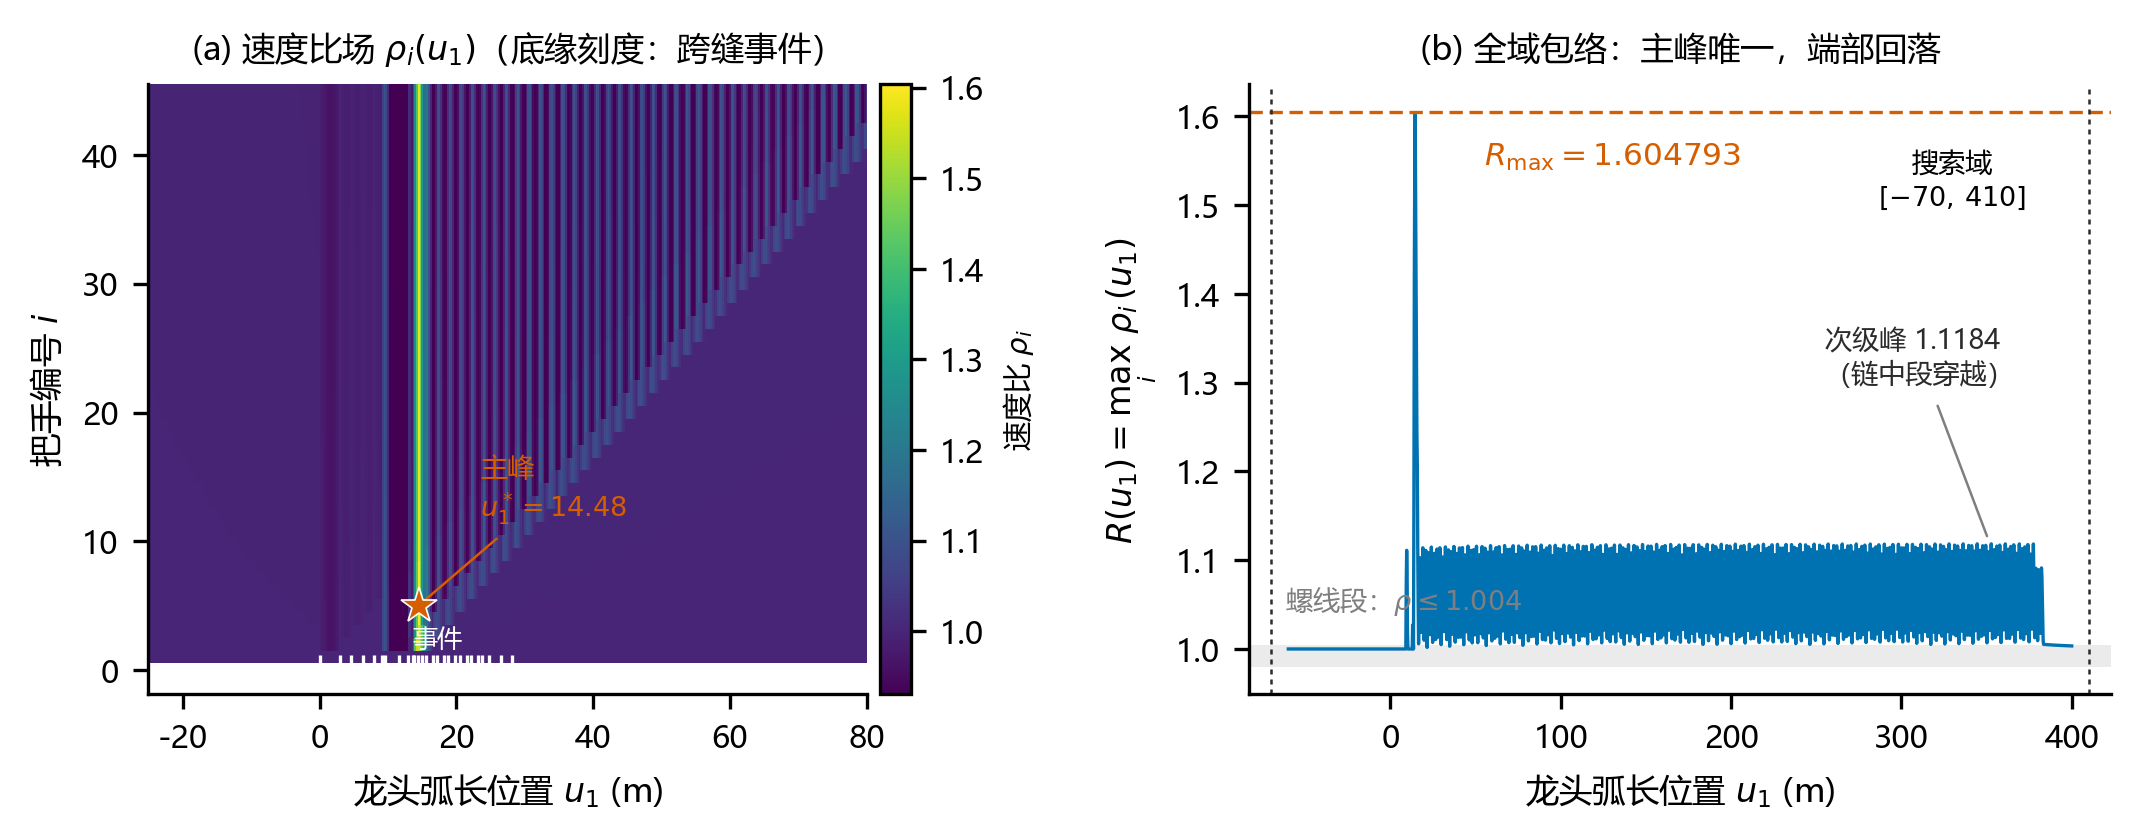
\includegraphics[width=0.65\textwidth]{figures/fig_问题五速度比场.png}
\caption{速度比场全景：（a）比场热力图 $\rho_i(u_1)$（底缘刻度为把手跨缝事件，星标为主峰）；（b）全域包络 $R(u_1)$——主峰唯一、次级峰 $1.1184$、端部回落至 $\le1.004$，搜索域截断 $[-70,410]$ 合理}
\label{fig:q5field}
\end{figure}

\begin{figure}[H]
\centering
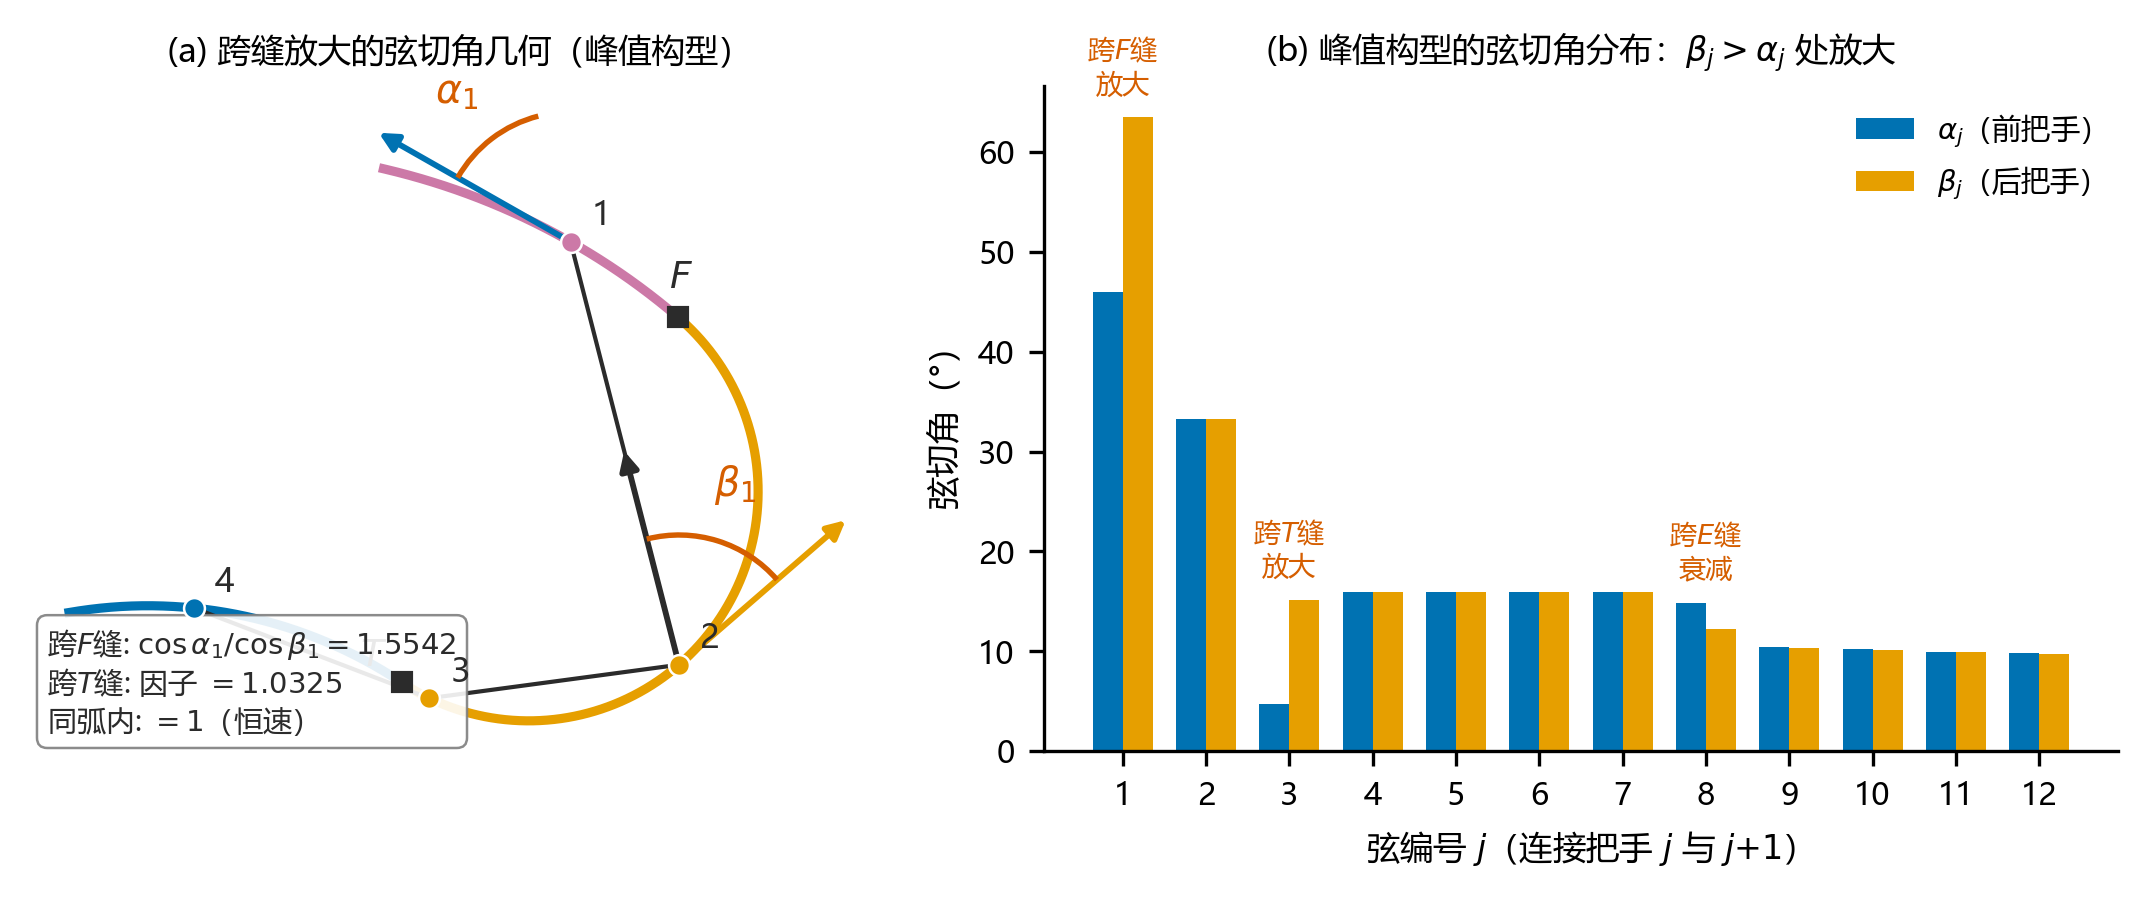
\includegraphics[width=0.61\textwidth]{figures/fig_问题五速度传递机理.png}
\caption{峰值机理：（a）跨缝放大的弦切角几何（峰值构型，弦在前端平、后端横）；（b）峰值构型的弦切角分布——$\beta_j>\alpha_j$ 的跨缝弦（$F$、$T$）产生放大，同弧内 $\alpha_j=\beta_j$ 比值恒 1}
\label{fig:q5mech}
\end{figure}

\subsubsection{扩展：调头曲线长度与行进速度的权衡}
对问题四弧–线–弧优化曲线（$R_1=0.8251$、$R_2=0.8978$ m、$L^{*}=10.0642$ m）重复模型 B 流程，得到比“权衡”更强的结论。其一，深弯弧的几何刚性：弧 2$'$ 弧长仅 $1.558\,\text{m}$ 小于相邻弦长 $1.65\,\text{m}$，相邻两把手不可能同时位于该弧上。其二，\textbf{速度比爆炸}：密扫显示 $\rho_{\max}^{\mathrm{alt}}$ 达 $8.6\sim22.7$（分支尖刺），且数学根源在于 $R_1\to D_{\text{body}}/2=0.825\,\text{m}$ 的\textbf{临界半径退化}——$R\to D/2^+$ 时弧上弦趋于直径、弦切角 $\psi\to90^\circ$、弦长方程的隐函数雅可比 $\partial\|C(u_2)-C(u_1)\|/\partial u_2\to0$，速度比 $|du_{i+1}/du_i|\sim(R-D/2)^{-1/2}\to\infty$，故 $v^{*}_{\mathrm{alt}}\to0$（数值上 $\le0.088\,\text{m/s}$，下降 $\ge93\%$，图~\ref{fig:q5trade}）。

\textbf{“盘得紧”与“跑得快”不可兼得}：问题四“能变短”的最优解位于可跟随性临界边界，静态几何可行（弦解存在、无碰撞），但运动学上全龙几乎不能行进。若表演同时要求高速与紧凑调头，应回到基线两弧，或在“调头曲线长度—龙头容许速度”的帕累托前沿上远离临界半径折中选点。该分析把全题的几何优化（问题三、四）与运动学约束（问题一、二、五）闭合为完整的设计框架。

\begin{figure}[H]
\centering
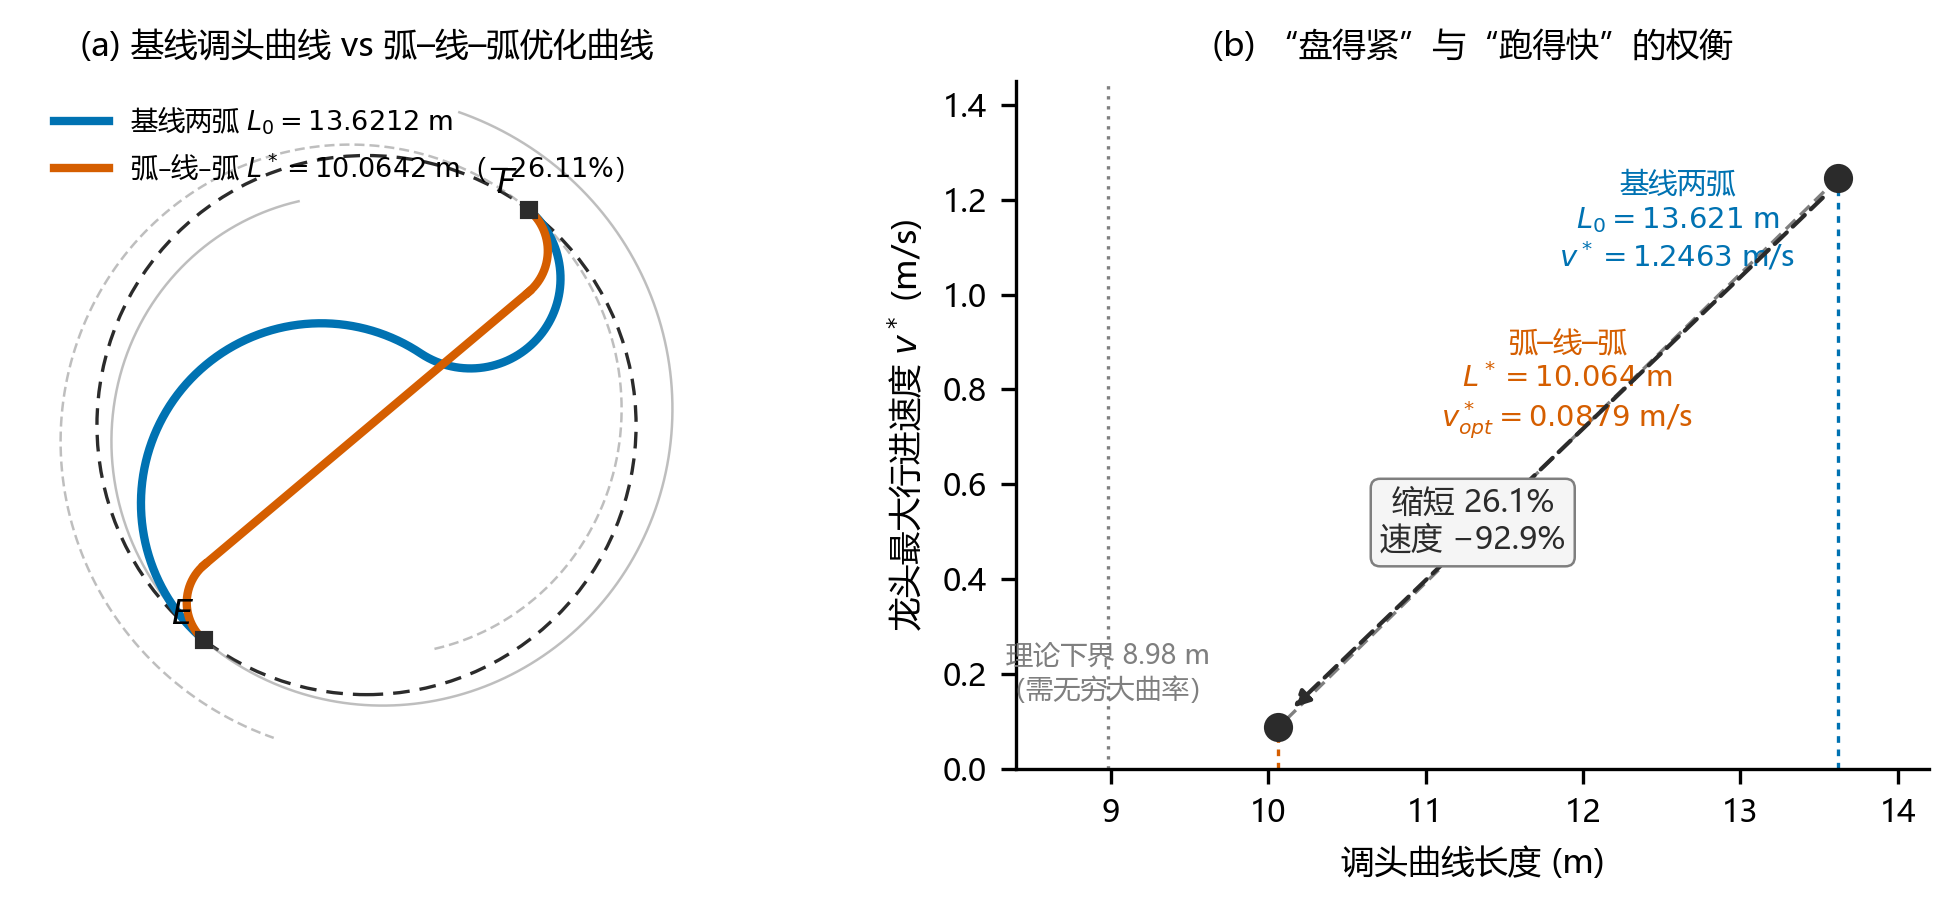
\includegraphics[width=0.74\textwidth]{figures/fig_问题五结构权衡.png}
\caption{结构权衡：（a）基线两弧曲线 vs 弧–线–弧优化曲线；（b）“调头曲线长度—龙头容许速度”权衡——缩短 $26.11\%$ 的代价是 $v^{*}$ 下降 $\ge93\%$（临界半径处趋于零）}
\label{fig:q5trade}
\end{figure}

\subsubsection{正确性验证与问题五小结}
运动学内核三重验证：弦长残差 $\le1.26\times10^{-13}\,\text{m}$；中心差分与弦切角递推偏差 $\le9.2\times10^{-9}\,\text{m/s}$；$u_1=14$ 处速度比与问题四已知值 $1.422195263$ 完全一致（偏差 $0$）。同一峰位由黄金分割、驻点求根与全域细密扫描（$\Delta=0.02$，得 $1.604793377$）三条途径互证（互差 $\le5\times10^{-15}$）。

\textbf{问题五小结}：由齐次性引理把“时间 $\times$ 把手”无穷族约束化为一元全局最大化，经事件分解、驻点求根与两层认证求得速度比场全局峰 $R_{\max}=1.604793379$（跨 $F$ 缝因子 $1.5542$ $\times$ 跨 $T$ 缝因子 $1.0325$，弧内恒速），最终
\begin{equation}
v^{*}=1.246266\ \text{m/s},\qquad
t^{*}_{5}=11.618680\ \text{s 时把手 4--8 并列达到 }2\,\text{m/s};
\end{equation}
并揭示调头曲线长度与行进速度的定量权衡：缩短调头曲线的代价由弦切角机制放大，临界半径（$R\to D/2$）处龙头容许速度趋于零。

%% ========================================================
%% 模型灵敏度与鲁棒性测试
%% ========================================================
\section{模型灵敏度与鲁棒性测试}\label{sec:sens}

以问题五的龙头最大容许速度 $v^{*}=2/R_{\max}$ 为检验对象（其答案对几何与运动学参数最敏感、工程意义最直接），做两级测试：参数\textbf{灵敏度}（确定性单参数扰动）与\textbf{鲁棒性}（随机速度波动的蒙特卡洛仿真）。

\textbf{（一）参数灵敏度}。(1) \textbf{龙身弦长 $D_{\text{body}}\pm5\%$}（板凳加工公差）：$v^{*}$ 仅变化 $+0.06\%\sim+0.20\%$，归一化灵敏度 $S_D=\Delta(v^{*}/v^{*}_0)\big/\Delta(D/D_0)\approx0.015$——模型对制造公差\textbf{稳健}。(2) \textbf{两弧半径比 $k=R_1/R_2$}（改变调头曲线几何，两弧族长度不变）：$k=1.5$（$R_2$ 增至 $1.80\,\text{m}$）时 $v^{*}=1.3773\,\text{m/s}$（$+10.5\%$）——弧半径增大使弦切角减小、跨缝放大减弱；$k=3$（$R_2$ 减至 $1.13\,\text{m}$）时粗扫出现 $4$ 处\textbf{弦解失效点}，即链条存在无法跟随的区间，该曲线不可行。故在保持全程可跟随的前提下，减小 $k$（增大 $R_2$）可提升容许速度，题目设定 $k=2$ 位于可行域内。(3) \textbf{数值参数}：弦解精度 $\mathrm{xtol}\in[10^{-14},10^{-10}]$ 与差分步长 $h\in[10^{-7},10^{-5}]$ 扰动下 $R_{\max}$ 偏差 $\le 2.4\times10^{-10}$，数值实现完全稳定。

\textbf{（二）鲁棒性蒙特卡洛}。设龙头实际速度含随机波动 $v_{\text{head}}(t)=\bar v\,(1+\varepsilon(t))$，$\varepsilon$ 为相关时间 $\tau=0.5\,\text{s}$ 的 Ornstein–Uhlenbeck 过程、标准差 $\sigma\in\{2\%,5\%\}$；对 $\bar v=v^{*}$ 与 $\bar v=0.95\,v^{*}$ 两档各仿真 $N=2000$ 次（每步由预计算的速度比场插值得到 $\max_i v_i$）。结果（图~\ref{fig:q5sens}）：以\textbf{满速 $v^{*}$ 行进时没有任何波动裕度}——$\sigma=2\%$ 的微小波动即带来 $59\%$ 的超限概率（$\sigma=5\%$ 时 $68\%$）；将运行速度降至 $0.95\,v^{*}\approx1.184\,\text{m/s}$ 后，$\sigma=2\%$ 波动下的超限概率降至 $0.9\%$。工程含义：$v^{*}$ 是理论临界值，实际编排应预留约 $5\%$ 的速度裕度（龙头按 $\approx1.18\,\text{m/s}$ 行进），方能在人力驱动的正常波动下保证各把手速度不超 $2\,\text{m/s}$。

\begin{figure}[H]
\centering
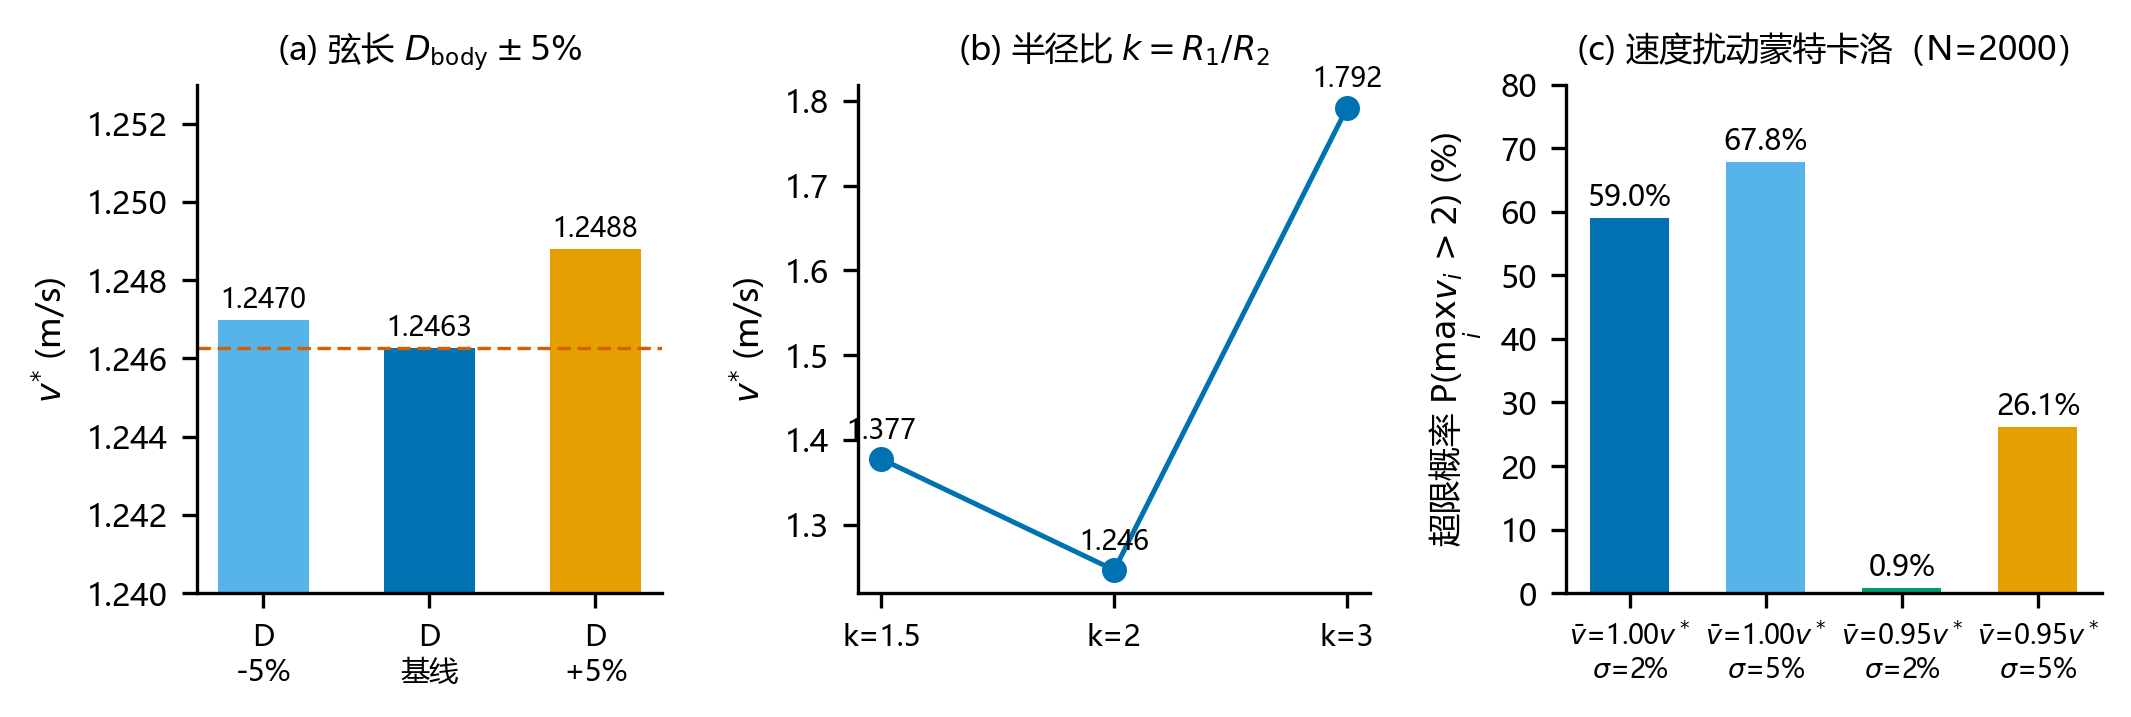
\includegraphics[width=0.88\textwidth]{figures/fig_问题五灵敏度鲁棒性.png}
\caption{灵敏度与鲁棒性测试：（a）龙身弦长 $\pm5\%$ 扰动下 $v^{*}$ 仅变化 $\le0.2\%$；（b）半径比 $k$ 扫描——$k=1.5$ 时 $v^{*}$ 提升 $10.5\%$，$k=3$ 出现弦解失效（不可跟随）；（c）OU 速度扰动的蒙特卡洛超限概率——满速无裕度，按 $0.95\,v^{*}$ 运行且 $\sigma=2\%$ 时超限概率 $<1\%$}
\label{fig:q5sens}
\end{figure}

%% ========================================================
%% 模型的评价与优缺点分析
%% ========================================================
\section{模型的评价与优缺点分析}

\textbf{总体评价}\quad 本文以“刚体铰接链在给定曲线上的逆运动学”为主线建立覆盖五问的统一体系：几何逆推与弦切角速度传递贯穿始终，从单一螺线推广到复合轨迹，再以齐次性约化把速度安全约束化为一元全局优化，形成“几何构造—运动学求解—干涉检测—参数与结构优化—安全认证”逐层递进的框架；各问结果均经独立方法交叉验证，关键结论附有解析解释（不变性定理、同弧段恒速引理、跨缝因子分解），保证结果既精确（$10^{-9}$ 量级）又可解释。

\textbf{优点}\quad (1) \textbf{框架统一}：逆推法与速度递推在各问间自然推广（螺线$\to$复合轨迹$\to$速度比场），问题三的入口曲率为问题四的相切衔接奠基、问题四的速度场直接给出问题五的提速瓶颈，全题闭环。(2) \textbf{解析与数值深度结合}：S 形调头曲线几何全闭式、两弧族长度不变性定理、同弧段恒速引理与跨缝因子分解，使数值结果均有解析骨架支撑，避免“黑盒输出”。(3) \textbf{数值可靠性措施完备}：弦长残差 $10^{-13}\,\text{m}$、差分与递推互验、SAT 与 shapely 双判据、CCD 消除隧道效应；问题五以事件子段穷举加 Lipschitz 剪枝证书给出宽度 $<10^{-9}$ 的严格认证。(4) \textbf{全局最优性有结构保证}：问题三的单调性二分、问题四的不变性定理、问题五的事件分解，均从结构上排除无效搜索与漏峰可能。

\textbf{缺点与改进方向}\quad (1) \textbf{理想化假设}：忽略把手间隙、板凳形变与人力驱动的速度波动——波动的幅值影响已由第\ref{sec:sens}节蒙特卡洛检验，但未建模扰动的频谱结构。(2) \textbf{碰撞检测复杂度}：$O(N^{2})$ 对检测 $\times$ 密集时间扫描，可用层次包围盒预筛或对螺线局部曲率展开将间隙解析化。(3) \textbf{认证的经验成分}：问题三的可行性单调性、问题五的 Lipschitz 常数与搜索域截断依赖数值论证，可引入区间算术或自动微分严格化。(4) \textbf{目标单一与效率}：问题四仅以长度为目标（问题五已证其最优解位于临界半径、容许速度趋于零），应建立“长度—速度”双目标规划；主流程纯 Python 约 $30$ 分钟，可向量化加速。

\textbf{模型的推广}\quad 本文框架可直接用于铰接列车弯道限速、缆索牵引系统张力校核、AGV 铰接编队路径认证等“链式刚体沿轨道运动”类问题（把 $2\,\text{m/s}$ 换成相应安全阈值，$v^{*}=2/R_{\max}$ 的约化同样成立）；“事件分解 + Lipschitz 认证”亦可作为一维全局优化的通用认证范式。

\begin{thebibliography}{9}
\bibitem{tanaka} Tanaka K, Hori S, Wang H O. Multi-objective control of a vehicle with triple trailers[C]//Proceedings of the 40th IEEE Conference on Decision and Control. Orlando, FL: IEEE, 2001.
\bibitem{lekkas} Lekkas A M, Dahl A R, Breivik M, Fossen T I. Continuous-curvature path generation using Fermat's spiral[J]. Modeling, Identification and Control, 2013, 34(4): 183--198.
\bibitem{verscheure} Verscheure D, Demeulenaere B, Swevers J, De Schutter J, Diehl M. Time-optimal path tracking for robots: a convex optimization approach[J]. IEEE Transactions on Automatic Control, 2009, 54(10): 2318--2327.
\bibitem{artunedo} Artuñedo A, Villagra J, Godoy J. Jerk-limited time-optimal speed planning for arbitrary paths[J]. Journal of Intelligent \& Robotic Systems, 2021, 103: 21.
\end{thebibliography}

% ============================================================
% 附录：核心源代码
% ============================================================
\newpage
\begin{appendices}

\section{动态推演与位置可视化程序}
\begin{lstlisting}
import numpy as np
import os
import matplotlib.pyplot as plt

PITCH = 0.55
B = PITCH / (2 * np.pi)
THETA0 = 32 * np.pi
HEAD_L, BODY_L = 3.41, 2.20
HOLE_OFF = 0.275
D_HEAD = HEAD_L - 2 * HOLE_OFF
D_BODY = BODY_L - 2 * HOLE_OFF

def pos(theta):
    r = B * theta
    return np.array([r * np.cos(theta), r * np.sin(theta)])

def arc_len(theta):
    return 0.5 * B * (theta * np.sqrt(theta * theta + 1) + np.arcsinh(theta))

F0 = arc_len(THETA0)

def theta_head(t):
    lo, hi = 0.0, THETA0
    for _ in range(80):
        mid = 0.5 * (lo + hi)
        if F0 - arc_len(mid) > t:
            lo = mid
        else:
            hi = mid
    return 0.5 * (lo + hi)

def next_theta(th, d):
    P = pos(th)
    hi = 0.8
    while np.linalg.norm(pos(th + hi) - P) < d and hi < 3.2:
        hi *= 2.0
    lo = 0.0
    for _ in range(80):
        mid = 0.5 * (lo + hi)
        if np.linalg.norm(pos(th + mid) - P) > d:
            hi = mid
        else:
            lo = mid
    return th + 0.5 * (lo + hi)

def all_thetas(t):
    ths = np.empty(224)
    ths[0] = theta_head(t)
    for i in range(223):
        ths[i + 1] = next_theta(ths[i], D_HEAD if i == 0 else D_BODY)
    return ths
\end{lstlisting}

\section{基于二阶中心差分与 Brent 求根的求解模块}
\begin{lstlisting}
from scipy.optimize import brentq

DT = 0.1  # 离散化时间步长

def _dist_u(u, th, d):
    P = pos(th)
    return np.linalg.norm(pos(th + u) - P) - d

def next_theta_precise(th, d):
    hi = 0.8
    while _dist_u(hi, th, d) < 0 and hi < 3.2:
        hi *= 2.0
    u_root = brentq(lambda u: _dist_u(u, th, d), 0.0, hi, xtol=1e-12)
    return th + u_root

def compute_velocities_central_diff(pos_small):
    # 基于二阶精度中心差分法的速度场计算
    vel_small = np.empty_like(pos_small[:, :, 0])
    vel_small[0] = np.linalg.norm(pos_small[1] - pos_small[0], axis=1) / DT
    vel_small[-1] = np.linalg.norm(pos_small[-1] - pos_small[-2], axis=1) / DT
    vel_small[1:-1] = np.linalg.norm(pos_small[2:] - pos_small[:-2], axis=2) / (2 * DT)
    return vel_small
\end{lstlisting}

\section{包含连续碰撞检测 (CCD) 与 SAT 的干涉边界搜索程序}
\begin{lstlisting}
WIDTH = 0.30

def bench_rect(i, Ps):
    p0, p1 = Ps[i], Ps[i + 1]
    L = HEAD_L if i == 0 else BODY_L
    v = p1 - p0
    u = v / np.linalg.norm(v)
    c = 0.5 * (p0 + p1)
    return c, u, L / 2.0, WIDTH / 2.0

def _project_interval(c, u, hlen, hwid, axis):
    n = np.array([-u[1], u[0]])
    radius = hlen * abs(np.dot(u, axis)) + hwid * abs(np.dot(n, axis))
    proj = np.dot(c, axis)
    return proj - radius, proj + radius

def _point_in_rect(p, r, tol=1e-9):
    c, u, hlen, hwid = r
    n = np.array([-u[1], u[0]])
    du = np.dot(p - c, u)
    dn = np.dot(p - c, n)
    return abs(du) <= hlen + tol and abs(dn) <= hwid + tol

def rect_corners(r):
    c, u, hlen, hwid = r
    n = np.array([-u[1], u[0]])
    return np.array([
        c + hlen * u + hwid * n,
        c + hlen * u - hwid * n,
        c - hlen * u + hwid * n,
        c - hlen * u - hwid * n,
    ])

def rects_collide(r1, r2, tol=1e-4):
    for p in rect_corners(r1):
        if _point_in_rect(p, r2, tol):
            return True
    for p in rect_corners(r2):
        if _point_in_rect(p, r1, tol):
            return True
    axes = [r1[1], np.array([-r1[1][1], r1[1][0]]),
            r2[1], np.array([-r2[1][1], r2[1][0]])]
    for ax in axes:
        lo1, hi1 = _project_interval(r1[0], r1[1], r1[2], r1[3], ax)
        lo2, hi2 = _project_interval(r2[0], r2[1], r2[2], r2[3], ax)
        if hi1 - lo2 < tol or hi2 - lo1 < tol:
            return False         
    return True

def detect_collision(ths, first_only=True):
    Ps = np.array([pos(th) for th in ths])
    n = len(ths) - 1 
    rects = [bench_rect(i, Ps) for i in range(n)]
    hits = []
    for i in range(n):
        for j in range(i + 1, n):
            if j - i == 1: 
                continue
            if rects_collide(rects[i], rects[j]):
                hits.append((i + 1, j + 1)) 
                if first_only:
                    return True, hits
    return bool(hits), hits

def find_stop_time(t_lo=0.0, t_hi=1000.0, tol=1e-3):
    def has_coll(t):
        ths = all_thetas(t)
        c, _ = detect_collision(ths)
        return c

    step = 20.0
    t = 0.0
    while not has_coll(t):
        t += step
        if t > t_hi:
            raise RuntimeError("Out of bounds")
    t_hi = t
    t_lo = max(0.0, t - step)

    while t_hi - t_lo > tol:
        t_mid = 0.5 * (t_lo + t_hi)
        if has_coll(t_mid):
            t_hi = t_mid
        else:
            t_lo = t_mid
    return t_hi
\end{lstlisting}
\section{问题三：最小螺距二分搜索程序}
\begin{lstlisting}
# 可行性判定：螺距 p 下沿螺线盘入至调头空间边界, 复用问题二 SAT 判据
def feasible(p, coarse_step=8):
    b = p / (2 * np.pi)
    th_end = 9 * np.pi / p                 # 边界条件 r(theta_end) = 4.5
    ths = [32 * np.pi]                     # 第 16 圈 A 点出发
    while ths[-1] > th_end:                # 逐把手逆推(同问题一)
        d = D_HEAD if len(ths) == 1 else D_BODY
        th = ths[-1]
        f = lambda u: np.linalg.norm(pos(th + u) - pos(th)) - d
        ths.append(th + brentq(f, 0.4 * d, 2.6 * d))
        if len(ths) % coarse_step == 0 and detect_collision(ths)[0]:
            return False                   # 宽相短路: 中途相撞即不可行
    return not detect_collision(ths)[0]

# 可行性关于螺距单调(螺距增大则相邻圈间隙增大) -> 二分搜索
lo, hi = 0.40, 0.55
while hi - lo > 1e-4:
    mid = 0.5 * (lo + hi)
    if feasible(mid):
        hi = mid                           # 可行 -> 试更小螺距
    else:
        lo = mid                           # 不可行 -> 抬高下界
print(f"最小螺距 p* = {hi:.4f} m")          # 输出 p* ≈ 0.4503 m
\end{lstlisting}

\section{问题四：S 形调头曲线解析几何与复合轨迹逆推程序}
\begin{lstlisting}
def s_curve_geom(p=1.7, R_space=4.5):
    """闭式解出 S 形曲线: 切点/圆心/半径/扫角 (R1 = 2*R2)."""
    b = p / (2 * np.pi)
    thA = R_space / b                      # 入口极角 = 9*pi/p
    E = np.array([b*thA*np.cos(thA), b*thA*np.sin(thA)])
    dv = np.array([np.cos(thA)-thA*np.sin(thA), np.sin(thA)+thA*np.cos(thA)])
    tE = -dv / np.linalg.norm(dv)          # 盘入行进方向
    nE = np.array([-tE[1], tE[0]])         # 左法线
    F, tF = -E, tE                         # 中心对称: 出口切点与方向
    dlt = F - E
    S = -np.dot(dlt, dlt) / (2 * np.dot(dlt, nE))   # 外切条件定 R1+R2
    R1, R2 = 2*S/3, S/3
    O1, O2 = E - R1*nE, F + R2*nE
    m = (O2 - O1) / np.linalg.norm(O2 - O1)
    gam = np.arctan2(*( (E-O1)[::-1] )) - np.arctan2(*m[::-1])
    gam %= 2 * np.pi                       # 两弧扫角(相等)
    L1, L0 = R1*gam, (R1+R2)*gam
    return dict(E=E, F=F, O1=O1, O2=O2, R1=R1, R2=R2, gam=gam, L1=L1, L0=L0)

def curve_point(u, g, sA):
    """复合轨迹 C: 盘入螺线 | 弧1 | 弧2 | 盘出螺线 (弧长参数 u)."""
    if u < 0:   return spiral_point(sA - u)
    if u <= g['L1']:
        phi = np.arctan2(*(g['E']-g['O1'])[::-1]) - u / g['R1']
        return g['O1'] + g['R1']*np.array([np.cos(phi), np.sin(phi)])
    if u <= g['L0']:
        phi = np.arctan2(*(g['T']-g['O2'])[::-1]) + (u-g['L1']) / g['R2']
        return g['O2'] + g['R2']*np.array([np.cos(phi), np.sin(phi)])
    return -spiral_point(sA + (u - g['L0']))

def config_at(t, g, sA):
    """逆推法推广: 弦长方程逐节求把手弧长位置, 再由切向递推速度."""
    us = np.empty(224); us[0] = t
    for i in range(223):
        di = D_HEAD if i == 0 else D_BODY
        P = curve_point(us[i], g, sA)
        f = lambda dl: np.linalg.norm(curve_point(us[i]-dl, g, sA) - P) - di
        us[i+1] = us[i] - brentq(f, 0.4*di, 2.6*di, xtol=1e-12)
    return us
\end{lstlisting}

\section{问题五：速度比场全局优化与认证程序}
\begin{lstlisting}
# 齐次性约化: v* = 2/R_max, R_max = max rho_i(u1) (v=1 虚拟行进的速度比场)
def config_at(u1):                     # 复合轨迹上的弦长逆推 (同问题4)
    us = np.empty(224); us[0] = u1
    for i in range(223):
        d = D_ALL[i]; P = curve_point(us[i])
        f = lambda dl: np.linalg.norm(curve_point(us[i]-dl) - P) - d
        us[i+1] = us[i] - brentq(f, 0.4*d, 2.6*d, xtol=1e-12)
    return us

def velocities(us):                    # 弦切角速度传递 rho_{i+1} = rho_i * cos(a)/cos(b)
    Ps = positions(us); v = np.empty(224); v[0] = 1.0
    for i in range(223):
        e = Ps[i+1] - Ps[i]; e /= np.linalg.norm(e)
        v[i+1] = v[i] * np.dot(curve_tangent(us[i]), e) \
                      / np.dot(curve_tangent(us[i+1]), e)
    return v

def rho_max(u1): return float(np.max(velocities(config_at(u1))))

# ---- 对照: 均匀网格采样 (恒低估峰值, 验证结构化搜索的必要性) ----
R_hat = max(rho_max(u1) for u1 in np.arange(U_LO, U_HI + 1e-9, step))
v_star_A = 2.0 / R_hat

# ---- 主方法: 接缝事件分解 + 光滑段精确最大化 ----
def golden_max(lo, hi):                # bounded Brent, 仅依赖单峰性
    r = minimize_scalar(lambda u: -rho_max(u), bounds=(lo, hi),
                        method="bounded", options={"xatol": 1e-11})
    return float(r.x)
# 粗扫剪枝: R>1.25 的连通域 [13.0,16.25] 进入精搜
R_max_B = rho_max(golden_max(13.0, 16.25))

# ---- 严格认证: 驻点求根 + Lipschitz 剪枝证书 + 事件子段穷举 ----
def dR(u, h=1e-6): return (rho_max(u+h) - rho_max(u-h)) / (2*h)
xs = np.linspace(14.0, 15.0, 121)                    # 符号扫描隔离根
sgn = [k for k in range(120) if dR(xs[k])*dR(xs[k+1]) < 0]
u_star = brentq(dR, xs[sgn[0]], xs[sgn[0]+1], xtol=1e-12)
R_star = rho_max(u_star); v_star = 2.0 / R_star
# 峰窗按事件切子段逐段黄金分割 (认证) + 域外 Lipschitz 剪枝证书
# R <= 粗扫最大值 + L*Delta/2 (L=数值导数上界 x1.3), 验证 << R_star
\end{lstlisting}
\end{appendices}
\end{document}

